\documentclass[cn,11pt, simple]{elegantbook}

\title{TikZ学习入门之葵花宝典}
\subtitle{未完续}

\author{八一}
\institute{ hoganbin1995@outlook.com}
\weixin{八一考研数学竞赛}
\date{ \today}

\usepackage{amsmath}
\usepackage{url}
\usepackage{xcolor}
\usepackage{color}
\usepackage{cancel}
\usepackage{pgfornament}
\usepackage{calligra}
\usepackage{pstricks-add}
%\usepackage{tkz-linknodes}
\usepackage{metalogo}
\usepackage{scalerel} %\scaleobj{1.5}{} 缩放公式大小
\usepackage{siunitx} %需用到\ang[options]{degrees}命令
\definecolor{pink}{RGB}{249,164,186}
\definecolor{grassgreen}{RGB}{128,255,0}
\def\sgn{\mathop{\rm sgn}}
%\setCJKmainfont[AutoFakeBold,AutoFakeSlant]{STSong}
%\setCJKsansfont[AutoFakeBold,AutoFakeSlant]{KaiTi}
%\setCJKmonofont[AutoFakeBold,AutoFakeSlant]{STFangsong}
%\usepackage{verbatim}
%\usepackage[active,tightpage]{preview}
%\PreviewEnvironment{tikzpicture}
%\setlength\PreviewBorder{5pt}
\usepackage{tikz,pgfplots}
\usepackage{circuitikz}
\usetikzlibrary{
	shapes.geometric,   %几何形状
	calc,               %计算
	positioning,       %用于提供位置表达语句的支持,通俗讲就是定位
	arrows.meta,        %提供各种箭头
	automata,          %绘制状态转换图
	matrix,            %构建矩阵
	topaths,%用于to/edge算子构建的路径
	shapes.misc,       %约分
	chains,          %绘制链状图形的库,一般画流程图必需的库
	shadings,          %提供已定义好的图案如菱形
	quotes,    %提供引用句法
	angles,   %用来标示角
	patterns,  %定义图样,如条纹
	fadings,   %用于灰度图
	fit,   %创建数个坐标点
	decorations.pathmorphing,   %装饰线
	decorations.text,
	quotes,through,
	intersections, %两个路径的交点
	backgrounds,   %背景路径
	shapes,
	arrows,    %箭头路径
	snakes,
	mindmap, %思维导图
	shadows,
	circuits.ee.IEC%电路图
}
\tikzstyle{state}=[circle,label=below:$r$,
thick,
minimum size=1.2cm,
draw=blue!80,
fill=blue!20]
\tikzstyle{state2}=[circle,label=below:$e$,
thick,
minimum size=1.2cm,
draw=blue!80,
fill=blue!20]
\tikzstyle{state3}=[circle,label=below:$a$,
thick,
minimum size=1.2cm,
draw=blue!80,
fill=blue!20]
\tikzstyle{state4}=[circle,label=below:$d$,
thick,
minimum size=1.2cm,
draw=blue!80,
fill=blue!20]
% The measurement vector is represented by an orange circle.
\tikzstyle{measurement}=[circle,
thick,
minimum size=1.2cm,
draw=orange!80,
fill=orange!25]

% The control input vector is represented by a purple circle.
\tikzstyle{input}=[circle,
thick,
minimum size=1.2cm,
draw=purple!80,
fill=purple!20]

% The input, state transition, and measurement matrices
% are represented by gray squares.
% They have a smaller minimal size for aesthetic reasons.
\tikzstyle{matrx}=[rectangle,
thick,
minimum size=1cm,
draw=gray!80,
fill=gray!20]

% The system and measurement noise are represented by yellow
% circles with a "noisy" uneven circumference.
% This requires the TikZ library "decorations.pathmorphing".
\tikzstyle{noise}=[circle,
thick,
minimum size=1.2cm,
draw=yellow!85!black,
fill=yellow!40,
decorate,
decoration={random steps,
	segment length=2pt,
	amplitude=2pt}]

% Everything is drawn on underlying gray rectangles with
% rounded corners.
\tikzstyle{background}=[rectangle,
fill=gray!10,
inner sep=0.2cm,
rounded corners=5mm]





\usepackage{scalerel} %\scaleobj{1.5}{} 缩放公式大小
\newcommand\hcancel[2][black]{\setbox0=\hbox{#2}\rlap{\raisebox{.45\ht0}{\textcolor{#1}{\rule{\wd0}{1pt}}}}#2}


\definecolor{pink}{RGB}{249,164,186}
\definecolor{grassgreen}{RGB}{128,255,0}

\pgfkeys{/pgf/decoration/.cd,
	stipple density/.store in=\pgfstippledensity,
	stipple density=.1,
	stipple scaling function/.store in=\pgfstipplescalingfunction,
	stipple scaling function=sin(\pgfstipplex*180)*0.875+0.125,
	stipple radius/.store in=\pgfstippleradius,
	stipple radius=0.25pt
}
\pgfdeclaredecoration{stipple}{draw}{
	\state{draw}[width=\pgfdecorationsegmentlength]{
		\pgfmathparse{\pgfdecoratedcompleteddistance/\pgfdecoratedpathlength}%
		\let\pgfstipplex=\pgfmathresult%
		\pgfmathparse{int(\pgfstippledensity*100)}%
		\let\pgfstipplen=\pgfmathresult
		\pgfmathloop
		\ifnum\pgfmathcounter<\pgfmathresult\relax
		\pgfpathcircle{%
			\pgfpoint{(rnd)*\pgfdecorationsegmentlength}%
			{(\pgfstipplescalingfunction)*(rnd^4)*\pgfdecorationsegmentamplitude+\pgfstippleradius}}% 
		{\pgfstippleradius}%
		\repeatpgfmathloop
	}
}

\tikzset{stipple/.style={
		decoration={stipple, segment length=2pt, #1},
		decorate,
		fill
}}
% end of stippling code

\newcommand\DrawBlock[3]{
	\ifx#1b\relax
	\path[draw]
	(lm\the\numexpr#2-1\relax) -- ++(0,0,#3) coordinate (blocklf)
	(bm\the\numexpr#2-1\relax) -- ++(0,0,#3) coordinate (blocklb)
	(lm#2) -- ++(0,0,#3) coordinate (blockrf)
	(bm#2) -- ++(0,0,#3) coordinate (blockrb);
	\filldraw[fill=white,draw=black]
	(lm\the\numexpr#2-1\relax) -- (blocklf) -- (blocklb) -- (blockrb) -- (blockrf) -- (lm#2);
	\else  
	\ifx#1f\relax
	\path[draw]
	(fm\the\numexpr#2-1\relax) -- ++(0,0,#3) coordinate (blocklf)
	(lm\the\numexpr#2-1\relax) -- ++(0,0,#3) coordinate (blocklb)
	(fm#2) -- ++(0,0,#3) coordinate (blockrf)
	(lm#2) -- ++(0,0,#3) coordinate (blockrb);
	\filldraw[fill=white,draw=black]
	(fm\the\numexpr#2-1\relax) -- (blocklf) -- (blocklb) -- (blockrb) -- (blockrf) -- (fm#2);
	\fi
	\fi
	\draw (blocklf) -- (blockrf);
}

\tikzset{
	every picture/.style={
		>=latex,
		node distance=5mm and 5mm
		%有无and的区别见手册positioning部分
}}

%定义框形状
\tikzstyle{SS}      %开始结束
=[rounded corners, draw,rectangle]
\tikzstyle{IO}      %输入输出
=[trapezium, trapezium left angle=70, trapezium right angle=110, draw]
\tikzstyle{NR}      %内容
=[draw]
\tikzstyle{PD}      %判断
=[diamond, aspect=4, draw, inner sep=1.5pt]



%\usepackage{background}
%\definecolor{bg}{RGB}{58,95,205}
%\backgroundsetup{opacity=0.05,scale=1.2,angle=0,contents={
%		\begin{tikzpicture}
%		\node[minimum width=18cm,minimum height=25cm,inner sep=0pt,outer sep=0pt,](box){};
%		\fill[left color=bg!70!black!70,right color=bg!70!black] (box.south west)--(box.south east)--(box.north east)--(box.north west)--cycle;
%		\shade[inner color=bg!70!black,outer color=white!30!bg] (3,6)circle(.3cm);
%		\draw[opacity=.2,blue] (4,-6)circle(3cm);
%		\draw[opacity=.2,blue] (3,-5)circle(5cm);
%		\draw[opacity=.2,blue] (2,-3)circle(6cm);
%		\shade[inner color=bg!70!black,outer color=white!30!bg,xshift=-2cm,yshift=-11cm] (3,6)circle(.3cm);
%		\shade[inner color=bg!70!black,outer color=white!30!bg,xshift=1.3cm,yshift=-12cm] (3,6)circle(.3cm);
%		\shade[inner color=bg!70!black,outer color=white!30!bg,xshift=-4cm,yshift=-8cm] (3,6)circle(.3cm);
%		\shade[inner color=bg!70!black,outer color=white!30!bg,xshift=-6cm,yshift=-10cm] (3,6)circle(.3cm);
%		\shade[inner color=bg!70!black,outer color=white!30!bg,xshift=-6cm,yshift=-13cm] (3,6)circle(.3cm);
%		\end{tikzpicture}
%}}

%\usepackage{draftwatermark}
%\SetWatermarkText{\shortstack
%	{微信公众号:八一考研数学竞赛
%}}
%\SetWatermarkLightness{0.50}%设置水印亮度
%\SetWatermarkScale{0.3}%设置水印大小
\version{3.09}


\extrainfo{人生的意义,在于折腾}

\logo{logo.png}
\cover{cover.pdf}
\includeonly{class/ch01}



\begin{document}
\maketitle
\tableofcontents
% \thispagestyle{empty}
\mainmatter
\hypersetup{pageanchor=true}

\chapter*{前言}

在学习\LaTeX 与 TikZ过程中,八一发现到大家其学习\LaTeX 曲线陡峭,它并非所见即所得,可能一个微小的改动需要长时间的全文编译,而且代码并不能真正显示事物本来的样子,TikZ 的底层是 PGF(portable graphics format) ,即它是PGF 的前端。

它也并不是唯一可以在 \LaTeX 中画出漂亮图的宏包,比如 xfig 就可以代替它。另外 pstricks 和 metapost 都可以完成 TikZ 的工作;在PGF 中有很多优秀的并且可以独立于 PGF 之外运行的包。比如pgfpages宏包,它功能强大,可以合并多页,可以制作水印,可以将多页缩放到一个页面里;pgfplots宏包可直接调用一个axis环境和进行一些简单的优化来绘制函数并通过数据点拟合函数和散点图等。

那我们开始学习TikZ,首先得有个前提工作:这里的\lstinline|tikz|宏包的加载是必须的,而\lstinline|tikz|有两种使用方法:一种命令式用\lstinline|\tikz|命令,是行内模式;一种环境式用\lstinline|tikzpicture|环境命令包围起来,是行间模式。如下所示:
\begin{lstlisting}
\tikz{\draw (1,0) -- (0,1) -- (-1,0) -- (0,-1) -- cycle;} 
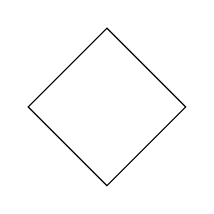
\begin{tikzpicture} 
\draw (1,0) -- (0,1) -- (-1,0) -- (0,-1) -- cycle; 
\end{tikzpicture}
\end{lstlisting}

行内模式对于注重内容的用户相对较少,基本不用,这种模式下直接调用而\lstinline|\tikz|命令。但不管是注重华丽表现效果还是注重内容的用户,总是会有需求需要某一整张图片来表达某些内容,而\lstinline|tikz|以及其他基于\lstinline|tikz|的宏包在命令行绘图这个领域是不错的。下面将主要使用\lstinline|tikzpicture|环境命令模式。

用\lstinline|tikz|绘制某个单独的图片而不是一般的A4页面推荐使用 standalone 类。如下所示:
\begin{lstlisting}
\documentclass[tikz,border=2pt]{standalone} 
\begin{document} 
\begin{tikzpicture} 
\draw[step=1,color=gray!40] (-2,-2) grid (2,2); 
\draw[->] (-3,0) -- (3,0); 
\draw[->] (0,-3) -- (0,3); 
\draw (0,0) circle (1);  
\end{tikzpicture} 
\end{document}
\end{lstlisting}

\chapter{基础准备}
\begin{introduction}
	\item 点
	\item 圆
	\item 矩形
	\item 抛物线
	\item 文本
	\item 直线
	\item 抛物线
	\item pgfplots
\end{introduction}
\section{点(Point Path)}
一行的中间高度画一个半径为一半行高的红点\tikz \filldraw [red ] (0.5 ex ,0.5ex ) circle [radius =0.5 ex ];使用coordinate命令或者path命令附带coordinate来定义一个点。
\begin{lstlisting}
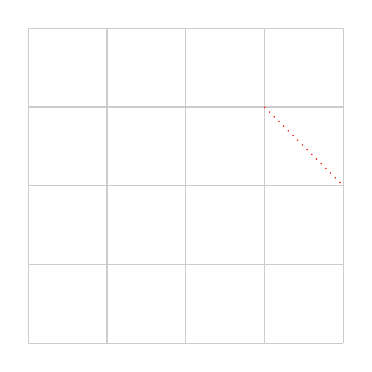
\begin{tikzpicture}
\draw[step=1,color=gray!40] (-2,-2) grid (2,2);
\path (1,1) coordinate (p1);
\coordinate (p2) at ( 2, 0);
\draw[dotted, red] (p1) -- (p2)  ;
\end{tikzpicture}
\end{lstlisting}
\begin{center}
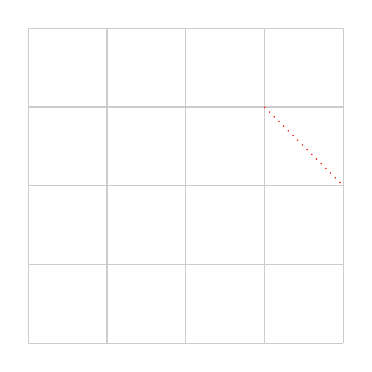
\begin{tikzpicture}
\draw[step=1,color=gray!40] (-2,-2) grid (2,2);
\path (1,1) coordinate (p1);
\coordinate (p2) at ( 2, 0);
\draw[dotted, red] (p1) -- (p2)  ;
\end{tikzpicture}
\end{center}
\subsection{控制点}
起点$x$的控制点 $y$,指的是曲线所在点 $x$ 处的切线方向指向 $y$ 点。如图所示。点 $x_{1} (0,0)$ 处的切线方向指向点$ y_{1} (1,1)$,点 $x_{2} (2,0)$ 点的切线方向指向点 $y_{2} (2,1)$,用法如下:
\begin{verbatim}
\draw[options] (x1,y1) .. controls (x2,y2) and (x3,y3) .. (x4,y4);
\end{verbatim}
\begin{lstlisting}
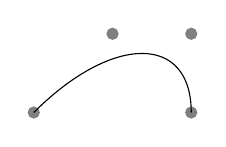
\begin{tikzpicture}
\filldraw[gray] (0,0) circle (2pt) (1,1) circle (2pt)
(2,1) circle (2pt) (2,0) circle (2pt);
\draw (0,0) .. controls (1,1) and (2,1) .. (2,0);
\end{tikzpicture}
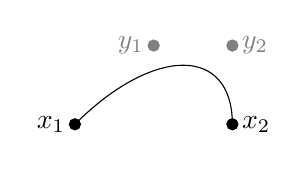
\begin{tikzpicture}
\filldraw (0,0) circle [radius =2 pt ] node [left ] {$ x _1$};
\filldraw [gray ] (1,1) circle [radius =2 pt ] node [left ] {$ y _1$};
\filldraw [gray ] (2,1) circle [radius =2 pt ] node [right ] {$ y_2$};
\filldraw (2,0) circle [radius =2 pt ] node [right ] {$ x _2$};
\draw (0,0) .. controls (1,1) and (2,1) .. (2,0); % 核心代码
\end{tikzpicture}
\begin{tikzpicture}
\draw (0,0) .. controls (1,1) and (2,1) .. (4,0);
\fill (1,1) circle (1pt) (2,1) circle (1pt);
\end{tikzpicture}
\end{lstlisting}
\begin{center}
	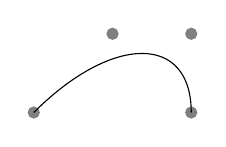
\begin{tikzpicture}
	\filldraw[gray] (0,0) circle (2pt) (1,1) circle (2pt)
	(2,1) circle (2pt) (2,0) circle (2pt);
	\draw (0,0) .. controls (1,1) and (2,1) .. (2,0);
	\end{tikzpicture}
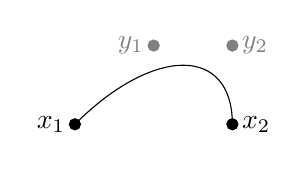
\begin{tikzpicture}
\filldraw (0,0) circle [radius =2 pt ] node [left ] {$ x _1$};
\filldraw [gray ] (1,1) circle [radius =2 pt ] node [left ] {$ y _1$};
\filldraw [gray ] (2,1) circle [radius =2 pt ] node [right ] {$ y_2$};
\filldraw (2,0) circle [radius =2 pt ] node [right ] {$ x _2$};
\draw (0,0) .. controls (1,1) and (2,1) .. (2,0); % 核心代码
\end{tikzpicture}
\begin{tikzpicture}
\draw (0,0) .. controls (1,1) and (2,1) .. (4,0);
\fill (1,1) circle (1pt) (2,1) circle (1pt);
\end{tikzpicture}
\end{center}
再来一个控制点的例子:用控制点画一个半圆,见下图。当然,本例只是阐释控制点,实际中很少用这种方式画半圆。
\begin{lstlisting}
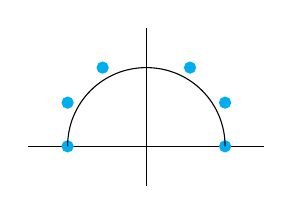
\begin{tikzpicture}
\draw (- 1.5,0) -- (1.5,0);
\draw (0,- 0.5) -- (0,1.5);
% show the control points
\filldraw [gray ] ( - 1,0) circle [radius =2 pt ]
(1,0) circle [radius =2 pt ]
[cyan ] (- 1,0.555) circle [radius =2 pt ]
[cyan ] (- 0.555,1) circle [radius =2 pt ]
[cyan ] (0.555,1) circle [radius =2 pt ]
[cyan ] (1,0.555) circle [radius =2 pt ];
\draw (- 1,0) .. controls (- 1,0.555) and (- 0.555,1) .. (0,1) .. controls (0.555,1) and (1,0.555) .. (1,0);
\end{tikzpicture}
\end{lstlisting}
\begin{center}
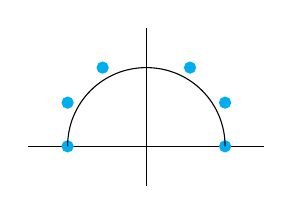
\begin{tikzpicture}
\draw (- 1.5,0) -- (1.5,0);
\draw (0,- 0.5) -- (0,1.5);
% show the control points
\filldraw [gray ] ( - 1,0) circle [radius =2 pt ]
(1,0) circle [radius =2 pt ]
[cyan ] (- 1,0.555) circle [radius =2 pt ]
[cyan ] (- 0.555,1) circle [radius =2 pt ]
[cyan ] (0.555,1) circle [radius =2 pt ]
[cyan ] (1,0.555) circle [radius =2 pt ];
\draw (- 1,0) .. controls (- 1,0.555) and (- 0.555,1) .. (0,1) .. controls (0.555,1) and (1,0.555) .. (1,0);
\end{tikzpicture}
\end{center}
贝塞尔曲线是四个点画出一个曲线,。其中第一个点是起点,第四个点终点,然后另外两个点是控制点。
\begin{lstlisting}
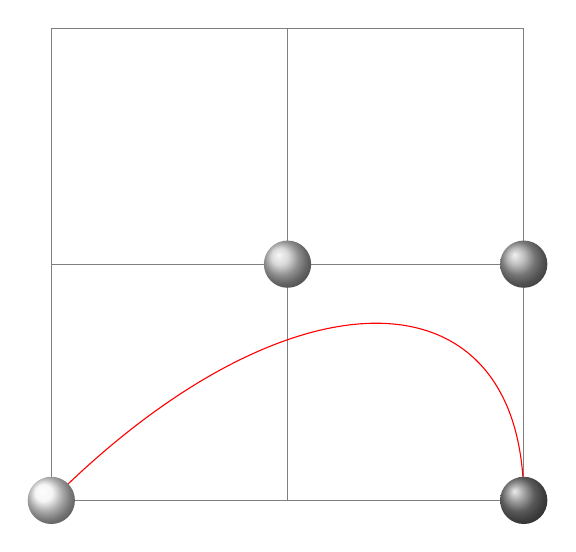
\begin{tikzpicture}[scale=3] 
\draw[help lines] (0,0) grid (2,2); 
\draw[color=red] (0,0) .. controls (1,1) and (2,1) .. (2,0); 
\shade[ball color=gray!10] (0,0) circle (0.1); 
\shade[ball color=gray!40] (1,1) circle (0.1); 
\shade[ball color=gray!70] (2,1) circle (0.1); 
\shade[ball color=gray] (2,0) circle (0.1); 
\end{tikzpicture}
\end{lstlisting}
\begin{center}
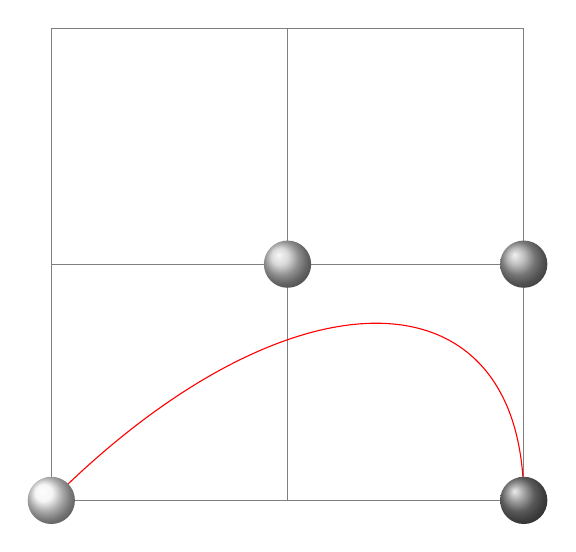
\begin{tikzpicture}[scale=3] 
\draw[help lines] (0,0) grid (2,2); 
\draw[color=red] (0,0) .. controls (1,1) and (2,1) .. (2,0); 
\shade[ball color=gray!10] (0,0) circle (0.1); 
\shade[ball color=gray!40] (1,1) circle (0.1); 
\shade[ball color=gray!70] (2,1) circle (0.1); 
\shade[ball color=gray] (2,0) circle (0.1); 
\end{tikzpicture}
\end{center}
\subsection{点的相对偏移}
tikz中有一个重要的概念,当前点,然后点可以通过当前点根据相对偏移来确定一个新的点。上面代码第9行的 ++ 符号和第10行的 + 符号都根据当前点然后进行了 $\Delta x$ 和 $\Delta y$ 的相对偏移从而确定了一个新的点。这两个符号的区别在于是不是更新当前点数据。++符号更新当前点,而+符号不更新。

++适合描述一连串逐渐变化的点,+适合描述多个点围绕着一个点变化的情况。
\begin{lstlisting}
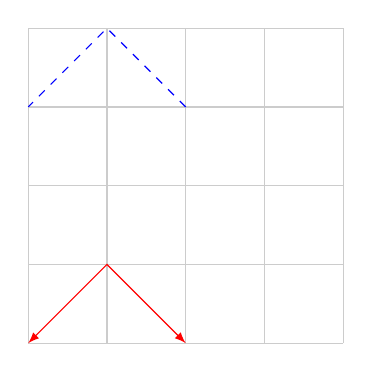
\begin{tikzpicture}[scale=1]
\draw[step=1,color=gray!40] (-2,-2) grid (2,2);
\draw[latex-latex, red] (0,-2) -- ++(-1,1) -- ++(-1,-1);
\draw[dashed, blue] (0,1) -- +(-1,1) -- +(-2,0);
\end{tikzpicture}
\end{lstlisting}
\begin{center}
	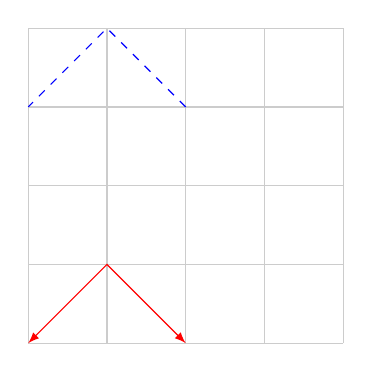
\begin{tikzpicture}[scale=1]
	\draw[step=1,color=gray!40] (-2,-2) grid (2,2);
	\draw[latex-latex, red] (0,-2) -- ++(-1,1) -- ++(-1,-1);
	\draw[dashed, blue] (0,1) -- +(-1,1) -- +(-2,0);
	\end{tikzpicture}
\end{center}

\subsection{node命令中点的定义}
tikz中的点也支持极坐标表示,(30:1cm),第一个参数是极座标里面的角度,第二个参数是半径。
\begin{lstlisting}
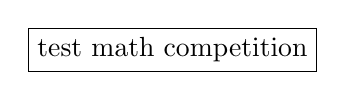
\begin{tikzpicture} 
\node (node001) at (0,2) [draw] {test math competition}; 
\end{tikzpicture}
\end{lstlisting}
\begin{center}
	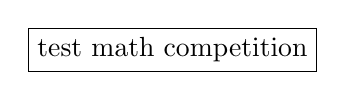
\begin{tikzpicture} 
	\node (node001) at (0,2) [draw] {test math competition}; 
	\end{tikzpicture}
\end{center}

从这里可以看到只要写上draw选项外面就会加上一个长方形,也就是shape的默认选项是rectangle。如果你不希望外面有长方形,不写draw选项即可。

这里通过node命令定义了一个点,node001,在(0,2)那里。后面是可以使用的。
\begin{lstlisting}
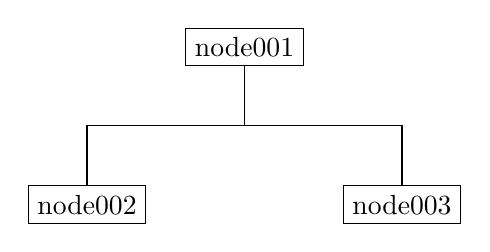
\begin{tikzpicture} 
\node (node001) at (0,2) [draw] {node001}; 
\node (node002) at (-2,0) [draw] {node002}; 
\node (node003) at (2,0) [draw] {node003}; 
\draw (node cs:name=node003,anchor=north) |- (0,1); 
\draw (node002.north) |- (0,1) -| (node cs:name=node001,anchor=south); 
\end{tikzpicture}
\end{lstlisting}
\begin{center}
	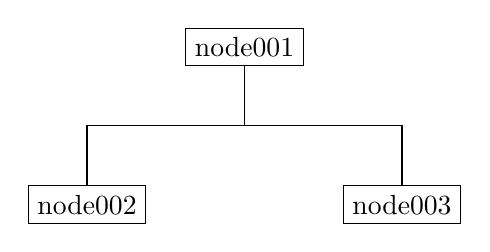
\begin{tikzpicture} 
	\node (node001) at (0,2) [draw] {node001}; 
	\node (node002) at (-2,0) [draw] {node002}; 
	\node (node003) at (2,0) [draw] {node003}; 
	\draw (node cs:name=node003,anchor=north) |- (0,1); 
	\draw (node002.north) |- (0,1) -| (node cs:name=node001,anchor=south); 
	\end{tikzpicture}
	
\end{center}

这里通过 node cs:name=node003 来获取之前那个node所在的点,然后通过 anchor=north 来定义那个node的接口在北边。除此之外的选项还有: south ,east ,west 。这里 |- 似乎是画垂直拐线的意思。上面的语法简写为可以node002.north。

此外还有 angle 选项控制node接口的开口角度。

\subsection{两个点定义出一个点}
\begin{lstlisting}
\begin{tikzpicture} 
\node (p1) at (30:1) {$p_1$} ; 
\node (p2) at (75:1) {$p_2$} ; 
\draw (-0.2,0) -- (1.2,0) node[right] (xline) {$q_1$}; 
\draw (2,-0.2) -- (2,1.2) node[above] (yline) {$q_2$}; 
\draw[->] (p1) -- (p1 |- xline); 
\end{tikzpicture}

\end{lstlisting}
\begin{center}
	\begin{tikzpicture} 
	\node (p1) at (30:1) {$p_1$} ; 
	\node (p2) at (75:1) {$p_2$} ; 
	\draw (-0.2,0) -- (1.2,0) node[right] (xline) {$q_1$}; 
	\draw (2,-0.2) -- (2,1.2) node[above] (yline) {$q_2$}; 
	\draw[->] (p1) -- (p1 |- xline); 
	\end{tikzpicture}
\end{center}

这种形式 (p1 |- xline) 表示取第一个点的$x$和第二个点的$y$组成一个新的点。如果是 (p1 -| xline) 表示取第二个点的$x$和第一个点的$y$组成一个新的点。

两个path的交点
\begin{lstlisting}
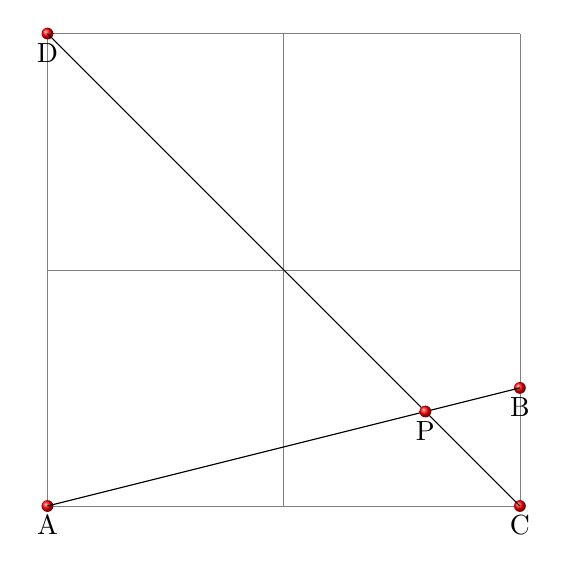
\begin{tikzpicture}[scale=3] 
\draw[help lines] (0,0) grid (2,2); 
\coordinate (A) at (0,0); 
\coordinate (B) at (2,0.5); 
\coordinate (C) at (2,0); 
\coordinate (D) at (0,2); 
\shade[ball color=red](A) circle (0.025) node[below] {A}; 
\shade[ball color=red](B) circle (0.025) node[below] {B}; 
\shade[ball color=red](C) circle (0.025) node[below] {C}; 
\shade[ball color=red](D) circle (0.025) node[below] {D}; 
\draw[name path=AB] (A) -- (B); \draw[name path=CD] (C) -- (D); 
\path[name intersections={of=AB and CD}] (intersection-1) coordinate (P); 
\shade[ball color=red](P) circle (0.025) node[below] {P}; 
\end{tikzpicture}
\end{lstlisting}
\begin{center}
	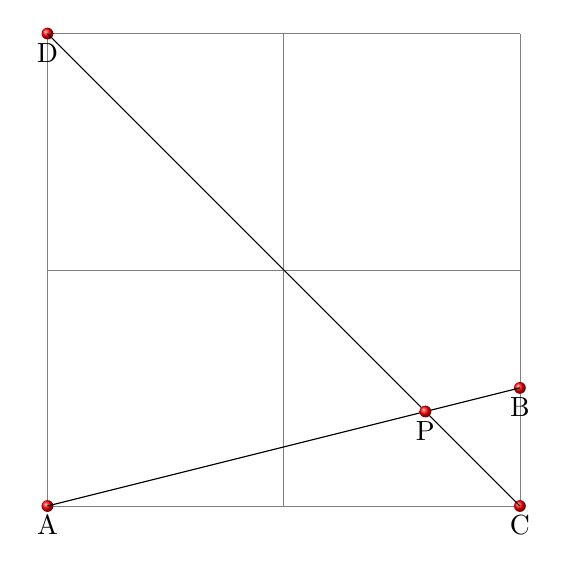
\begin{tikzpicture}[scale=3] 
	\draw[help lines] (0,0) grid (2,2); 
	\coordinate (A) at (0,0); 
	\coordinate (B) at (2,0.5); 
	\coordinate (C) at (2,0); 
	\coordinate (D) at (0,2); 
	\shade[ball color=red](A) circle (0.025) node[below] {A}; 
	\shade[ball color=red](B) circle (0.025) node[below] {B}; 
	\shade[ball color=red](C) circle (0.025) node[below] {C}; 
	\shade[ball color=red](D) circle (0.025) node[below] {D}; 
	\draw[name path=AB] (A) -- (B); \draw[name path=CD] (C) -- (D); 
	\path[name intersections={of=AB and CD}] (intersection-1) coordinate (P); 
	\shade[ball color=red](P) circle (0.025) node[below] {P}; 
	\end{tikzpicture}
\end{center}

这个例子用到了点的定义,点的标出,以及path交点的定义,要用到library: intersections 。有时候有些路径你不希望显示出来那么就用path命令来定义路径。

给新交点取名字:用 by 选项可以给画出来的交点取一个名字,默认的 intersection-1 之类的也可以使用。此外还可以加上选项:

\begin{Verbatim} 
\path[name intersections={of=D and E,by={[label=above:$C$]C,[label=below:$C'$]C'}}]; 
\end{Verbatim}
\section{圆(Circle Path)}
我们已经知道如何使用 tikz 在行内画图, 下面我们用以下代码在文中画出图
\begin{lstlisting}
\begin{tikzpicture} 
\draw[step=1,color=gray!40] (-2,-2) grid (2,2); 
\draw[->] (-3,0) -- (3,0); 
\draw[->] (0,-3) -- (0,3); 
\draw (0,0) circle (1);  
\end{tikzpicture}
\end{lstlisting}
\begin{center}
	\begin{tikzpicture} 
	\draw[step=1,color=gray!40] (-2,-2) grid (2,2); 
	\draw[->] (-3,0) -- (3,0); 
	\draw[->] (0,-3) -- (0,3); 
	\draw (0,0) circle (1);  
	\end{tikzpicture}
\end{center}

其中第一个点是圆中心,\lstinline{circle}表示画圆,第二个参数是半径大小.

\begin{lstlisting}
\begin{tikzpicture} 
\draw[step=1,color=gray!40] (-2,-2) grid (2,2); 
\draw[->] (-3,0) -- (3,0); 
\draw[->] (0,-3) -- (0,3); 
\draw (0,0) ellipse (1 and 0.5); 
\end{tikzpicture}
\end{lstlisting}
\begin{center}
	\begin{tikzpicture} 
	\draw[step=1,color=gray!40] (-2,-2) grid (2,2); 
	\draw[->] (-3,0) -- (3,0); 
	\draw[->] (0,-3) -- (0,3); 
	\draw (0,0) ellipse (1 and 0.5); 
	\end{tikzpicture}
\end{center}

这里第一个点是椭圆的中心点,ellipse表示画椭圆,后面参数两个值第一个是a也就是椭圆的半长轴,第二个是b也就是椭圆的半短轴。用法:
\begin{Verbatim} 
\draw[options] (x,y) circle (raidus);
\draw[options] (x,y) ellipse (x.raidus anda y.radius);
\end{Verbatim}

\begin{lstlisting}
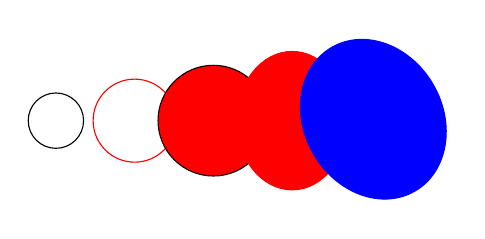
\begin{tikzpicture}
\draw (0,0) circle (10pt);
\draw[red] (1,0) circle (15pt);
\draw[fill=red] (2,0) circle (20pt);
\draw[red,fill=red] (3,0) ellipse (20pt and 25pt);
\filldraw[blue,rotate=30] (3.5,-2) ellipse (25pt and 30pt); % another way
\end{tikzpicture}

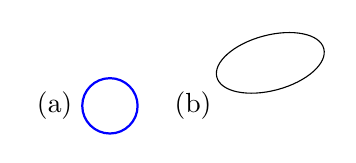
\begin{tikzpicture}
\draw (- 20pt,0) node [auto] {(a)};
\draw [thick ,blue ] (0pt ,0pt ) circle [radius =10 pt ] ;

\draw (30pt,0) node [auto] {(b)};
\draw [rotate =15] (60pt ,0) ellipse [x radius =20 pt , y radius =10 pt ];
\end{tikzpicture}
\tikz {\draw (0,0) circle (1);\fill [green](0,0) circle (1);}
\tikz \filldraw [red] (0,0) ellipse (2 and 1);
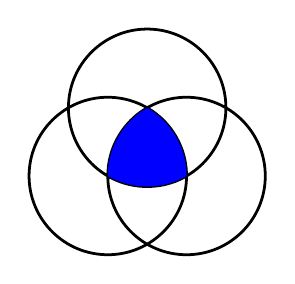
\begin{tikzpicture}[line width=1pt]
\draw (0,0)circle(1.0) (1,0)circle(1.0)
(60:1)circle(1.0);
\clip (0,0) circle (1.0);
\clip (1,0) circle (1.0);
\fill[blue] (60:1)circle(1.0);
\end{tikzpicture}
\begin{center}
\tikz {\draw (0,0)coordinate(D) node[below left=-0.5pt and -4pt]{$D$} --(0,1)coordinate(A) node[above left=-0.5pt and -4pt]{$A$}--(2,1)coordinate(B) node[above]{$B$} -- (1, 1) arc [start angle=90, end angle=180, radius=1] rectangle (2,1)--(0,0)-- (2, 0)coordinate(C) node[below]{$C$} ;
\fill [green](0, 0) -- (2, 1) -- (1, 1)arc [start angle=90, end angle=180, radius=1] -- cycle;
\clip (0,0) rectangle (2,1);
\draw (1,0) circle(1);
\draw (0,0) -- (2,0);}
\end{center}
\end{lstlisting}
\begin{center}
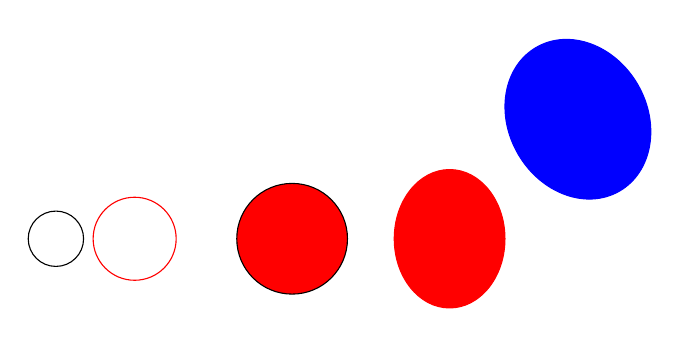
\begin{tikzpicture}
\draw (0,0) circle (10pt);
\draw[red] (1,0) circle (15pt);
\draw[fill=red] (3,0) circle (20pt);
\draw[red,fill=red] (5,0) ellipse (20pt and 25pt);
\filldraw[blue,rotate=30] (6.5,-2) ellipse (25pt and 30pt); % another way
\end{tikzpicture}
\end{center}
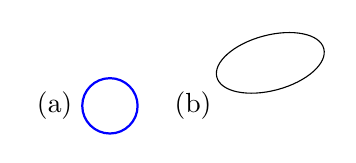
\begin{tikzpicture}
\draw (- 20pt,0) node [auto] {(a)};
\draw [thick ,blue ] (0pt ,0pt ) circle [radius =10 pt ] ;
\draw (30pt,0) node [auto] {(b)};
\draw [rotate =15] (60pt ,0) ellipse [x radius =20 pt , y radius =10 pt ];
\end{tikzpicture}
\tikz {\draw (0,0) circle (1);\fill [green](0,0) circle (1);}
\tikz \filldraw [red] (0,0) ellipse (2 and 1);
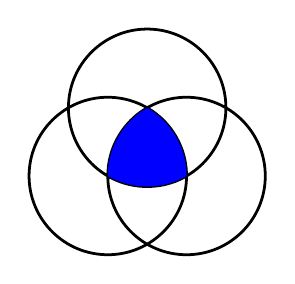
\begin{tikzpicture}[line width=1pt]
\draw (0,0)circle(1.0) (1,0)circle(1.0)
(60:1)circle(1.0);
\clip (0,0) circle (1.0);
\clip (1,0) circle (1.0);
\fill[blue] (60:1)circle(1.0);
\end{tikzpicture}
\begin{center}
\tikz {\draw (0,0)coordinate(D) node[below left=-0.5pt and -4pt]{$D$} --(0,1)coordinate(A) node[above left=-0.5pt and -4pt]{$A$}--(2,1)coordinate(B) node[above]{$B$} -- (1, 1) arc [start angle=90, end angle=180, radius=1] rectangle (2,1)--(0,0)-- (2, 0)coordinate(C) node[below]{$C$} ;
	\fill [green](0, 0) -- (2, 1) -- (1, 1)arc [start angle=90, end angle=180, radius=1] -- cycle;
	\clip (0,0) rectangle (2,1);
	\draw (1,0) circle(1);
	\draw (0,0) -- (2,0);}
\end{center}
\begin{lstlisting}
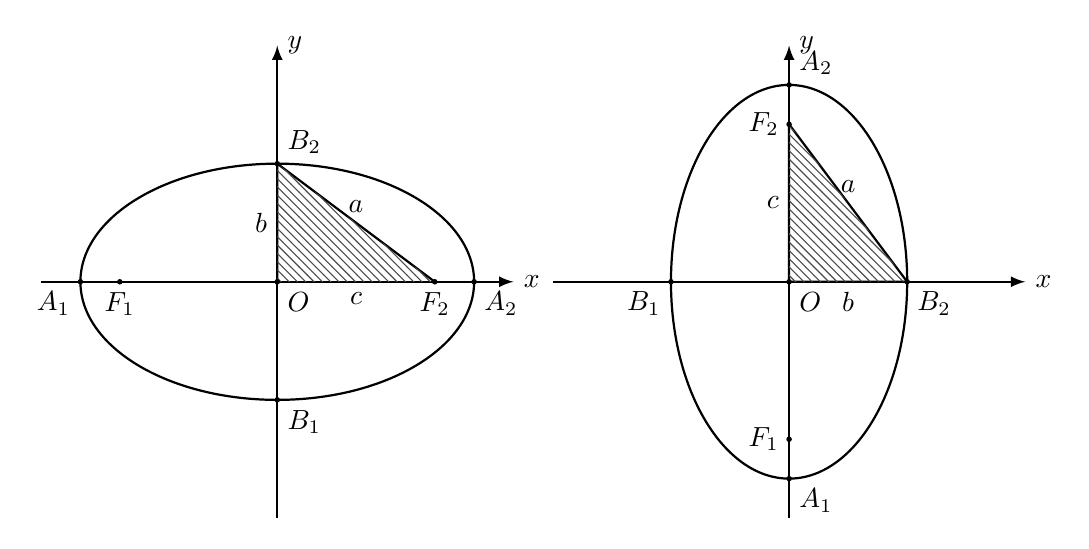
\begin{tikzpicture}[scale=0.5,thick]
\def\a{5}%长半轴
\def\b{3}%短半轴
\def\c{4}%焦半轴
\def\ptsize{2.0pt} %点的半径

%x 轴 和 y轴 
\path[name path=xaxis,thick,draw,->](-6,0)--(6,0) node[right] {$x$};
\path[name path=yaxis,thick,draw,->](0,-6)--(0,6) node[above,right] {$y$};
%x 轴 与 y 轴的交点 
\path [name intersections={of = xaxis and yaxis}];
\coordinate[label=below right:$O$] (O) at (intersection-1);
%画一个椭圆
\draw [name path = myellipse ] (intersection-1) ellipse (\a cm and \b cm);
%椭圆与x 轴交点
\path [name intersections={of = xaxis and myellipse}];
\coordinate[label=below right:$A_2$] (a2) at (intersection-1);
\coordinate[label=below left:$A_1$] (a1) at (intersection-2);
%椭圆与y 轴交点
\path [name intersections={of = yaxis and myellipse}];
\coordinate[label=above right:$B_2$] (b2) at (intersection-1);
\coordinate[label=below right:$B_1$] (b1) at (intersection-2);
%焦点
\coordinate[label=below :$F_1$] (f1) at (-\c,0);
\coordinate[label=below :$F_2$] (f2) at (\c,0);
%a b c 的几何意义
\draw (b2) --(f2) node[midway,above] {$a$};
\draw (b2) --(O) node[midway,left] {$b$};
\draw (O) --(f2) node[midway,below] {$c$};
%阴影部分填充
\fill [pattern =north west lines,pattern color = black!70](b2)--(O)--(f2)--cycle;
%画点
\foreach \p in {O,a1,a2,b1,b2,f1,f2}
\fill (\p) circle (\ptsize);
%在图像右侧再画一个焦点在y轴上的椭圆
\begin{scope}[xshift=13cm]
\path[name path=xaxis,thick,draw,->](-6,0)--(6,0) node[right] {$x$};
\path[name path=yaxis,thick,draw,->](0,-6)--(0,6) node[above,right] {$y$};
\path [name intersections={of = xaxis and yaxis}];
\coordinate[label=below right:$O$] (O) at (intersection-1);
%画一个椭圆
\draw [name path = myellipse ] (intersection-1) ellipse (\b cm and \a cm);

\path [name intersections={of = xaxis and myellipse}];
\coordinate[label=below right:$B_2$] (a2) at (intersection-1);
\coordinate[label=below left:$B_1$] (a1) at (intersection-2);

\path [name intersections={of = yaxis and myellipse}];
\coordinate[label=above right:$A_2$] (b2) at (intersection-1);
\coordinate[label=below right:$A_1$] (b1) at (intersection-2);

\coordinate[label=left :$F_1$] (f1) at (0,-\c);
\coordinate[label=left :$F_2$] (f2) at (0,\c);

\draw (a2) --(f2) node[midway,above] {$a$};
\draw (a2) --(O) node[midway,below] {$b$};
\draw (O) --(f2) node[midway,left] {$c$};

\fill [pattern =north west lines,pattern color = black!70](a2)--(O)--(f2)--cycle;

\foreach \p in {O,a1,a2,b1,b2,f1,f2}
\fill (\p) circle (\ptsize);

\end{scope}
\end{tikzpicture}
\end{lstlisting}
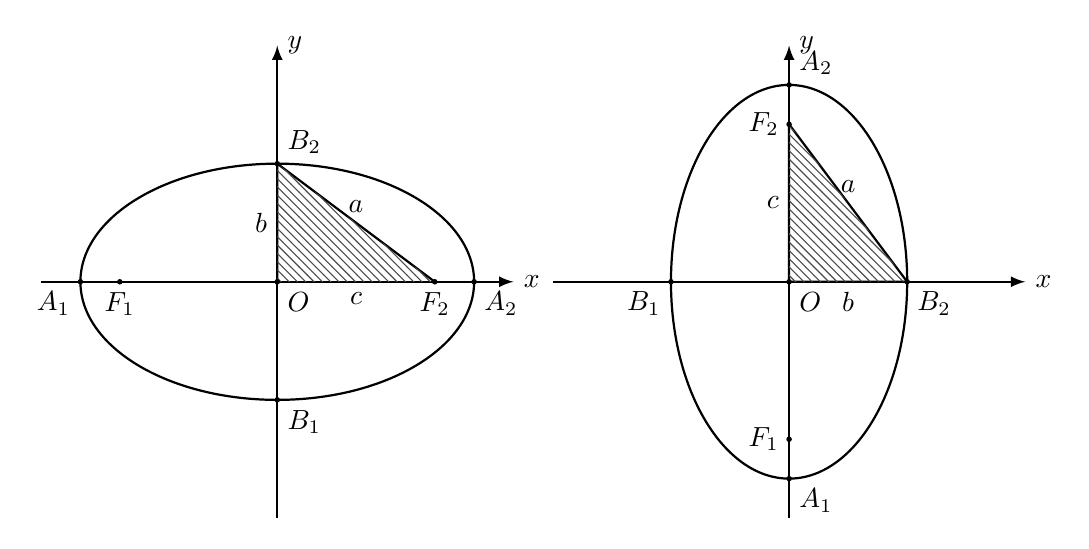
\begin{tikzpicture}[scale=0.5,thick]
\def\a{5}%长半轴
\def\b{3}%短半轴
\def\c{4}%焦半轴
\def\ptsize{2.0pt} %点的半径

%x 轴 和 y轴 
\path[name path=xaxis,thick,draw,->](-6,0)--(6,0) node[right] {$x$};
\path[name path=yaxis,thick,draw,->](0,-6)--(0,6) node[above,right] {$y$};
%x 轴 与 y 轴的交点 
\path [name intersections={of = xaxis and yaxis}];
\coordinate[label=below right:$O$] (O) at (intersection-1);
%画一个椭圆
\draw [name path = myellipse ] (intersection-1) ellipse (\a cm and \b cm);
%椭圆与x 轴交点
\path [name intersections={of = xaxis and myellipse}];
\coordinate[label=below right:$A_2$] (a2) at (intersection-1);
\coordinate[label=below left:$A_1$] (a1) at (intersection-2);
%椭圆与y 轴交点
\path [name intersections={of = yaxis and myellipse}];
\coordinate[label=above right:$B_2$] (b2) at (intersection-1);
\coordinate[label=below right:$B_1$] (b1) at (intersection-2);
%焦点
\coordinate[label=below :$F_1$] (f1) at (-\c,0);
\coordinate[label=below :$F_2$] (f2) at (\c,0);
%a b c 的几何意义
\draw (b2) --(f2) node[midway,above] {$a$};
\draw (b2) --(O) node[midway,left] {$b$};
\draw (O) --(f2) node[midway,below] {$c$};
%阴影部分填充
\fill [pattern =north west lines,pattern color = black!70](b2)--(O)--(f2)--cycle;
%画点
\foreach \p in {O,a1,a2,b1,b2,f1,f2}
\fill (\p) circle (\ptsize);
%在图像右侧再画一个焦点在y轴上的椭圆
\begin{scope}[xshift=13cm]
\path[name path=xaxis,thick,draw,->](-6,0)--(6,0) node[right] {$x$};
\path[name path=yaxis,thick,draw,->](0,-6)--(0,6) node[above,right] {$y$};
\path [name intersections={of = xaxis and yaxis}];
\coordinate[label=below right:$O$] (O) at (intersection-1);
%画一个椭圆
\draw [name path = myellipse ] (intersection-1) ellipse (\b cm and \a cm);

\path [name intersections={of = xaxis and myellipse}];
\coordinate[label=below right:$B_2$] (a2) at (intersection-1);
\coordinate[label=below left:$B_1$] (a1) at (intersection-2);

\path [name intersections={of = yaxis and myellipse}];
\coordinate[label=above right:$A_2$] (b2) at (intersection-1);
\coordinate[label=below right:$A_1$] (b1) at (intersection-2);

\coordinate[label=left :$F_1$] (f1) at (0,-\c);
\coordinate[label=left :$F_2$] (f2) at (0,\c);

\draw (a2) --(f2) node[midway,above] {$a$};
\draw (a2) --(O) node[midway,below] {$b$};
\draw (O) --(f2) node[midway,left] {$c$};

\fill [pattern =north west lines,pattern color = black!70](a2)--(O)--(f2)--cycle;

\foreach \p in {O,a1,a2,b1,b2,f1,f2}
\fill (\p) circle (\ptsize);

\end{scope}

\end{tikzpicture}
\begin{lstlisting}
\begin{tikzpicture}
\draw(3,-1) coordinate (A) node[right] {A}
-- (0,0) coordinate (B) node[left] {B}
-- (2,2) coordinate (C) node[above right] {C}
pic["$60\circ$", draw=orange, <->, angle eccentricity=1.2, angle radius=1cm]
{angle=A--B--C};
\end{tikzpicture}

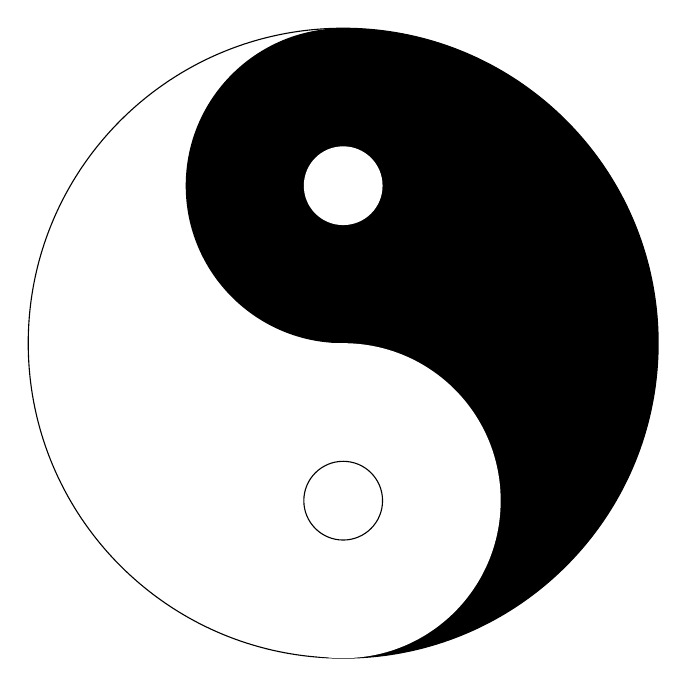
\begin{tikzpicture}
\draw(0,0) circle(4cm);  %画一个4cm的圆圈
%把圆的右半边填黑
\begin{scope}
\clip(0,0) circle(4cm);
\fill[black] (0,-4) rectangle (4,4);
\end{scope}
%填黑八卦图左边的半圆
\begin{scope}
\clip(0,2) circle(2cm);
\fill[black] (-4,0) rectangle (4,4);
\end{scope}
%填白八卦图右边的半圆
\begin{scope}
\clip(0,-2) circle(2cm);
\fill[white] (-4,0) rectangle (4,-4);
\end{scope}
%把黑色部分的小圆圈填为白色
\begin{scope}
\clip(0,2) circle(0.5cm);
\fill[white] (-4,0) rectangle (4,4);
\end{scope}
%绘制下面的白色圆圈
\draw(0,-2) circle(0.5cm);
\end{tikzpicture}
\end{lstlisting}
\begin{tikzpicture}
\draw(3,-1) coordinate (A) node[right] {A}
-- (0,0) coordinate (B) node[left] {B}
-- (2,2) coordinate (C) node[above right] {C}
pic["$60\circ$", draw=orange, <->, angle eccentricity=1.2, angle radius=1cm]
{angle=A--B--C};
\end{tikzpicture}
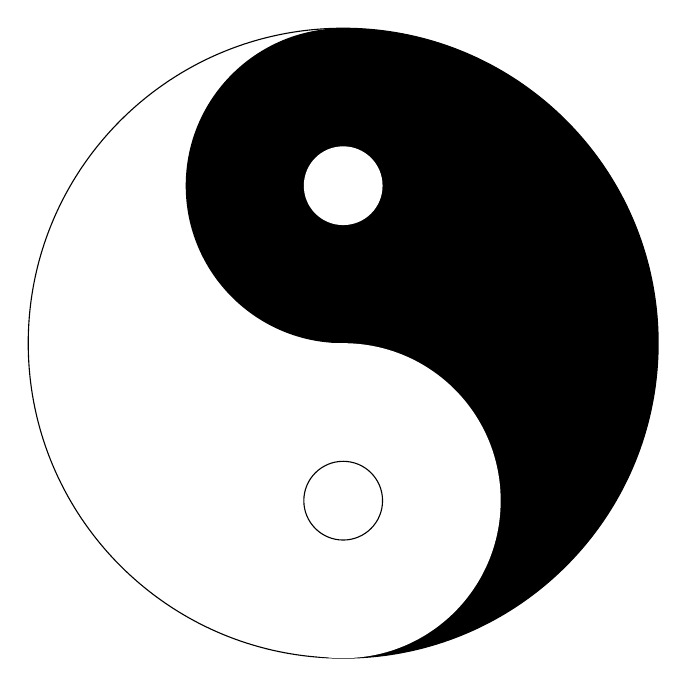
\begin{tikzpicture}
\draw(0,0) circle(4cm);  %画一个4cm的圆圈
%把圆的右半边填黑
\begin{scope}
\clip(0,0) circle(4cm);
\fill[black] (0,-4) rectangle (4,4);
\end{scope}
%填黑八卦图左边的半圆
\begin{scope}
\clip(0,2) circle(2cm);
\fill[black] (-4,0) rectangle (4,4);
\end{scope}
%填白八卦图右边的半圆
\begin{scope}
\clip(0,-2) circle(2cm);
\fill[white] (-4,0) rectangle (4,-4);
\end{scope}
%把黑色部分的小圆圈填为白色
\begin{scope}
\clip(0,2) circle(0.5cm);
\fill[white] (-4,0) rectangle (4,4);
\end{scope}
%绘制下面的白色圆圈
\draw(0,-2) circle(0.5cm);
\end{tikzpicture}
\begin{lstlisting}
\begin{center}
\begin{tikzpicture}
\foreach \x in {0,1,...,10} {
\node[draw, circle, inner sep=0pt, minimum size=\x mm] {};
}
\foreach \a/\x/\y in {1/orange/八一杯, 2/teal/团子杯, 3/magenta/熊赛} {
\node[circle, minimum size=2*\a mm, draw=\x!90, fill=\x!30, text=\x!70] at (2*\a, 0) {\y};
}
\end{tikzpicture}

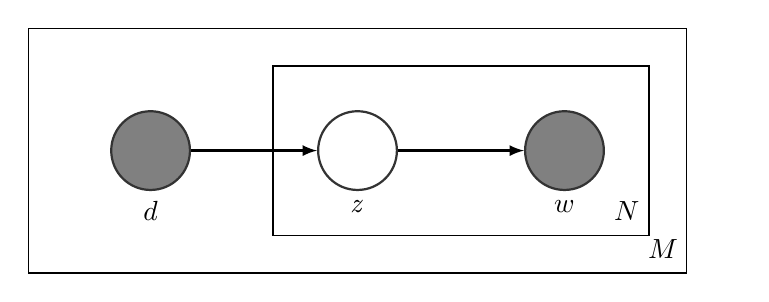
\begin{tikzpicture}
\tikzstyle{main}=[circle, minimum size = 10mm, thick, draw =black!80, node distance = 16mm]
\tikzstyle{connect}=[-latex, thick]
\tikzstyle{box}=[rectangle, draw=black!100]
\node[main, fill = white!100] (z) [label=below:\emph{z}] { };
\node[main, fill = black!50] (d) [left=of z,label=below:$d$] { };
\node[main, fill = black!50] (w) [right=of z,label=below:$w$] {};
\path (d) edge [connect] (z)
(z) edge [connect] (w);
\node[rectangle, inner sep=0mm, fit= (z) (w),label=below right:$N$, xshift=13mm] {};
\node[rectangle, inner sep=5.6mm,draw=black!100, fit= (z) (w)] {};
\node[rectangle, inner sep=4.8mm, fit= (z) (w),label=below right:$M$, xshift=12.5mm] {};
\node[rectangle, inner sep=10.4mm, draw=black!100, fit = (d) (z) (w)] {};
\end{tikzpicture}
\end{center}
\end{lstlisting}
\begin{center}
	\begin{tikzpicture}
	\foreach \x in {0,1,...,10} {
		\node[draw, circle, inner sep=0pt, minimum size=\x mm] {};
	}
	\foreach \a/\x/\y in {1/orange/八一杯, 2/teal/团子杯, 3/magenta/熊赛} {
		\node[circle, minimum size=2*\a mm, draw=\x!90, fill=\x!30, text=\x!70] at (2*\a, 0) {\y};
	}
\end{tikzpicture}
	
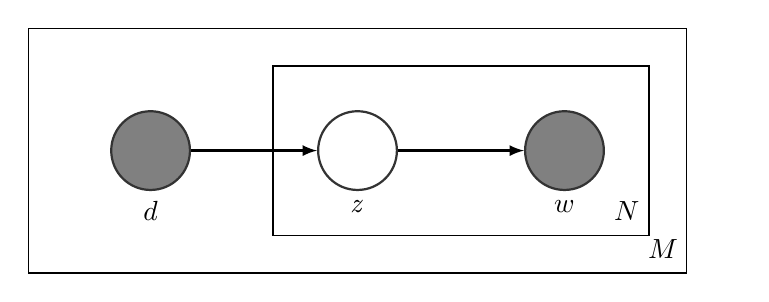
\begin{tikzpicture}
	\tikzstyle{main}=[circle, minimum size = 10mm, thick, draw =black!80, node distance = 16mm]
	\tikzstyle{connect}=[-latex, thick]
	\tikzstyle{box}=[rectangle, draw=black!100]
	\node[main, fill = white!100] (z) [label=below:\emph{z}] { };
	\node[main, fill = black!50] (d) [left=of z,label=below:$d$] { };
	\node[main, fill = black!50] (w) [right=of z,label=below:$w$] {};
	\path (d) edge [connect] (z)
	(z) edge [connect] (w);
	\node[rectangle, inner sep=0mm, fit= (z) (w),label=below right:$N$, xshift=13mm] {};
	\node[rectangle, inner sep=5.6mm,draw=black!100, fit= (z) (w)] {};
	\node[rectangle, inner sep=4.8mm, fit= (z) (w),label=below right:$M$, xshift=12.5mm] {};
	\node[rectangle, inner sep=10.4mm, draw=black!100, fit = (d) (z) (w)] {};
\end{tikzpicture}
\end{center}
\section{矩形与多边形(Rectangle Path)}
画正方形或矩形使用关键字 rectangle ,左下角和右上角坐标控制整个矩形的形状。如果将矩形旋转,则旋转角度以右下角坐标为轴心,逆时针方向旋转。用法如下:
\begin{verbatim}
 	\draw[options] (x1,y1) rectangle (x2,y2);
	\draw[options] (x,y) rectangle +(width,height);
\end{verbatim}
\begin{lstlisting}
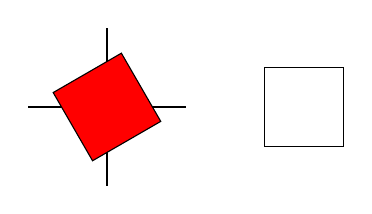
\begin{tikzpicture}
\draw (-1,0) -- (1,0);
\draw (0,-1) -- (0,1);
\draw[rotate=30, fill=red] (-0.5,-0.5) rectangle (0.5,0.5);
\draw (2,-0.5) rectangle +(1,1);
\end{tikzpicture}
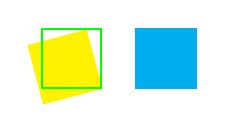
\begin{tikzpicture}[scale=1.5]
% 第一个坐标为左下角,第二个坐标为右上角。
\filldraw [thick ,cyan ] (0.3,0) rectangle (0.8, 0.5);
% 旋转角度以右下角坐标为轴心 ,逆时针旋转。
\filldraw [thick ,yellow ,rotate =15] (- 0.5,0) rectangle (0,0.5);
\draw [thick ,green ] (- 0.5,0) rectangle (0,0.5);
\end{tikzpicture}
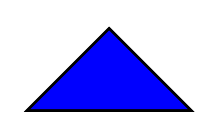
\begin{tikzpicture}[line width=2pt]
\draw (0,0) --(1,1) --(2,0) --cycle;
\fill[blue] (0,0) --(1,1) --(2,0) --cycle;
\end{tikzpicture}
\tikz \draw (0,0) rectangle (2,1);
\tikz \draw [step=0.5] (0,0) grid (3,2);
\tikz {\draw (0,0) circle (1);\fill [green](0,0) circle (1);}
\end{lstlisting}
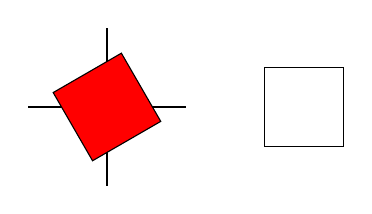
\begin{tikzpicture}
\draw (-1,0) -- (1,0);
\draw (0,-1) -- (0,1);
\draw[rotate=30, fill=red] (-0.5,-0.5) rectangle (0.5,0.5);
\draw (2,-0.5) rectangle +(1,1);
\end{tikzpicture}
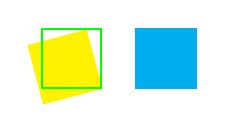
\begin{tikzpicture}[scale=1.5]
% 第一个坐标为左下角,第二个坐标为右上角。
\filldraw [thick ,cyan ] (0.3,0) rectangle (0.8, 0.5);
% 旋转角度以右下角坐标为轴心 ,逆时针旋转。
\filldraw [thick ,yellow ,rotate =15] (- 0.5,0) rectangle (0,0.5);
\draw [thick ,green ] (- 0.5,0) rectangle (0,0.5);
\end{tikzpicture}
\begin{tikzpicture}[line width=2pt]
\draw (0,0) --(1,1) --(2,0) --cycle;
\fill[blue] (0,0) --(1,1) --(2,0) --cycle;
\end{tikzpicture}
\tikz \draw (0,0) rectangle (2,1);
\tikz \draw [step=0.5] (0,0) grid (3,2);
\tikz {\draw (0,0) circle (1);\fill [green](0,0) circle (1);}
\begin{lstlisting}
\begin{tikzpicture}[scale=2]
\draw[step=1,color=gray!40] (-2,-2) grid (2,2);
\draw[color=red] (-1,-1) rectangle (1,1);
\end{tikzpicture}
\end{lstlisting}
\begin{center}
	\begin{tikzpicture}[scale=2]
	\draw[step=1,color=gray!40] (-2,-2) grid (2,2);
	\draw[color=red] (-1,-1) rectangle (1,1);
	\end{tikzpicture}
\end{center}

这里使用了可选项 color=red 来控制线条的颜色,然后画长方形的第一个点是左底点,rectangle表示画长方形,第二个点表示右顶点。如果想要放大图形,可在tikzpicture环境后面跟上可选项 [scale=2] ,即将图形放大两倍。
\begin{lstlisting}
\begin{tikzpicture}
\draw (0,0) circle (4) ;
\coordinate (O) at (0,0);
\shade[ball color=red](O) circle (0.1) node[below] {O};
\def\n{5}
\pgfmathsetmacro\i{\n-1}
\foreach \x in {0,...,\i}
{
	\def\pointname{\x}
	\coordinate (\pointname) at ($(0,0) +(\x*360/\n:4cm)$)  ;
	\shade[ball color=red](\pointname) circle (0.05) node[below] {\small \x};
}

\draw (0)
\foreach \x in {0,...,\i}
{ -- (\x) } -- cycle;

\end{tikzpicture}
\end{lstlisting}
\begin{center}
\begin{tikzpicture}
\draw (0,0) circle (4) ;
\coordinate (O) at (0,0);
\shade[ball color=red](O) circle (0.1) node[below] {O};
\def\n{5}
\pgfmathsetmacro\i{\n-1}
\foreach \x in {0,...,\i}
{
\def\pointname{\x}
\coordinate (\pointname) at ($(0,0) +(\x*360/\n:4cm)$)  ;
\shade[ball color=red](\pointname) circle (0.05) node[below] {\small \x};
}

\draw (0)
\foreach \x in {0,...,\i}
{ -- (\x) } -- cycle;
\end{tikzpicture}
\end{center}
这个例子核心内容是批量定义点和点的运算,把这个弄懂了,后面tikz的核心大门就为你打开了,然后很多图形都可以用简洁的命令生成出来了。
\section{网格(Grid Path)}
网格主要用于辅助绘图,其中 help lines 是个不错的参数设置。其用法:
\begin{verbatim}
\draw[options] (x1,y1) grid (x2,y2); 
\end{verbatim}
\begin{lstlisting}
\begin{tikzpicture}
\draw[step=1.0cm, gray, very thin] (-1.4,-1.4) grid (1.4,1.4);
\draw (-1.5,0) -- (1.5,0);
\draw (0,-1.5) -- (0,1.5);
\draw (0,0) circle (1cm);
\draw[step=2pt] (0,0) grid (30pt,30pt);
\end{tikzpicture}
\end{lstlisting}
\begin{center}
 \begin{tikzpicture}
\draw[step=1.0cm, gray, very thin] (-1.4,-1.4) grid (1.4,1.4);
\draw (-1.5,0) -- (1.5,0);
\draw (0,-1.5) -- (0,1.5);
\draw (0,0) circle (1cm);
\draw[step=2pt] (0,0) grid (30pt,30pt);
\end{tikzpicture}
\end{center}
此外 step 用来控制网格之间的间距,可以color来设置网格的颜色,不过一般没那个必要。然后接下来第一个坐标点是网格的左底点,第二个坐标点是网格的右定点。
\begin{lstlisting}
\begin{tikzpicture} 
\draw[help lines] ( -5,-5 ) grid ( 5, 5); 
\end{tikzpicture}
\end{lstlisting}
\begin{center}
	\begin{tikzpicture} 
	\draw[help lines] ( -5,-5 ) grid ( 5, 5); 
	\end{tikzpicture}
\end{center}

我们看到tikz的每一条命令最后都要跟一个分号";"。
\section{直线(Straight Path)}
直线就是两个坐标点相连,中间 -- 符号表示直线的意思。用法如下:
\begin{verbatim}
\draw[options] (x1,y1) -- (x2,y2) -- (x3,y3);
\end{verbatim}
\begin{lstlisting}
\begin{tikzpicture}
\draw (-1.5,0) -- (1.5,0) -- (0,-1.5) -- (0,1.5);
\draw[thick, rounded corners=10pt] (0,0) -- (0,2) -- (1,3.25) -- 
(2,2) -- (2,0) -- (0,2) -- (2,2) -- (0,0) -- (2,0);
\end{tikzpicture}
\end{lstlisting}
\begin{center}
\begin{tikzpicture}
\draw (-1.5,0) -- (1.5,0) -- (0,-1.5) -- (0,1.5);
\draw[thick, rounded corners=10pt] (0,0) -- (0,2) -- (1,3.25) -- 
(2,2) -- (2,0) -- (0,2) -- (2,2) -- (0,0) -- (2,0);
\end{tikzpicture}
\end{center}
之前网格是grid表示网格的意思。如果几个点用 -- 符号连接起来,表示这几个点连着来画几条折线,有多个画直线命令依次执行的意思。
\begin{lstlisting}
\begin{tikzpicture} 
\draw[help lines] ( -4,-4 ) grid (4,4); 
\draw[red] (-3,0) -- (3,0); 
\draw[red] (0,-3) -- (0,3); 
\end{tikzpicture}
\end{lstlisting}
\begin{center}
\begin{tikzpicture} 
\draw[help lines] ( -4,-4 ) grid (4,4); 
\draw[red] (-3,0) -- (3,0); 
\draw[red] (0,-3) -- (0,3); 
\end{tikzpicture}
\end{center}
如果在直线带上箭头,draw命令可以跟上可选项 \lstinline{->} ,这样直线的右端就有一个箭头了。此外还有: \lstinline{->>},\lstinline {->|} , \lstinline{-to},\lstinline {-latex} ,\lstinline {-stealth} ,他们的效果从上到下依次演示如下:
\begin{lstlisting}
\begin{tikzpicture} 
\draw[->] (-3,3) -- (3,3); 
\draw[->>] (-3,2) -- (3,2); 
\draw[->|] (-3,1) -- (3,1); 
\draw[-to] (-3,0) -- (3,0); 
\draw[-latex] (-3,-1) -- (3,-1); 
\draw[-stealth] (-3,-2) -- (3,-2); 
\end{tikzpicture}
\end{lstlisting}
\begin{center}
\begin{tikzpicture} 
\draw[->] (-3,3) -- (3,3); 
\draw[->>] (-3,2) -- (3,2); 
\draw[->|] (-3,1) -- (3,1); 
\draw[-to] (-3,0) -- (3,0); 
\draw[-latex] (-3,-1) -- (3,-1); 
\draw[-stealth] (-3,-2) -- (3,-2); 
\end{tikzpicture}
\end{center}
\section{抛物线(Parabola Path)}
画实例用的抛物线使用关键字 parabola,用法如下:
\begin{verbatim}
\draw[options] (x1,y1) parabola (x2,y2);
\end{verbatim}

\tikz \draw (0,0) rectangle (1,1) (0,0) parabola (1,1);再画两个
\tikz \draw[x=0.2cm,y=0.2cm] (0,0) parabola bend (4,10) (6,6);\tikz \draw (0,0) sin (1,1) cos (2,0) sin (3,-1) cos (4,0);

第一个点 (0,0) 是起点,使用 sin画到第二点 (1,1) 。如果没有给出起点,那么 cos 会以 (1,1) 为起点,画到点 (2,0)。[x=1ex,y=1ex] 是表示在一个行距高度内,宽度为 1.57 倍的行距内画图。
section{箭头}
Tikz 默认的箭头有点难看,主要是因为它指的不精确。一个名字叫作“悄悄地 (stealth) ”的箭头。
\tikz{
	\draw [line width=1mm, -{Stealth[length=10mm, open]}]
	(0,0) -- (2,0);
	\draw [|<->|] (2,.6) -- node[above=1mm] {10mm} ++(-10mm,0);
}
\begin{tikzpicture}[>= stealth]
\draw [->, red] (0,0) arc [start angle =180, end angle=30,radius=1cm];
\draw [<<- ,very thick] (1,0) -- (1.5cm, 10pt) -- (2cm,0pt) -- (2.5cm,10pt);
\end{tikzpicture}

以及Arc Path的使用来绘制曲线,用法:
\begin{verbatim}
\draw (x,y) arc (angle1:angle2:radius);
\draw (x,y) arc [start angle=angle1, end angle=angle2, radius=radius];
\draw (x,y) arc (angle1:angle2:x.radius and y.radius);
\draw (x,y) arc [start angle=angle1, end angle=angle2, x radius=rx, y radius=ry]
\end{verbatim}
\begin{lstlisting}
\begin{tikzpicture}
\draw (-1.5,0) -- (1.5,0);
\draw (0,-1.5) -- (0,1.5);
\draw (0.5,0) arc (0:120:0.5cm);
\draw (1,0) arc (0:315:1.75cm and 1cm);
\draw (-1,0) arc [start angle=180, end angle=120, radius=0.5cm];
% 以上不是推荐的方式
\end{tikzpicture}
\end{lstlisting}
\begin{center}
	\begin{tikzpicture}
	\draw (-1.5,0) -- (1.5,0);
	\draw (0,-1.5) -- (0,1.5);
	\draw (0.5,0) arc (0:120:0.5cm);
	\draw (1,0) arc (0:315:1.75cm and 1cm);
	\draw (-1,0) arc [start angle=180, end angle=120, radius=0.5cm];
	% 以上不是推荐的方式
	\end{tikzpicture}
\end{center}

正弦或余弦曲线使用关键字sin/cos,用法:
\begin{verbatim}
\draw[options] (x1,y1) sin (x2,y2);
\draw[options] (x1,y1) cos (x2,y2);
\end{verbatim} 
\begin{lstlisting}
 \begin{tikzpicture}
\draw[help lines] (-0.5,-1.5) grid (4.5,1.5);
\draw[red] (0,0) sin (1,1) cos (2,0) sin (3,-1) cos (4,0);
\draw[blue] (0,1) cos (1,0) sin (2,-1) cos (3,0) sin (4,1);
\end{tikzpicture}
\end{lstlisting}
\begin{center}
	 \begin{tikzpicture}
	\draw[help lines] (-0.5,-1.5) grid (4.5,1.5);
	\draw[red] (0,0) sin (1,1) cos (2,0) sin (3,-1) cos (4,0);
	\draw[blue] (0,1) cos (1,0) sin (2,-1) cos (3,0) sin (4,1);
	\end{tikzpicture}
\end{center}
\begin{lstlisting}
\begin{tikzpicture}[scale=1.6]%scale参数可以使得图形放大一定的倍数而本身的字体大小可以保持不变。
\def\iangle{120}
%画左边的圆
%scope环境里够成一整个区块,然后可以使这一整个区块进行平移。
\begin{scope}[xshift=-2cm]
\draw[->] (-1.2,0) --(1.2,0);
\draw[->] (0,-1.2) --(0,1.2);
\draw[thick] (0,0) circle(1cm);
\coordinate [label = \iangle:$P$] (P) at (\iangle:1);
\coordinate [label = below:$P0$] (P0) at (P |-0,0);
\draw (P)--(P0);
\draw (0,0)--(P);
\fill [fill = gray,fill opacity=0.2] (0,0)--(0:1) arc (0:\iangle:1)--cycle;
\filldraw [fill = gray,fill opacity=0.5] (0,0)--(0:0.3) arc (0:\iangle:0.3)--cycle;
\node [right] at (\iangle/2:0.3) {\ang{\iangle}};

\end{scope}
%画右边的正弦曲线
\draw[->] (0,0) --({rad(210)},0);
\draw[->] (0,-1.2) --(0,1.2);
\draw [thick,domain=0:rad(210)] plot (\x,{sin(\x r)}) node [right] {$\sin x$};

\foreach \t in {0,90,180}
{
\draw ({rad(\t)},-0.05)--({rad(\t)},0.05) ;
\node [below,outer sep =2pt ,font=\small , fill = white] at ({rad(\t)},0) {\ang{\t}};
}
\foreach \y in {-1,1}
{
\draw (-0.05,\y) -- (0.05,\y);
}
\coordinate [label=above:{$Q$}] (Q) at ({rad(\iangle)},{sin(\iangle)});
\coordinate [label=below:{$Q_0$}] (Q0) at (Q |- 0,0);
\draw (Q)--(Q0);
%左右相互连接
\draw[dashed] (P) --(Q);
\end{tikzpicture}
\end{lstlisting}
\begin{center}
	\begin{tikzpicture}[scale=1.6]%scale参数可以使得图形放大一定的倍数而本身的字体大小可以保持不变。
	\def\iangle{120}
	%画左边的圆
	%scope环境里够成一整个区块,然后可以使这一整个区块进行平移。
	\begin{scope}[xshift=-2cm]
	\draw[->] (-1.2,0) --(1.2,0);
	\draw[->] (0,-1.2) --(0,1.2);
	\draw[thick] (0,0) circle(1cm);
	\coordinate [label = \iangle:$P$] (P) at (\iangle:1);
	\coordinate [label = below:$P0$] (P0) at (P |-0,0);
	\draw (P)--(P0);
	\draw (0,0)--(P);
	\fill [fill = gray,fill opacity=0.2] (0,0)--(0:1) arc (0:\iangle:1)--cycle;
	\filldraw [fill = gray,fill opacity=0.5] (0,0)--(0:0.3) arc (0:\iangle:0.3)--cycle;
	\node [right] at (\iangle/2:0.3) {\ang{\iangle}};
	
	\end{scope}
	%画右边的正弦曲线
	\draw[->] (0,0) --({rad(210)},0);
	\draw[->] (0,-1.2) --(0,1.2);
	\draw [thick,domain=0:rad(210)] plot (\x,{sin(\x r)}) node [right] {$\sin x$};
	
	\foreach \t in {0,90,180}
	{
		\draw ({rad(\t)},-0.05)--({rad(\t)},0.05) ;
		\node [below,outer sep =2pt ,font=\small , fill = white] at ({rad(\t)},0) {\ang{\t}};
	}
	\foreach \y in {-1,1}
	{
		\draw (-0.05,\y) -- (0.05,\y);
	}
	\coordinate [label=above:{$Q$}] (Q) at ({rad(\iangle)},{sin(\iangle)});
	\coordinate [label=below:{$Q_0$}] (Q0) at (Q |- 0,0);
	\draw (Q)--(Q0);
	%左右相互连接
	\draw[dashed] (P) --(Q);
	\end{tikzpicture}
\end{center}
\section{添加文本(Add text)}
添加文字比较简单,在已知位置上用 node 标出文字即可。其用法:
\begin{verbatim}
\draw (x,y) node[options] {text};
\draw (x,y) node[options] {text};
\node[options] at (x,y) {text};
options: above,below,left,right, or anchor=north,south,west,east.
\end{verbatim}
\begin{lstlisting}
\begin{tikzpicture}[scale=2]
\draw[<->] (0,1) -- (0,0) -- (1,0);
\draw[fill] (0.5,0.5) circle (0.05);
\draw (0.5,0.5) node[above=10pt] {A} node[left=10pt] {L} 
node[below=10pt] {B} node[right=10pt] {R};
\draw (0.5,0.5) node[above left=2pt] {AL} node[below left=2pt] {BL} 
node[below right=2pt] {BR} node[above right=2pt] {AR};
\end{tikzpicture}
\begin{tikzpicture}[scale=2]
\draw[<->] (0,1) -- (0,0) -- (1,0);
\draw[fill] (0.5,0.5) circle (0.05);
\draw (0.5,0.5) node[anchor=north] {N} node[anchor=west] {W} 
node[anchor=south] {S} node[anchor=east] {E};
\draw (0.5,0.5) node[anchor=north west] {NW} node[anchor=south west] {SW} 
node[anchor=south east] {SE} node[anchor=north east] {NE};
\end{tikzpicture}
\end{lstlisting}
\begin{center}
	\begin{tikzpicture}[scale=2]
	\draw[<->] (0,1) -- (0,0) -- (1,0);
	\draw[fill] (0.5,0.5) circle (0.05);
	\draw (0.5,0.5) node[above=10pt] {A} node[left=10pt] {L} 
	node[below=10pt] {B} node[right=10pt] {R};
	\draw (0.5,0.5) node[above left=2pt] {AL} node[below left=2pt] {BL} 
	node[below right=2pt] {BR} node[above right=2pt] {AR};
	\end{tikzpicture}
	\begin{tikzpicture}[scale=2]
	\draw[<->] (0,1) -- (0,0) -- (1,0);
	\draw[fill] (0.5,0.5) circle (0.05);
	\draw (0.5,0.5) node[anchor=north] {N} node[anchor=west] {W} 
	node[anchor=south] {S} node[anchor=east] {E};
	\draw (0.5,0.5) node[anchor=north west] {NW} node[anchor=south west] {SW} 
	node[anchor=south east] {SE} node[anchor=north east] {NE};
	\end{tikzpicture}
\end{center}
\begin{lstlisting}
\begin{tikzpicture}
\draw (0,0) .. controls (6,1) and (9,1) .. 
node[near start,sloped,above] {near start} 
node {midway} 
node[very near end,sloped,below] {very near end} (12,0);
\end{tikzpicture}
\end{lstlisting}
\begin{center}
	\begin{tikzpicture}
	\draw (0,0) .. controls (6,1) and (9,1) .. 
	node[near start,sloped,above] {near start} 
	node {midway} 
	node[very near end,sloped,below] {very near end} (12,0);
	\end{tikzpicture}
\end{center}
\begin{verbatim}
\begin{tikzpicture}
\draw (0,0) node(a) [draw,align=center] {This is a test\\$a$ node} 
(1,1) node(b) [draw] {Node B};
\draw (a.north) |- (b.west);
\draw[color=red] (a.east) -| (2,1.5) -| (b.north);
\end{tikzpicture}
\end{verbatim}
\begin{center}
	\begin{tikzpicture}
	\draw (0,0) node(a) [draw,align=center] {This is a test\\$a$ node} 
	(1,1) node(b) [draw] {Node B};
	\draw (a.north) |- (b.west);
	\draw[color=red] (a.east) -| (2,1.5) -| (b.north);
	\end{tikzpicture}
\end{center}
\begin{lstlisting}
\begin{tikzpicture}[scale=2, >= stealth]
\draw[step=0.5cm,gray,very thin] (-1.4,-1.4) grid (1.4,1.4);
\filldraw[fill=green!20!white,draw=red!50!black] (0,0) -- (3mm,0mm)
arc [start angle=0, end angle=30, radius=3mm] -- cycle ;
\draw (2mm, 0.4mm) node {$\alpha$};
\draw[->] (-1.5,0) -- (1.5,0) coordinate (x axis);
\draw[->] (0,-1.5) -- (0,1.5) coordinate (y axis);
\draw (0,0) circle [radius=1cm];
\draw [red,very thick] (30:1cm) -- node[left=1pt,fill=white] {$\sin \alpha$} +(0,-0.5);
\draw [blue,very thick] (30:1cm) ++(0,-0.5) -- node[below=2pt,fill=white] {$\cos \alpha$} (0,0);
\draw [orange,very thick] (1,0) -- (1,{tan(30)}) node[right=1pt,fill=white]
{$\displaystyle \tan \alpha \color{black}=
\frac{{\color{red}\sin \alpha }}{\color{blue}\cos \alpha}$};
\draw (0,0) -- (1,{tan(30)});
\foreach \x/\xtext in {-1,-0.5/-\frac{1}{2}, 1}
\draw [very thick] (\x cm, -1pt) -- (\x cm, 1pt) node[anchor=north,fill=white] {$\xtext$};
\foreach \y in {-1,-0.5,0.5,1}
\draw [very thick] (-1pt,\y cm) -- (1pt,\y cm) node[anchor=east,fill=white] {$\y$};
\end{tikzpicture}
\end{lstlisting}
\begin{center}
	\begin{tikzpicture}[scale=2, >= stealth]
	\draw[step=0.5cm,gray,very thin] (-1.4,-1.4) grid (1.4,1.4);
	\filldraw[fill=green!20!white,draw=red!50!black] (0,0) -- (3mm,0mm)
	arc [start angle=0, end angle=30, radius=3mm] -- cycle ;
	\draw (2mm, 0.4mm) node {$\alpha$};
	\draw[->] (-1.5,0) -- (1.5,0) coordinate (x axis);
	\draw[->] (0,-1.5) -- (0,1.5) coordinate (y axis);
	\draw (0,0) circle [radius=1cm];
	\draw [red,very thick] (30:1cm) -- node[left=1pt,fill=white] {$\sin \alpha$} +(0,-0.5);
	\draw [blue,very thick] (30:1cm) ++(0,-0.5) -- node[below=2pt,fill=white] {$\cos \alpha$} (0,0);
	\draw [orange,very thick] (1,0) -- (1,{tan(30)}) node[right=1pt,fill=white]
	{$\displaystyle \tan \alpha \color{black}=
		\frac{{\color{red}\sin \alpha }}{\color{blue}\cos \alpha}$};
	\draw (0,0) -- (1,{tan(30)});
	\foreach \x/\xtext in {-1,-0.5/-\frac{1}{2}, 1}
	\draw [very thick] (\x cm, -1pt) -- (\x cm, 1pt) node[anchor=north,fill=white] {$\xtext$};
	\foreach \y in {-1,-0.5,0.5,1}
	\draw [very thick] (-1pt,\y cm) -- (1pt,\y cm) node[anchor=east,fill=white] {$\y$};
	\end{tikzpicture}
\end{center}

\section{添加样式(Add Styles)}
\textsf{Styles}是可用于组织图形绘制方式的预定义选项集。要全局定义样式,可以在文档开头使用\textbackslash tikzset命令,用法:
\begin{verbatim}
\tikzset{style_name./style={options}}
\end{verbatim}
\begin{lstlisting}
\tikzset{blue_thin_lines/.style={color=blue!50,very thin}}
\begin{tikzpicture}
\draw[step=0.5cm, blue_thin_lines] (0,0) grid (2,2);
\end{tikzpicture}
\end{lstlisting}
\tikzset{blue_thin_lines/.style={color=blue!50,very thin}}
\begin{center}
\begin{tikzpicture}
\draw[step=0.5cm, blue_thin_lines] (0,0) grid (2,2);
\end{tikzpicture}
\end{center}
为了在局部定义一个样式,我们使用一对方括号 ``[ ]''来定义图片开头的样式,用法:
\begin{verbatim}
[style_name/.style={options}]
\end{verbatim}
\begin{lstlisting}
\begin{tikzpicture}
[red_thick_lines/.style={color=red!50,very thick}];
\draw[step=0.5cm, red_thick_lines] (0,0) grid (2,2);
\end{tikzpicture}
\end{lstlisting}
\begin{center}
	\begin{tikzpicture}
	[red_thick_lines/.style={color=red!50,very thick}];
	\draw[step=0.5cm, red_thick_lines] (0,0) grid (2,2);
	\end{tikzpicture}
\end{center}
也可以分层定义样式,用法:
\begin{verbatim}
\tikzset{style_name1/.style={style_name2, options}}
\end{verbatim}
\begin{lstlisting}
\tikzset{green_help_lines/.style={help lines, color=green!90}}
\begin{tikzpicture}
\draw[step=0.5cm, green_help_lines] (0,0) grid (5,5);
\end{tikzpicture}
\end{lstlisting}
\begin{center}
	\tikzset{green_help_lines/.style={help lines, color=green!90}}
	\begin{tikzpicture}
	\draw[step=0.5cm, green_help_lines] (0,0) grid (5,5);
	\end{tikzpicture}
\end{center}
样式也可以与参数一起使用,用法:
\begin{verbatim}
 [style_name/.style={options},style_name/.default={options}]
\end{verbatim}
\begin{lstlisting}
\begin{tikzpicture}
[para_color/.style={help lines,color=#1!50}, para_color/.default=blue]
\draw[step=0.5cm, para_color] (0,0) grid (2,2);
\draw[step=0.5cm, para_color=red] (2,0) grid (4,2);
\end{tikzpicture}
\end{lstlisting}
\begin{center}
	\begin{tikzpicture}
	[para_color/.style={help lines,color=#1!50}, para_color/.default=blue]
	\draw[step=0.5cm, para_color] (0,0) grid (2,2);
	\draw[step=0.5cm, para_color=red] (2,0) grid (4,2);
	\end{tikzpicture}
\end{center}

预定义一个属性集合,到时候直接赋给相应的实体,TikZ本身就是个宏,因此它为我们提供了强大的属性定义功能,来看这段代码:
\begin{lstlisting}
\begin{tikzpicture}
[LNode/.style={circle,   draw=blue!50, fill=blue!20, very thick, minimum size=10mm}
\node[LNode] (n1) at (0, 0){$\int x \mathrm{d}x$};
\end{tikzpicture}
\end{lstlisting}
\begin{center}
	\begin{tikzpicture}
	[L1Node/.style={circle,  draw=blue!50, fill=blue!20, very thick, minimum size=50mm}
%	L2Node/.style={rectangle,draw=green!50,fill=green!20,very thick, minimum size=50mm}]
	\node[L1Node] (n1) at (0, 0){$\int_{a}^{b} f(x)\mathrm{d}x$};
%	\node[L2Node] (n2) at (2, 0){$n!$};
	\end{tikzpicture}
\end{center}
\section{Draw options and context}
\subsection{绘图选项}
有一些绘图选项可以用来控制颜色、厚度和线条类型。
\begin{itemize}
	\item 颜色: 
	blue \tikz \filldraw[blue] (0,0) rectangle (1.5em,1.5ex);, 
	black \tikz \filldraw[black] (0,0) rectangle (1.5em,1.5ex);, 
	brown \tikz \filldraw[brown] (0,0) rectangle (1.5em,1.5ex);, 
	cyan \tikz \filldraw[cyan] (0,0) rectangle (1.5em,1.5ex);, 
	gray \tikz \filldraw[gray] (0,0) rectangle (1.5em,1.5ex);, 
	green \tikz \filldraw[green] (0,0) rectangle (1.5em,1.5ex);, 
	lightgray \tikz \filldraw[lightgray] (0,0) rectangle (1.5em,1.5ex);, 
	lime \tikz \filldraw[lime] (0,0) rectangle (1.5em,1.5ex);, 
	magenta \tikz \filldraw[magenta] (0,0) rectangle (1.5em,1.5ex);, 
	orange \tikz \filldraw[orange] (0,0) rectangle (1.5em,1.5ex);, 
	pink \tikz \filldraw[pink] (0,0) rectangle (1.5em,1.5ex);, 
	purple \tikz \filldraw[purple] (0,0) rectangle (1.5em,1.5ex);, 
	red \tikz \filldraw[red] (0,0) rectangle (1.5em,1.5ex);, 
	yellow \tikz \filldraw[yellow] (0,0) rectangle (1.5em,1.5ex);, 
	teal \tikz \filldraw[teal] (0,0) rectangle (1.5em,1.5ex);, 
	violet \tikz \filldraw[violet] (0,0) rectangle (1.5em,1.5ex);, 
	white \tikz \draw[fill=white] (0,0) rectangle (1.5em,1.5ex);.\\
	注意:颜色是可以混合, 比如这种颜色命令 \verb|[blue!40!white]| 意味着$40\%$蓝色和$60\%$白色混合在一起。
	\item 厚度: 
	ultra thin \begin{tikzpicture} \filldraw[white] (0,0) rectangle (1em,1.5ex); \draw[ultra thin] (0,0.7ex) -- (1em,0.7ex);\end{tikzpicture}, 
	very thin \begin{tikzpicture} \filldraw[white] (0,0) rectangle (1em,1.5ex); \draw[very thin] (0,0.7ex) -- (1em,0.7ex);\end{tikzpicture}, 
	thin \begin{tikzpicture} \filldraw[white] (0,0) rectangle (1em,1.5ex); \draw[thin] (0,0.7ex) -- (1em,0.7ex);\end{tikzpicture}, 
	semithick \begin{tikzpicture} \filldraw[white] (0,0) rectangle (1em,1.5ex); \draw[semithick] (0,0.7ex) -- (1em,0.7ex);\end{tikzpicture}, 
	thick \begin{tikzpicture} \filldraw[white] (0,0) rectangle (1em,1.5ex); \draw[thick] (0,0.7ex) -- (1em,0.7ex);\end{tikzpicture}, 
	very thick \begin{tikzpicture} \filldraw[white] (0,0) rectangle (1em,1.5ex); \draw[very thick] (0,0.7ex) -- (1em,0.7ex);\end{tikzpicture}, 
	ultra thick \begin{tikzpicture} \filldraw[white] (0,0) rectangle (1em,1.5ex); \draw[ultra thick] (0,0.7ex) -- (1em,0.7ex);\end{tikzpicture}.\\
	注意: \verb![help lines]=[gray,very thin]!. 线厚度也可以通过\verb![line width]! 选择,例如 \verb![line width=0.5cm]!.
	\item 线型: 
	loosely dashed \begin{tikzpicture} \filldraw[white] (0,0) rectangle (1em,1.5ex); \draw[loosely dashed] (0,0.7ex) -- (1em,0.7ex);\end{tikzpicture},
	dashed \begin{tikzpicture} \filldraw[white] (0,0) rectangle (1em,1.5ex); \draw[dashed] (0,0.7ex) -- (1em,0.7ex);\end{tikzpicture},
	densely dashed \begin{tikzpicture} \filldraw[white] (0,0) rectangle (1em,1.5ex); \draw[densely dashed] (0,0.7ex) -- (1em,0.7ex);\end{tikzpicture},
	loosely dotted \begin{tikzpicture} \filldraw[white] (0,0) rectangle (1em,1.5ex); \draw[loosely dotted] (0,0.7ex) -- (1em,0.7ex);\end{tikzpicture},
	dotted \begin{tikzpicture} \filldraw[white] (0,0) rectangle (1em,1.5ex); \draw[dotted] (0,0.7ex) -- (1em,0.7ex);\end{tikzpicture},
	densely dotted \begin{tikzpicture} \filldraw[white] (0,0) rectangle (1em,1.5ex); \draw[densely dotted] (0,0.7ex) -- (1em,0.7ex);\end{tikzpicture}.
	\item 箭头: 
	\verb!<-! \begin{tikzpicture} \filldraw[white] (0,0) rectangle (1em,1.5ex); \draw[<-] (0,0.7ex) -- (1em,0.7ex);\end{tikzpicture},
	\verb!<<-! \begin{tikzpicture} \filldraw[white] (0,0) rectangle (1em,1.5ex); \draw[<<-] (0,0.7ex) -- (1em,0.7ex);\end{tikzpicture},
	\verb!<-|! \begin{tikzpicture} \filldraw[white] (0,0) rectangle (1em,1.5ex); \draw[<-|] (0,0.7ex) -- (1em,0.7ex);\end{tikzpicture},
	\verb!<<-|! \begin{tikzpicture} \filldraw[white] (0,0) rectangle (1em,1.5ex); \draw[<<-|] (0,0.7ex) -- (1em,0.7ex);\end{tikzpicture},
	\verb!->! \begin{tikzpicture} \filldraw[white] (0,0) rectangle (1em,1.5ex); \draw[->] (0,0.7ex) -- (1em,0.7ex);\end{tikzpicture},
	\verb!->>! \begin{tikzpicture} \filldraw[white] (0,0) rectangle (1em,1.5ex); \draw[->>] (0,0.7ex) -- (1em,0.7ex);\end{tikzpicture},
	\verb!|->! \begin{tikzpicture} \filldraw[white] (0,0) rectangle (1em,1.5ex); \draw[|->] (0,0.7ex) -- (1em,0.7ex);\end{tikzpicture},
	\verb!|->>! \begin{tikzpicture} \filldraw[white] (0,0) rectangle (1em,1.5ex); \draw[|->>] (0,0.7ex) -- (1em,0.7ex);\end{tikzpicture},
	\verb!<->! \begin{tikzpicture} \filldraw[white] (0,0) rectangle (1em,1.5ex); \draw[<->] (0,0.7ex) -- (1em,0.7ex);\end{tikzpicture},
	\verb!<<->>! \begin{tikzpicture} \filldraw[white] (0,0) rectangle (1em,1.5ex); \draw[<<->>] (0,0.7ex) -- (1em,0.7ex);\end{tikzpicture}.\\
	注意:你也可以添加\verb!>=stealth!到选项中,它可将箭头更改为'stealth-like'的样式。
\end{itemize}
用法如下:
\begin{verbatim}
 \draw[color, thickness, line type, arrow] (x1,y1) -- (x2,y2);
\end{verbatim}
\begin{lstlisting}
\begin{tikzpicture}
\draw[red, very thin, densely dashed, <-] (0,0) -- (0.9,0);
\draw[green, ultra thick, loosely dotted, |->] (1.1,0) -- (1.9,0);
\draw[blue, semithick, <->, >=stealth] (2.1,0) -- (2.9,0);
\draw[purple, line width=0.3cm] (3.1,0) -- (3.9,0);
\end{tikzpicture}
\end{lstlisting}
\begin{center}
\begin{tikzpicture}
\draw[red, very thin, densely dashed, <-] (0,0) -- (0.9,0);
\draw[green, ultra thick, loosely dotted, |->] (1.1,0) -- (1.9,0);
\draw[blue, semithick, <->, >=stealth] (2.1,0) -- (2.9,0);
\draw[purple, line width=0.3cm] (3.1,0) -- (3.9,0);
\end{tikzpicture}
\end{center}
\subsection{node树}
node结点不但可以用于添加标识,还可以来绘制树形图,下面看一个例子,两个可作个对比,后面对前加了个样式:
\begin{lstlisting}
\begin{tikzpicture}
	\node {root}
	child {node {a1}}
	child {node {a2}
	child {node {b1}}
	child {node {b2}}}
	child {node {a3}};
\end{tikzpicture}
\begin{tikzpicture}
[every node/.style={fill=blue!30,draw=blue!70,rounded corners},
edge from parent/.style={blue,thick,draw}]
	\node {root}
	child {node {a1}}
	child {node {a2}
	child {node {b1}}
	child {node {b2}}}
	child {node {a3}};
\end{tikzpicture}
\end{lstlisting}
\begin{center}
	\begin{tikzpicture}
	\node {root}
	child {node {a1}}
	child {node {a2}
		child {node {b1}}
		child {node {b2}}}
	child {node {a3}};
	\end{tikzpicture}
	\begin{tikzpicture}
	[every node/.style={fill=blue!30,draw=blue!70,rounded corners},
	edge from parent/.style={blue,thick,draw}]
	\node {root}
	child {node {a1}}
	child {node {a2}
		child {node {b1}}
		child {node {b2}}}
	child {node {a3}};
	\end{tikzpicture}
\end{center}
\begin{lstlisting}
\tikzset{place/.style={circle,draw=blue!50,fill=blue!20,
thick,inner sep=0pt,minimum size=6mm}}
\tikzset{transition/.style={rectangle,draw=black!50,
fill=black!20,thick,inner sep=0pt,minimum size=4mm}}
\tikzset{every label/.style=red}
\begin{tikzpicture}[bend angle=45]
\node[place] (waiting)  {};
\node[place] (critical) [below=of waiting] {};
\node[place](semaphore) [below=of critical,label=above:$s\le3$] {};
\node[transition](leave critical) [right=of critical]{};
\node[transition] (enter critical)[left=of critical]{};
\draw [->] (enter critical) to (critical);
\draw [->] (waiting) to [bend right] (enter critical);
\draw [->] (enter critical) to [bend right] (semaphore);
\draw [->] (semaphore) to [bend right] (leave critical);
\draw [->] (critical) to (leave critical);
\draw [->] (leave critical) to [bend right] (waiting);
\end{tikzpicture}
\end{lstlisting}
\tikzset{place/.style={circle,draw=blue!50,fill=blue!20,
		thick,inner sep=0pt,minimum size=6mm}}
\tikzset{transition/.style={rectangle,draw=black!50,
		fill=black!20,thick,inner sep=0pt,minimum size=4mm}}
\tikzset{every label/.style=red}
\begin{center}
\begin{tikzpicture}[bend angle=45]
\node[place] (waiting)  {};
\node[place] (critical) [below=of waiting] {};
\node[place](semaphore) [below=of critical,label=above:$s\le3$] {};
\node[transition](leave critical) [right=of critical]{};
\node[transition] (enter critical)[left=of critical]{};
\draw [->] (enter critical) to (critical);
\draw [->] (waiting) to [bend right] (enter critical);
\draw [->] (enter critical) to [bend right] (semaphore);
\draw [->] (semaphore) to [bend right] (leave critical);
\draw [->] (critical) to (leave critical);
\draw [->] (leave critical) to [bend right] (waiting);
\end{tikzpicture}
\end{center}
\subsection{scope环境}
scope环境就是作用域控制,一个局域环境,参数只影响内部,外部的参数也影响不进来,不过值得一提的是,定义的点外面也可以用。scope环境一个有用的特性的里面的clip命令不会影响到外面。其用法:
\begin{verbatim}
\begin{scope}[options]
% only apply graphic options inside this scope, but not to anything outside.
\end{scope}
\end{verbatim}
\begin{lstlisting}
\begin{tikzpicture}[ultra thick]
\draw (0,0) -- (0,1);
\begin{scope}[thin]
\draw (1,0) -- (1,1);
\end{scope}
\draw (2,0) -- (2,1);
\end{tikzpicture}
\end{lstlisting}
\begin{center}
	\begin{tikzpicture}[ultra thick]
	\draw (0,0) -- (0,1);
	\begin{scope}[thin]
	\draw (1,0) -- (1,1);
	\end{scope}
	\draw (2,0) -- (2,1);
	\end{tikzpicture}
\end{center}
\subsection{迭代语句}
\begin{lstlisting}
\begin{tikzpicture}
\draw[help lines] (0,0) grid (3,2);
\foreach \x in {0,1,...,4}
\draw[xshift=\x cm] (0,-1) -- (0,1);
\end{tikzpicture}
\end{lstlisting}
\begin{center}
	\begin{tikzpicture}
	\draw[help lines] (0,0) grid (3,2);
	\foreach \x in {0,1,...,4}
	\draw[xshift=\x cm] (0,-1) -- (0,1);
	\end{tikzpicture}
\end{center}


其中... 表示一直这样有规律下去生成迭代列表。迭代语句有很多用法,详见后面的具体例子。
\subsection{其它}
\begin{enumerate}
	\item 平移:xshift ,x坐标轴平移。 yshift ,y坐标轴平移。 rotate ,旋转 。 注意xshift默认的单位并不是cm,如果要单位是cm需要写出来;
	\begin{center}
		\begin{tikzpicture} 
		\draw[help lines] (0,0) grid (3,2); 
		\draw (0,0) -- (1,1); 
		\draw[red] (0,0) -- ([xshift=1cm] 1,1); 
		\end{tikzpicture}
	\end{center}
	\item 旋转:后面加上可选项 rotate=30 即可,意思是图形逆时针旋转30度;
	\begin{center}
		\begin{tikzpicture} 
		\draw (0,0)[rotate=30]  ellipse (2 and 1); 
		\end{tikzpicture}
	\end{center}
	\item 反对称:xscale=-1或者yscale=-1就刚好相对y轴或x轴反对称;
	\item 翻转:例子如下
	\begin{lstlisting}
	\begin{tikzpicture}
	\draw[help lines, step=0.5] (0,0) grid (7,1.5);
	\draw[red, very thick] (0,0) -- (0,0.5) 
	[shift={(4pt,2pt)}] (0,0) -- (0,0.5);
	\draw[red, very thick] (0.5,0) -- (0.5,0.5) 
	[shift={+(4pt,2pt)}] (0.5,0) -- (0.5,0.5);
	\draw[rotate=30,fill=blue] (1.5,-1) rectangle (2,-0.5);
	\draw[rotate around={60:(3,0.5)},fill=blue] (2.5,0.25) rectangle (3,0.75);
	\draw[xscale=1,yscale=1.1,fill=green] (4,0.5) circle (0.5);
	\draw[xslant=2,very thick] (5,0) -- (5.5,0.5) -- (5.5,0);
	\end{tikzpicture}
	\end{lstlisting}
	\begin{center}
		\begin{tikzpicture}
		\draw[help lines, step=0.5] (0,0) grid (7,1.5);
		\draw[red, very thick] (0,0) -- (0,0.5) 
		[shift={(4pt,2pt)}] (0,0) -- (0,0.5);
		\draw[red, very thick] (0.5,0) -- (0.5,0.5) 
		[shift={+(4pt,2pt)}] (0.5,0) -- (0.5,0.5);
		\draw[rotate=30,fill=blue] (1.5,-1) rectangle (2,-0.5);
		\draw[rotate around={60:(3,0.5)},fill=blue] (2.5,0.25) rectangle (3,0.75);
		\draw[xscale=1,yscale=1.1,fill=green] (4,0.5) circle (0.5);
		\draw[xslant=2,very thick] (5,0) -- (5.5,0.5) -- (5.5,0);
		\end{tikzpicture}
	\end{center}
	\item 循环并行:其用法
	\begin{verbatim}
	\foreach \variable in {list of values}{
	\commands ;
	\end{verbatim}
	\begin{lstlisting}
	\begin{tikzpicture}
	\foreach \x in {-0.5cm,0cm,0.5cm}{
	\draw[red,very thick] (\x,-5pt) -- (\x,5pt);
	}
	\foreach \y in {-0.5cm,0cm,0.5cm}{
	\draw[blue,very thick] (1cm,\y) -- (1.5cm,\y);
	}
	\foreach \x in {0,...,9}{
	\draw[green,very thick] (\x,-1) circle (0.4cm);
	}
	\foreach \x in {2,2.5,...,4}{
	\draw[purple,very thick] (\x cm,-3pt) -- (\x cm,3pt);
	}
	\end{tikzpicture}
	\end{lstlisting}
	\begin{center}
	\begin{tikzpicture}
	\foreach \x in {-0.5cm,0cm,0.5cm}{
		\draw[red,very thick] (\x,-5pt) -- (\x,5pt);
	}
	\foreach \y in {-0.5cm,0cm,0.5cm}{
		\draw[blue,very thick] (1cm,\y) -- (1.5cm,\y);
	}
	\foreach \x in {0,...,9}{
		\draw[green,very thick] (\x,-1) circle (0.4cm);
	}
	\foreach \x in {2,2.5,...,4}{
		\draw[purple,very thick] (\x cm,-3pt) -- (\x cm,3pt);
	}
	\end{tikzpicture}
		\end{center}
	\begin{lstlisting}
	 \begin{tikzpicture}
	\foreach \x in {1,2,...,5,7,8,...,12}{
	\foreach \y in {1,...,5}{
	\draw (\x,\y) +(-0.5,-0.5) rectangle +(0.5,0.5);
	\draw (\x,\y) node{\x,\y};
	}
	}
	\end{tikzpicture}
	\end{lstlisting}
	\begin{center}
	 \begin{tikzpicture}
	\foreach \x in {1,2,...,5,7,8,...,12}{
		\foreach \y in {1,...,5}{
			\draw (\x,\y) +(-0.5,-0.5) rectangle +(0.5,0.5);
			\draw (\x,\y) node{\x,\y};
		}
	}
	\end{tikzpicture}
	\begin{lstlisting}
	\begin{tikzpicture}
	[L1Node/.style={circle,   draw=blue!50, fill=blue!20, very thick, minimum size=10mm},
	L2Node/.style={rectangle,draw=green!50,fill=green!20,very thick, minimum size=10mm}]
	\foreach \x in {1,...,5}
	\node[L1Node] (w1_\x) at (2*\x, 0){$\int_\Omega x_\x$};
	\end{tikzpicture}
	\end{lstlisting}
	\begin{center}
		\begin{tikzpicture}
		[L1Node/.style={circle,   draw=blue!50, fill=blue!20, very thick, minimum size=20mm},
		L2Node/.style={rectangle,draw=green!50,fill=green!20,very thick, minimum size=10mm}]
		\foreach \x in {1,...,5}
		\node[L1Node] (w1_\x) at (2*\x, 0){$\int_\Omega x_\x\mathrm{d}x$};
		\end{tikzpicture}
	\end{center}
	\end{center}
	\item 确定路径:
	\begin{itemize}
		\item 线条:path路径是最基本的命令,draw命令等价于 \lstinline{\path[draw]} ,fill命令等价于 \lstinline{\path[fill]} ,filldraw命令等价于 \lstinline{\path[draw,fill]} ,其他clip,shade命令情况类似。
		\item 虚线和点线:线条除了之前说的dashed和dotted两种样式之外,还有loosely dashed,densely dashed和loosely dotted, densely dotted;
		\item 线条的粗细:其他选项还有 ultra thin , very thin, thin, semithick, very thick, ultra thick
			\begin{center}
		\begin{tikzpicture} 
		\draw [ultra thick] (0,1) -- (2,1); 
		\draw [thick] (0,0.5) -- (2,0.5); 
		\draw [thin] (0,0) -- (2,0); 
		\end{tikzpicture}
			\end{center}
		或者直接通过可选项line width来定义:
			\begin{center}
		\begin{tikzpicture} 
		\draw [line width=0.4pt] (0,0) -- (2,0); 
		\draw[red]  (0,1) -- (2,1); 
		\draw [line width=0.2cm] (4,.75) -- (5,.25); 
		\end{tikzpicture}	
			\end{center}
	\end{itemize}
\end{enumerate}
\section{pgfplots宏包}
pgfplots宏包真是太好了,有时甚至画一个基本的坐标轴都懒得动用其他宏包命令了,我可以直接调用一个axis环境和进行一些简单的优化即可。当然就作为坐标轴作图可能总是用pgfplots宏包可能会稍显单调,但如果要求不是特别高的确实用pgfplots宏包会基于坐标轴的各个图形非常的称心如意,比如下面两个例子直接画函数与根据数据点来绘制:
\begin{lstlisting}
\begin{tikzpicture} 
\begin{axis} 
\addplot {x^2}; 
\end{axis} 
\end{tikzpicture}
\begin{tikzpicture}
\begin{axis} 
\addplot coordinates  
{(0,0) 
(1,1) 
(2,3) 
(3,9)}; 
\end{axis}
\end{tikzpicture}
\end{lstlisting}
\begin{tikzpicture} 
\begin{axis} 
\addplot {x^2}; 
\end{axis} 
\end{tikzpicture}
\begin{tikzpicture}
\begin{axis} 
\addplot coordinates  
{(0,0) 
	(1,1) 
	(2,3) 
	(3,9)}; 
\end{axis}
\end{tikzpicture}
\begin{lstlisting}
\begin{tikzpicture}
\begin{axis}
\addplot[color=red]{exp(x)};
\end{axis}
\end{tikzpicture}
%Here ends the furst plot
\hskip 5pt
%Here begins the 3d plot
\begin{tikzpicture}
\begin{axis}
\addplot3[
surf,
]
{exp(-x^2-y^2)*x};
\end{axis}
\end{tikzpicture}
\end{lstlisting}
\begin{tikzpicture}
\begin{axis}
\addplot[color=red]{exp(x)};
\end{axis}
\end{tikzpicture}
%Here ends the furst plot
\hskip 5pt
%Here begins the 3d plot
\begin{tikzpicture}
\begin{axis}
\addplot3[
surf,
]
{exp(-x^2-y^2)*x};
\end{axis}
\end{tikzpicture}
\begin{lstlisting}
\begin{tikzpicture}
\begin{axis}[
axis lines = left,
xlabel = $x$,
ylabel = {$f(x)$},
]
%Below the red parabola is defined
\addplot [
domain=-10:10, 
samples=100, 
color=red,
]
{x^2 - 2*x - 1};
\addlegendentry{$x^2 - 2x - 1$}
%Here the blue parabloa is defined
\addplot [
domain=-10:10, 
samples=100, 
color=blue,
]
{x^2 + 2*x + 1};
\addlegendentry{$x^2 + 2x + 1$}

\end{axis}
\end{tikzpicture}
\end{lstlisting}
\begin{center}
\begin{tikzpicture}
\begin{axis}[
axis lines = left,
xlabel = $x$,
ylabel = {$f(x)$},
]
%Below the red parabola is defined
\addplot [
domain=-10:10, 
samples=100, 
color=red,
]
{x^2 - 2*x - 1};
\addlegendentry{$x^2 - 2x - 1$}
%Here the blue parabloa is defined
\addplot [
domain=-10:10, 
samples=100, 
color=blue,
]
{x^2 + 2*x + 1};
\addlegendentry{$x^2 + 2x + 1$}

\end{axis}
\end{tikzpicture}
\end{center}
\begin{lstlisting}
\begin{tikzpicture}
\begin{axis}[
title={Temperature dependence of CuSO$_4\cdot$5H$_2$O solubility},
xlabel={Temperature [\textcelsius]},
ylabel={Solubility [g per 100 g water]},
xmin=0, xmax=100,
ymin=0, ymax=120,
xtick={0,20,40,60,80,100},
ytick={0,20,40,60,80,100,120},
legend pos=north west,
ymajorgrids=true,
grid style=dashed,
]

\addplot[
color=blue,
mark=square,
]
coordinates {
(0,23.1)(10,27.5)(20,32)(30,37.8)(40,44.6)(60,61.8)(80,83.8)(100,114)
};
\legend{CuSO$_4\cdot$5H$_2$O}

\end{axis}
\end{tikzpicture}
\end{lstlisting}
\begin{center}
\begin{tikzpicture}
\begin{axis}[
title={Temperature dependence of CuSO$_4\cdot$5H$_2$O solubility},
xlabel={Temperature [\textcelsius]},
ylabel={Solubility [g per 100 g water]},
xmin=0, xmax=100,
ymin=0, ymax=120,
xtick={0,20,40,60,80,100},
ytick={0,20,40,60,80,100,120},
legend pos=north west,
ymajorgrids=true,
grid style=dashed,
]

\addplot[
color=blue,
mark=square,
]
coordinates {
	(0,23.1)(10,27.5)(20,32)(30,37.8)(40,44.6)(60,61.8)(80,83.8)(100,114)
};
\legend{CuSO$_4\cdot$5H$_2$O}

\end{axis}
\end{tikzpicture}
\end{center}
\begin{lstlisting}
\begin{tikzpicture}
\begin{axis}[
x tick label style={
/pgf/number format/1000 sep=},
ylabel=Year,
enlargelimits=0.05,
legend style={at={(0.5,-0.1)},
anchor=north,legend columns=-1},
ybar interval=0.7,
]
\addplot 
coordinates {(2012,408184) (2011,408348)
(2010,414870) (2009,412156) (2008,415 838)};
\addplot 
coordinates {(2012,388950) (2011,393007) 
(2010,398449) (2009,395972) (2008,398866)};
\legend{Men,Women}
\end{axis}
\end{tikzpicture}
\begin{tikzpicture}
\begin{axis}[
title=Exmple using the mesh parameter,
hide axis,
colormap/cool,
]
\addplot3[
mesh,
samples=50,
domain=-8:8,
]
{sin(deg(sqrt(x^2+y^2)))/sqrt(x^2+y^2)};
\addlegendentry{$\frac{\sin(r)}{r}$}
\end{axis}
\end{tikzpicture}
\end{lstlisting}
\begin{tikzpicture}
\begin{axis}[
x tick label style={
	/pgf/number format/1000 sep=},
ylabel=Year,
enlargelimits=0.05,
legend style={at={(0.5,-0.1)},
	anchor=north,legend columns=-1},
ybar interval=0.7,
]
\addplot 
coordinates {(2012,408184) (2011,408348)
	(2010,414870) (2009,412156) (2008,415 838)};
\addplot 
coordinates {(2012,388950) (2011,393007) 
	(2010,398449) (2009,395972) (2008,398866)};
\legend{Men,Women}
\end{axis}
\end{tikzpicture}
\begin{tikzpicture}
\begin{axis}[
title=Exmple using the mesh parameter,
hide axis,
colormap/cool,
]
\addplot3[
mesh,
samples=50,
domain=-8:8,
]
{sin(deg(sqrt(x^2+y^2)))/sqrt(x^2+y^2)};
\addlegendentry{$\frac{\sin(r)}{r}$}
\end{axis}
\end{tikzpicture}

\begin{lstlisting}
\begin{tikzpicture}
\begin{axis}
\addplot3[
surf,
] 
coordinates {
(0,0,0) (0,1,0) (0,2,0)

(1,0,0) (1,1,0.6) (1,2,0.7)

(2,0,0) (2,1,0.7) (2,2,1.8)
};
\end{axis}
\end{tikzpicture}
\begin{tikzpicture}
\begin{axis}
[
view={60}{30},
]
\addplot3[
domain=0:5*pi,
samples = 60,
samples y=0,
]
({sin(deg(x))},
{cos(deg(x))},
{x});
\end{axis}
\end{tikzpicture}

\end{lstlisting}
\begin{tikzpicture}
\begin{axis}
\addplot3[
surf,
] 
coordinates {
	(0,0,0) (0,1,0) (0,2,0)
	
	(1,0,0) (1,1,0.6) (1,2,0.7)
	
	(2,0,0) (2,1,0.7) (2,2,1.8)
};
\end{axis}
\end{tikzpicture}
\begin{tikzpicture}
\begin{axis}
[
view={60}{30},
]
\addplot3[
domain=0:5*pi,
samples = 60,
samples y=0,
]
({sin(deg(x))},
{cos(deg(x))},
{x});
\end{axis}
\end{tikzpicture}

\section{电路图}
电路基本符号,具体详细看\href{http://texdoc.net/texmf-dist/doc/latex/circuitikz/circuitikzmanual.pdf}{CircuiTikZ}
\begin{enumerate}
	\item battery : 电池\tikz[circuit ee IEC]{\node[battery] {};}
	\item bulb : 灯泡 \tikz[circuit ee IEC]{\node[bulb] {};}
	\item make contact : 开关 \tikz[circuit ee IEC]{\node[make contact] {};}
	\item make contact : 开关另一种形式 额外选项{[set make contact graphic= var make contact IEC graphic]} \tikz[circuit ee IEC,set make contact graphic= var make contact IEC graphic]{\node[make contact] {};}
	\item resistor 电阻 (加上选项[ohm=20k]则上面写上电阻数值) \tikz[circuit ee IEC]{\node[resistor] {};}
	\item contact 电线交点 \tikz[circuit ee IEC]{\node[contact] {};}
	\item current direction to路径上加上电流方向(如果是[\textbf{current direction'}]则方向反向。) \tikz[circuit ee IEC]{\draw (0,0) to[current direction] (1,0);}
\end{enumerate}

连线问题:各个元器件之间的连线除了一般的 -- 连直线外,还可以通过 -| 或者 |- 来处理垂直拐线的问题,其中 -| 你可以理解为从第一个点先横着走再竖着走,而 |- 你可以理解为先从第一个点竖着走再横着走。

翻转问题:四个基本的选项[ point up ,point down, point left, point right],分别是朝上,朝下,朝左和朝右,其他复杂的角度的处理方法不是用rotate选项,而是在路径上加上上面的电路符号选项,这样那些元器件会自动跟随路径对齐的。
\section{小总结}
TikZ只是一个前端(frontend),画图功能通过调用底层PGF宏包完成。
\begin{enumerate}
	\item 简易的tikz环境:一个分号表示画图的结束;
	\begin{lstlisting}
	\tikz ...;
	\end{lstlisting}
	可以有多个画图语句
	\begin{lstlisting}
	\tikz{...;...;...;}
	\end{lstlisting}
	\item 整体缩放图形倍数:magniication=1为原始大小
	\begin{lstlisting}
	\begin{tikzpicture}[scale=<magnification>]
	......
	\end{tikzpicture}
	\end{lstlisting}
	\item 自定义一个图形,可方便重复使用:\lstinline|\def\<name>{<a path>}|
	\begin{lstlisting}
	%自定义一个正方形 
	\def\rectangle{-- ++(1,0) -- ++(0,1) -- ++(-1,0) -- cycle}
	\end{lstlisting}
	\item 自定义一组样式,方便重复使用,并可设置参数:\lstinline|<name>/.style={<attributes>}|
	\begin{lstlisting}
help line/.style={very thin, color=#1red!20!blue!20,rounded corners=2pt}
	\end{lstlisting}
	\item 最基本画图命令:\lstinline|\path|
	\begin{lstlisting}
	\draw=\path[draw], \draw[color=<color>]=\path[draw=<color>]
	\fill=\path[fill], \fill[color=<color>]=\path[fill=<color>]
	\filldraw=\path[fill, draw]
	\clip=\path[clip]
	\end{lstlisting}
	\item 定位:
	\begin{lstlisting}
	+(x,y) 在之前的画笔点的基础上偏移(x,y),但并不改变画笔点;
	++(x,y)同样是偏移(x,y),但把偏移之后的点做为新的画笔点。
	\end{lstlisting}
	\item scope环境:需要注意\lstinline|\clip|的作用范围是从其语句之后一直到当前所在scope的结束
	\begin{lstlisting}
	\begin{scope}[<sequence of atttibutes>]
	......
	\end{scope}
	\end{lstlisting}
	\item 几个典例:
	\begin{itemize}
		\item 球坐标(angle:radius)
		\item 弧 (point at the initial angle) arc(inital angle:terminal angle:radius)
		\item 圆 (center) circle (radius)
		\item 椭圆 (center) ellipse (x radius and y radius)
		\item 矩形 (point 1) rectangle (point 2)
		\item 交点 (intersection of <line1> and <line2>)
	\end{itemize}
	\item 可用选项:
	\begin{itemize}
		\item 箭头:->, ->>, <-, <<-, <->
		\item 旋转:rotate=<angle>
		\item 圆角:rounded corners=<x pt>
		\item 颜色:color=<color1!percentage1><!color2!percentage2>...
		\item 虚线:dashed, loosely dashed, densely dashed, dotted, loosely dotted, densely dotted
		\item 宽度:very thin, thin (正常宽度), thick, very thick
	\end{itemize}
	\item 缩放:
	\begin{lstlisting}
	[scale=<magnification>],[xscale=<magnification>],[yscale=<manification>].
	\end{lstlisting}
	其中若<magnification>取值为实数,其绝对值表示缩放的倍数;若<magnification>是负数,表示进行翻转;若xscale是负数则左右翻转,yscale是负数则上下翻转,scale是负数则同时翻转。
	\item 偏移:
	\begin{lstlisting}
	[shift=<point>], [shift=+<point>],[xshift=<d_x>], [yshift=<d_y>].
	\end{lstlisting}
	将后面的图加上一个矢量。其中[shift=+<point>]表示,此加上的矢量为前一个画笔点+<point>。
\end{enumerate}
\chapter{填充颜色}
由于 tikz 绘图默认只能是左对齐,所以可以将它嵌套在表格 table 环
境中,使用表格内容居中,就可以达到中心对齐的目的。
\begin{center}
\begin{tikzpicture}[scale=3]%启动绘图环境,并放大 3倍
\clip (-0.1,-0.2) rectangle (1.1,0.75);
\draw[step=0.5cm,gray,very thin] (-1.4,-1.4) grid (1.4,1.4);
\draw (-1.5,0) -- (1.5,0);
\draw (0,-1.5) -- (0,1.5);
\draw (0,0) circle [radius=1cm];
\filldraw[fill=green!20!white,draw=red!50!green] (0,0) -- (3mm,0mm)
arc [start angle=0, end angle=30, radius=3mm] -- (0,0);
\end{tikzpicture}
\end{center}
行间画一段填充扇形。

韦恩图Venn

%韦恩图venn - 两个圆相交
\begin{tikzpicture}
\draw (0,0) circle (2cm);
\draw (2,0) circle (2cm);
\clip[draw] (0,0) circle (2cm);
\clip[draw] (2,0) circle (2cm);
\foreach \x in {-1,-0.75,-0.5,-0.25,0,0,0.25,0.5,0.75,1,1.25,1.5,1.75,2,2.25,2.5,2.75}
\draw[xshift=\x cm]  (-2,2)--(2,-2);
\node at (1,0) {$I$};
\end{tikzpicture}
%韦恩图venn - 3个圆相交
\begin{tikzpicture}
\draw (0,0) circle (2cm);
\draw (55:2.67cm) circle (2cm);
\draw (0:3cm) circle (2cm);
\begin{scope}
\clip (0,0) circle (2cm);
\clip (55:2.67cm) circle (2cm);
\clip (0:3cm) circle (2cm);
\foreach \x in {-1,-0.75,-0.5,-0.25,0,0,0.25,0.5,0.75,1,1.25,1.5,1.75,2,2.25,2.5,2.75}
\draw[xshift=\x cm]  (-2,2)--(2,-2);
\end{scope}
\node at (1.5,-0.5) {$II$};
\end{tikzpicture}

%韦恩图venn - 3个圆相交(斜线填充)
\begin{tikzpicture}  %用[scale=0.8]出问题!
\tikzset{venn circle/.style={draw,circle,minimum width=6cm,fill=#1,opacity=0.5,very thick}}
\node [venn circle = red] (A) at (0,0) {$A$};
\node [venn circle = blue] (B) at (60:4cm) {$B$};
\node [venn circle = green] (C) at (0:4cm) {$C$};
\draw (0,0) circle (3cm);
\draw (60:4cm) circle (3cm);
\draw (0:4cm) circle (3cm);
\begin{scope}
\clip (0,0) circle (3cm);
\clip (60:4cm) circle (3cm);
\foreach \x in {-5,-4.5,-4,-3.5,-3,-2.5,-2,-1.5,-1,-0.5,0,0.5,1,1.5,2,2.5,3,3.5,4,4.5,5}
\draw[overlay, xshift=\x cm]  (2,4)--(2,0);
\end{scope}
\begin{scope}
\clip (60:4cm) circle (3cm);\clip (0:4cm) circle (3cm);
\foreach \y in {-5,-4.5,-4,-3.5,-3,-2.5,-2,-1.5,-1,-0.5,0,0.5,1,1.5,2,2.5,3,3.5,4,4.5,5}
\draw[overlay, xshift=\y cm]  (1,0)--(5,4);
\end{scope}
\begin{scope}
\clip (0,0) circle (3cm);
\clip (0:4cm) circle (3cm);
\foreach \z in {-5,-4.5,-4,-3.5,-3,-2.5,-2,-1.5,-1,-0.5,0,0.5,1,1.5,2,2.5,3,3.5,4,4.5,5}
\draw[overlay, yshift=\z cm]  (0,3)--(4,3);
\end{scope}
\node at (2,-0.5) {$III$};
\end{tikzpicture}

用pattern包填充

\begin{tikzpicture}[red,every node/.style={font=\Large}]
\draw[pattern=north west lines] (0,0) circle(1.5);
\draw (2,0) circle(1.5);
\node[fill=white,inner sep=1pt,rounded corners,below=3] at (90:1.5) {$A$};
\node[xshift=2cm,below=3] at (90:1.5) {$B$};
\end{tikzpicture}

\begin{tikzpicture}[scale=25]
\begin{scope}
\clip (0,0) arc (-90:0:1/8) arc (90:180:1/8);
\fill[gray,even odd rule] (0,0) arc (-90:0:1/8) arc (90:180:1/8)
arc (-90:270:1/16) arc (-180:180:1/16) arc (-90:0:1/16) arc (90:180:1/16);
\end{scope}
\draw [->,thick](-0.05,0)--(0.3,0);\draw [->,thick](0,-0.05)--(0,0.3);
\node[right]at(0.3,0){$x$};\node[left]at(0,0.3){$y$};
\draw (0,0) arc (-90:90:1/8) (0,0) arc (-90:90:1/16)
(0,0) arc (180:0:1/8) (0,0) arc (180:0:1/16) (0,0)--(1/8,1/8);
\node [below]at(0.069,0.0627){$A$};
\node [above]at(0.136,0.123){$B$};
\node [right]at(0.105,0.0541){$C$};
\end{tikzpicture}
\begin{tikzpicture}[scale=25]
\begin{scope}
\clip (0,0) arc (-90:0:1/8) arc (90:180:1/8);
\fill[pattern=horizontal lines]
(0,0) arc (-90:0:1/8) --(1/16,1/16) arc (90:0:1/16);
\fill[pattern=vertical lines]
(0,0) arc (180:90:1/8) --(1/16,1/16) arc (0:90:1/16);
\end{scope}
\draw [->,thick](-0.05,0)--(0.3,0);\draw [->,thick](0,-0.05)--(0,0.3);
\node[right]at(0.3,0){$x$};\node[left]at(0,0.3){$y$};
\draw (0,0) arc (-90:90:1/8) (0,0) arc (-90:90:1/16)
(0,0) arc (180:0:1/8) (0,0) arc (180:0:1/16) (0,0)--(1/8,1/8);
\node [below]at(0.069,0.0627){$A$};
\node [above]at(0.136,0.123){$B$};
\node [right]at(0.105,0.0541){$C$};
\end{tikzpicture}

\begin{tikzpicture}[smooth]
\draw[arrows={-Stealth[length=5pt, inset=3.5pt]}] (-0.5,0) -- (3.0,0)node (xaxis) [right=-1pt] {$x$};
\draw[arrows={-Stealth[length=5pt, inset=3.5pt]}] (0,-0.5) -- (0,4.5)node (yaxis) [above=-0.6pt] {$y$};
\draw  (-0.18,-0.18) node {$o$};
\draw[color=red,domain=0:2.0,fill=green!20] plot (\x,4*\x-\x*\x);
\draw[color=red!40,domain=0:2.90] plot (\x,4*\x-\x*\x)  ;
\draw[color=blue!30,domain=0:2.3] plot (\x,2*\x)  ;
\draw[fill=black] (2,4) circle [radius=0.2pt] node[above=-1.8pt] {$A(2,4)$};
\end{tikzpicture} 
\begin{tikzpicture}[yscale=0.7]
\draw[-stealth] (-0.4,0)--(2,0) node[below,scale=0.6]{$x$};
\draw[-stealth] (0,-0.3)--(0,5) node[left,scale=0.6]{$y$};
\draw (0,0) node [below left,scale=0.6] {$o$};
\foreach \i in {1}{\draw (\i,0)--node [below,scale=0.6] {$1$}(\i,0.05);}
\draw (0,1) node [left,scale=0.6] {$1$};
\draw (1.35,1) node [right,scale=0.6] {$l_x$};
\draw (0.4,3.85742) node [above,scale=0.6] {$l_y$};
\draw (1.35,-0.2) -- (1.35,4.25519);
\draw (-0.2,3.85742) -- (1.55,3.85742);
\draw (1.35,3.85742) node [below right,scale=0.6] {$M(x,y)$};
%\clip (-1,-1) rectangle (5,5);%只在这个区域内画图
\draw[domain=1:4,smooth,variable=\t] plot ({ln(\t)+1/(2*\t)-0.5},\t)node[above,scale=0.6] {$C_3$};
\draw[domain=0:1.8,smooth] plot (\x,{0.5*1+0.5*exp(\x)}) node[below right,scale=0.6] {$C_1$};
\draw[domain=0:1.45,smooth] plot (\x,{exp(\x)}) node[below right,scale=0.6] {$C_2$};
\filldraw [fill=gray!20] (0,0) -- plot [domain=0:1.35,smooth] (\x,{exp(\x)}) -- (1.35,0) -- (0,0);
\filldraw [fill=white] (0,0) -- plot [domain=0:1.35,smooth] (\x,{0.5*1+0.5*exp(\x)}) -- (1.35,0) -- (0,0);
\filldraw [fill=gray!40] (0,1) -- plot [domain=0:1.35,smooth] (\x,{exp(\x)}) -- (0,3.85742) -- (0,1);
\filldraw [fill=white] (0,1) -- plot [domain=1:3.85742,smooth,variable=\t] ({ln(\t)+1/(2*\t)-0.5},\t) -- (0,3.85742) -- (0,1);
\end{tikzpicture}

\begin{tikzpicture}[scale=1.5]
\draw[-stealth] (-0.3,0) -- (2.2,0)node (xaxis) [right,scale=0.8] {$x$};
\draw[-stealth] (0,-1.6) -- (0,1.6)node (yaxis) [left,scale=0.8] {$y$};
\fill[pink!] (0,0) -- (1,-1) arc [start angle=315, end angle=405, radius=1.414] -- (0,0);
\fill[pink!] (1,0) -- (1,1) arc [start angle=90, end angle=180, radius=1] -- (0,0);
\fill[grassgreen] (0,0) -- (1,-1) arc [start angle=315, end angle=360, radius=1.414] -- (1.414,0)--(2,0) arc [start angle=360, end angle=270, radius=1] -- (1,-1);
\fill[grassgreen] (0,0) -- (1,1) arc [start angle=45, end angle=0, radius=1.414] -- (1.414,0)--(2,0) arc [start angle=0, end angle=90, radius=1] -- (1,1);
\draw (1,-0.02)--(1,0.02) node[below] {$\scaleobj{0.6}{1}$};
\draw (1.414,-0.02)--(1.414,0.02) node[below] {$\scaleobj{0.6}{\sqrt{2}}$};
\draw[style=dashed,color=red,domain=-0.1:1.4] plot(\x,-\x);
\draw[color=black,domain=-0.1:2.2] plot(\x,0);
\draw[style=dashed] (0,0)--(0,-1.414) arc [start angle=270, end angle=450, radius=1.414];
\draw (1,0) circle [radius=1];
%\fill[pattern=north west lines](0,0)--(-2,0)--(-2,2)--(0,2)arc(90:270:0.8);
%\fill[pattern=north west lines]arc(-45:0:1);
\end{tikzpicture}
\section{填充}
画一个带渐变阴影的形状。默认阴影是从灰到白。 当然你可以设置不同颜色及不同的渐变方式, 比如中心渐变,左部渐变等。

\begin{tikzpicture}[rounded corners, ultra thick]
\shade [top color=yellow, bottom color=orange] (0,0) rectangle +(2,1);
\shade [top color=yellow, bottom color=blue] (3,0) -- (4,0) -- (3.5 ,1.5) -- cycle;
\shadedraw [inner color=blue, outer color=black, draw = red] (6,0) rectangle +(2,1);
\shade[ball color=cyan] (9, 0.5) circle (0.5cm);
\end{tikzpicture}

用法:
\begin{verbatim}
\fill[options] (x1,y1) -- (x2,y2) arc (angle1:angle2:radius) -- (x3,y3);
\fill[options] (x1,y1) -- (x2,y2) arc (angle1:angle2:radius) -- cycle; % better
\filldraw[options] (x1,y1) -- (x2,y2) arc (angle1:angle2:radius) -- cycle;
\end{verbatim}
\begin{lstlisting}
\begin{tikzpicture}[line width=5pt]
\fill[blue!80] (0,0) -- (3,0) arc (0:30:2) -- (0,0);
\draw (4,0) -- (5,0) -- (5,1) -- (4,0);
\draw (6,0) -- (7,0) -- (7,1) -- cycle;
\filldraw[fill=green!20!white, draw=green!50!black]
(8,0) -- (11,0) arc (0:45:3) -- cycle;
\end{tikzpicture}
\end{lstlisting}
\begin{center}
	\begin{tikzpicture}[line width=5pt]
	\fill[blue!80] (0,0) -- (3,0) arc (0:30:2) -- (0,0);
	\draw (4,0) -- (5,0) -- (5,1) -- (4,0);
	\draw (6,0) -- (7,0) -- (7,1) -- cycle;
	\filldraw[fill=green!20!white, draw=green!50!black]
	(8,0) -- (11,0) arc (0:45:3) -- cycle;
	\end{tikzpicture}
\end{center}

\section{阴影}
用法:
\begin{verbatim}
\shade[options] (x1,y1) rectangle (x2,y2);
\shadedraw[options] (x1,y1) circle (radius);
\end{verbatim}
\begin{lstlisting}
\begin{tikzpicture}[rounded corners,ultra thick]
\shade (0,0) rectangle (2,1);
\shadedraw (3,0.5) circle (.5cm);
\shade[top color=yellow,bottom color=black] (0,0) rectangle +(2,1);
\shade[left color=yellow,right color=black] (3,0) rectangle +(2,1);
\shadedraw[inner color=yellow,outer color=black,draw=yellow] 
(6,0) rectangle +(2,1);
\shade[ball color=green] (9,.5) circle (.5cm);
\shadedraw[left color=gray,right color=green, draw=green!50!black]
(10,0.3) -- +(1,0) arc (0:30:1) -- cycle;
\end{tikzpicture}
\end{lstlisting}
\begin{tikzpicture}[rounded corners,ultra thick]
\shade (0,0) rectangle (2,1);
\shadedraw (3,0.5) circle (.5cm);
\shade[top color=yellow,bottom color=black] (0,0) rectangle +(2,1);
\shade[left color=yellow,right color=black] (3,0) rectangle +(2,1);
\shadedraw[inner color=yellow,outer color=black,draw=yellow] 
(6,0) rectangle +(2,1);
\shade[ball color=green] (9,.5) circle (.5cm);
\shadedraw[left color=gray,right color=green, draw=green!50!black]
(10,0.3) -- +(1,0) arc (0:30:1) -- cycle;
\end{tikzpicture}
\chapter{指定参考点或坐标系}
Tikz 默认单位是厘米,直角坐标下,二元数 (1,2) 表示 $x$ 方向一倍的单位长度 (1cm) ,$y$方向2倍的单位长度 (1cm) 。这种表示是绝对坐标。当然最好是添加上单位。比如(1cm,2pt), 表示$x$ 方向 1cm,$y$ 方向2个磅\footnote{磅,pt 是 point的简写,是英文字号的单位,在欧美字体度量系统常用, 1pt 大约为 0.35 毫米。常用的 5 号字体是 10.5 磅,绝对长度约 3.7 毫米。} 长度。其用法如下:
\begin{verbatim}
(xpt,ycm): xpt in x-direction and ycm in y-directions.
(xdegree:ycm): ycm in direction x degree.
+(x,y): xcm above and ycm right from the previous specified position.
++(x,y): xcm above and ycm right from the previous specified position 
and making this the new specified position.
(x1,y1) -- (x2,y2): straight line from (x1,y1) to (x2,y2);
(x1,y1) -| (x2,y2): a horizontal and vertical line from (x1,y1) to (x2,y2);
(x1,y1) |- (x2,y2); a vertical and horizontal line from (x1,y1) to (x2,y2);
\end{verbatim}
\begin{lstlisting}
\begin{tikzpicture}
\draw[red,very thick] (30:1cm) -- (0,0);
\draw[blue,very thick] (0,0) -| +(1.5,0.5) ;
\draw[green,very thick] (0,0) |- ++(0,1) -- (1,0);
\end{tikzpicture}
\end{lstlisting}
\begin{center}
	\begin{tikzpicture}
	\draw[red,very thick] (30:1cm) -- (0,0);
	\draw[blue,very thick] (0,0) -| +(1.5,0.5) ;
	\draw[green,very thick] (0,0) |- ++(0,1) -- (1,0);
	\end{tikzpicture}
\end{center}
另一种方式的坐标是参考上一个点的参考坐标系,通常在二元数前添
加“ + ”号进行标识。比如 +(0cm, 1cm) 表示相对上一个点向上移动 1cm。而 ++(2cm,0cm) 表示,相对于上一个点向右移动 2cm。下面给出几个例子体会 + 与 ++ 的区别。

在极坐标系下, 使用类似 (30:1cm) 的方式, 表示 30 度方向的一个 1cm长度所在那个点。
\begin{tikzpicture}[>=Stealth,scale=0.2,smooth]
\draw[->](-10,0)--(0,0) node[below left=-1.2pt]{$O$}--(20,0) node[below=1.5pt]{$x$};
\draw[->](0,-8)--(0,10)node[left]{$y$};
\draw (0,0) sin (3,3) cos (6,0);
\draw (6,0) sin (9,-3) cos (12,0);
\end{tikzpicture}
\begin{tikzpicture}[domain=0:4]
\draw[very thin,color=gray] (0,-1.5) grid (4.0,4.0);
\draw[->] (-1.5,0) -- (4.2,0) node[right] {$x$};
\draw[->] (0,1.5) -- (0,4.2) node[above] {$f(x)$};
\draw[color=red] plot (\x,\x) node[right] {$f(x) =x$};
\draw[color=blue] plot (\x,{cos(\x r)}) node[below right] {$f(x) = \cos x$};
\draw[black] plot (\x,{sin(\x r)}) node[above right] {$f(x) = \sin x$};
\draw[color=orange] plot (\x,{0.01*exp(\x)})
node[right] {$f(x) = \frac{1}{10} \mathrm e^x$};
\end{tikzpicture}
\begin{tikzpicture}[x={(-.1cm,-.15cm)},y={(1cm,0cm)},z={(0cm,1cm)}]
\draw[->] (0,0,0) -- (10,0,0) node[below] {$x$};
\draw[->] (0,-2,0) -- (0,2,0) node[right] {$y$};
\draw[->] (0,0,-2) -- (0,0,3) node[above] {$z$};
\draw[color=red] plot[domain=0:2*pi] ({sin(\x r)},{cos(\x r)},2);
\draw[color=red] (0,0,0) -- (0,1,2) (0,0,0) -- (0,-1,2);
\end{tikzpicture}

\begin{tikzpicture}
\draw(0,0)coordinate(A)node[left]{$A$}(2,0)coordinate(B)node[below]{$B$}
(1.5,0.6)coordinate(D)node[left]{$D$}(3.5,0.6)coordinate(C)node[right]{$C$};
\draw(0,4)coordinate(A1)node[left]{$A_1$}(2,4)coordinate(B1)node[below right=-2pt and -2pt]{$B_1$}
(1.5,4.6)coordinate(D1)node[above]{$D_1$}(3.5,4.6)coordinate(C1)node[right]{$C_1$};
\draw(A)--(A1)--(D1)--(C1)--(B1)--(A1)(A)--(B)--(C)--(C1)(B)--(B1);
\draw(0.75,2.3)coordinate(N)node[left]{$N$}
(2,2)coordinate(M)node[left]{$M$}(2.75,0.3)coordinate(E)node[right]{$E$};
\draw[densely dashed](A)--(D)--(A1)(D1)--(D)--(C1)(D)--(C)(N)--(M)(D)--(E);
\draw(C1)--(E)(A1)--(M)--(A);
\end{tikzpicture}
\begin{tikzpicture}
\draw(-0.3,0.3)coordinate(A)node[left]{$A$}--(0,0)coordinate(B)node[below]{$B$}--(1.8,0)coordinate(C)node[below]{$C$};
\draw[densely dashed](A)--(C);
\draw[shift={(1cm,1.732cm)}](-0.3,0.3)coordinate(D)node[left]{$D$}--(0,0)coordinate(E)node[below right=0pt and -4pt]{$E(F)$}--(1.8,0)coordinate(G)node[right]{$G$}--(D);
\draw(A)--(D)(B)--(E)(C)--(G);
\end{tikzpicture}
\begin{tikzpicture}[>=Stealth]
\draw(-0.3,0.3)coordinate(A)node[left]{$A$}--(0,0)coordinate(B)node[below]{$B$}--(1.8,0)coordinate(C)node[below]{$C$};
\draw[densely dashed](A)--(C);
\draw[shift={(1cm,1.732cm)}](-0.3,0.3)coordinate(D)node[left]{$D$}--(0,0)coordinate(E)node[below right=0pt and -4pt]{$E(F)$}--(1.8,0)coordinate(G)node[right]{$G$}--(D);
\draw(A)--(D)(B)--(E)(C)--(G);
\draw[->](1,0)node[below]{$H$}--(3.2,0)node[below]{$x$};
\draw[->](1,0)--(1,2.7)node[left]{$z$};
\draw[->,densely dashed](1,0)--(0.18,0.8)node[below]{$y$};
\end{tikzpicture}

\begin{tikzpicture}[scale=0.7]
\draw(0,0)coordinate(A)node[left]{$A$}(6,0)coordinate(B)node[right]{$B$}
(2,2.4)coordinate(D)node[left]{$D$}(8,2.4)coordinate(C)node[right]{$C$}
(0,3.6)coordinate(A1)node[left]{$A_1$}(2,6)coordinate(D1)node[above]{$D_1$}
(8,6)coordinate(C1)node[above]{$C_1$}(4,3)coordinate(O)node[left]{$O$}
(6,3.6)coordinate(B1)node[below left=-0.5pt and -4pt]{$B_1$}(7.1,1.32)coordinate(E)node[right]{$E$}
(6,1.8)coordinate(H)node[left]{$H$}(7,4.8)coordinate(G)node[left]{$G$}
(8,4.2)coordinate(F)node[right]{$F$};
\draw(A)--(A1)--(D1)--(C1)--(B1)--(A1)(A)--(B)--(B1)(B)--(C)--(C1)
(E)--(F)--(G)--(H)--(E);
\draw[densely dashed](A)--(D)--(D1)(D)--(C)(H)--(O)--(E)(F)--(O)--(G);
\end{tikzpicture}
\begin{tikzpicture}
\draw(0,0)coordinate(E)node[below]{$E$}--++(0,1)coordinate(D)node[above]{$D$}--++(2,0)coordinate(A)node[above]{$A$}--++(0,-1)coordinate(B)node[below left=0pt and -2pt]{$B$}--(E)
(B)--++(2,0)coordinate(C)node[above right=-2pt and -3pt]{$C$}--++(-60:2)coordinate(G)node[below]{$G$}
--++(-2,0)coordinate(F)node[below]{$F$}--(B)(A)--(C);
\end{tikzpicture}
\chapter{直方图}
\begin{tikzpicture}[xscale=0.7,yscale=10,>=Stealth]
\draw[decorate,decoration={snake,segment length=1mm,amplitude=0.5mm}]
(0,0)node[below left]{$O$}--(0.5,0);
\draw[->](0.5,0)--(8.3,0)node[below]{百分比};
\draw[->](0,0)--(0,0.4)node[right]{频率/组距};
\foreach \x in{2.5,...,8.5}
\node[below]at(\x-1.5,0){$\x$};
\draw(1,0)--(1,0.05)--(2,0.05)(2,0)--(2,0.1)--(3,0.1)(3,0)--(3,0.15)--(4,0.15)(4,0)--(4,0.35)--(5,0.35)--(5,0.35)--(5,0)(5,0.2)--(6,0.2)--(6,0)(6,0.15)--(7,0.15)--(7,0);
\draw[densely dotted](6,0.15)--(0,0.15)node[left]{$0.15$}
(5,0.2)--(0,0.2)node[left]{$0.20$}(4,0.35)--(0,0.35)node[left]{$a$}(2,0.1)--(0,0.1)node[left]{$b$}(1,0.05)--(0,0.05)node[left]{$0.05$};
\end{tikzpicture}
\begin{tikzpicture}[xscale=0.7,yscale=10,>=Stealth]
\draw[decorate,decoration={snake,segment length=1mm,amplitude=0.5mm}]
(0,0)node[below left]{$O$}--(0.5,0);
\draw[->](0.5,0)--(8.3,0)node[below]{百分比};
\draw[->](0,0)--(0,0.4)node[right]{频率/组距};
\foreach \x in{1.5,...,7.5}
\node[below]at(\x-0.5,0){$\x$};
\draw(1,0)--(1,0.15)--(2,0.15)(2,0)--(2,0.2)--(3,0.2)(3,0)--(3,0.3)
--(4,0.3)--(4,0)(4,0.2)--(5,0.2)--(5,0)(5,0.1)--(6,0.1)--(6,0)(6,0.05)--
(7,0.05)--(7,0);
\draw[densely dotted](6,0.05)--(0,0.05)node[left]{$0.05$}
(5,0.1)--(0,0.1)node[left]{$0.10$}(4,0.2)--(3,0.2)(2,0.2)--(0,0.2)
node[left]{$0.20$}(3,0.3)--(0,0.3)node[left]{$0.30$}(1,0.15)--(0,0.15)node[left]{$0.15$};
\end{tikzpicture}
\chapter{绘制函数图像}
这里分享的是一个初学者制作的几个简单的数学象限里的图片

\begin{tikzpicture}[domain=-2:4,yscale=1,samples=200,>=latex,thick]
% \clip (0,0) rectangle (5,5);% 切り抜き
\draw[thick,->] (-1,0) -- (4,0) node[right] {$x$};% x軸
\draw[thick,->] (0,-1) -- (0,4) node[below left] {$y$};% y軸
\draw (0,0) node[below left] {O};% 原点

\coordinate (O) at (0,0);

\draw[domain=-0.5:2,color=black] plot (\x, {2*\x}) node[right] {$y=2x$};
\draw[domain=-1:4,color=black] plot (\x, {-2/3*\x+2}) node[right] {$2x+3y=6$};
\draw[domain=-1:4,color=black] plot (\x, {3/2}) node[right] {$y=\dfrac{3}{2}$};

\coordinate (A) at (1,2);
\coordinate (O) at (3/4,3/2);
\coordinate (B) at (2,3/2);
\coordinate (C) at (2,2/3);

\pic["$\alpha$",draw=black,->,very thick,angle eccentricity=1.4,angle radius=8mm] {angle=B--O--A};
\pic["$\beta$",draw=black,->,thick,angle eccentricity=1.4,angle radius=9mm] {angle=C--O--B};
\end{tikzpicture}
\begin{tikzpicture}[domain=-2:4,yscale=1,samples=200,>=latex,thick]
% \clip (0,0) rectangle (5,5);% 切り抜き
\draw[thick,->] (-2,0) -- (4,0) node[right] {$x$};% x軸
\draw[thick,->] (0,-2) -- (0,6) node[below left] {$y$};% y軸
\draw (0,0) node[below left] {O};% 原点

\draw (0,0) circle[radius=10mm];

\coordinate (O) at (0,0);
\coordinate (A) at (5/2,12/2);
\coordinate (B) at (4/2,-3/2);
\coordinate (C) at (77/65,21/65);

\fill (A) circle (2pt) node[right] {$\mathrm{A}(5,12)$};% 点
\fill (B) circle (2pt) node[right] {$\mathrm{B}(4,-3)$};% 点
\fill (C) circle (2pt) node[right] {$\mathrm{C}$};% 点

\draw (O)--(A);
\draw (O)--(B);
\draw (C)--(5/13,12/13);
\draw (C)--(4/5,-3/5);

\draw [thick,->] (O)--(5/13,12/13) node[right] {$\dfrac{\bm{a}}{\|\bm{a}\|}$};
\draw [thick,->] (O)--(4/5,-3/5) node[right] {$\dfrac{\bm{b}}{\|\bm{b}\|}$};

\draw[domain=-2:3,color=black] plot (\x, {3/11*\x}) node[right] {$3x-11y=0$};
\end{tikzpicture}


\begin{tikzpicture}[domain=-2:4,yscale=0.5,samples=200,>=latex,thick]
% \clip (0,0) rectangle (5,5);% 切り抜き
\draw[thick,->] (-2,0) -- (4,0) node[right] {$x$};% x軸
\draw[thick,->] (0,-4) -- (0,7) node[below right] {$y$};% y軸
\draw (0,0) node[below left] {O};% 原点
\draw[domain=-2:-0.36,color=black] plot (\x, {(2*\x*\x*\x+1)/(\x*\x)}) node[below left] {$y=\dfrac{2x^3+1}{x^2}$};
\draw[domain=0.4:3,color=black] plot (\x, {(2*\x*\x*\x+1)/(\x*\x)});
\draw[domain=-2:3,color=black,dashed,thin] plot (\x, {2*\x});
\draw (1.2,2) node[right] {$y=2x$};
\draw[domain=-2:4,color=black] plot (\x, {-2}) node[below] {$y=a$};
\end{tikzpicture}
\begin{tikzpicture}[domain=-2:4,scale=1,samples=200,>=latex,thick]
% \clip (0,0) rectangle (5,5);% 切り抜き
\draw[thick,->] (-2,0) -- (5,0) node[right] {$x$};% x軸
\draw[thick,->] (0,-1) -- (0,9) node[below right] {$y$};% y軸
\draw (0,0) node[below left] {O};% 原点

\draw[domain=4.2:-2.5,color=black] plot (\x, {1/2*\x*\x}) node[right] {$C:y=\dfrac{1}{2}x^2$};
\draw[domain=-0.5:4.4,color=black] plot (\x, {2*\x}) node[right] {$y=2x$};

\coordinate (O) at (0,0);
\coordinate (Q) at (2,2);
\coordinate (R) at (2,4);
\coordinate (P) at (1*1.2,2*1.2);

\draw[dashed] (4,8) -- (4,0) node[below] {4};% y軸

\draw (Q) node[right] {Q};
\draw (R) node[above left] {R};
\draw (P) node[left] {P};
\draw (2,0) node[below] {$t$};

\draw (R)--(2,0);
\draw (O)--(P) node [midway,left] {$X$};
\draw (P)--(Q) node [midway,below] {$Y$};

\draw [bend left,distance=20mm,dotted] (O) to node [fill=white,inner sep=0.5pt,circle] {[$\sqrt{5}$]} (R);
\draw [bend right,distance=10mm,dotted] (O) to node [fill=white,inner sep=0.5pt,circle] {[1]} (2,0);
\draw [bend left,distance=20mm,dotted] (R) to node [fill=white,inner sep=0.5pt,circle] {[2]} (2,0);
\end{tikzpicture}


\begin{tikzpicture}[domain=-2:4,scale=0.5,samples=200,>=latex,thick]
% \clip (0,0) rectangle (5,5);% 切り抜き
\draw[thick,->] (-2,0) -- (10,0) node[right] {$x$};% x軸
\draw[thick,->] (0,-1) -- (0,9) node[below right] {$y$};% y軸
\draw (0,0) node[below left] {O};% 原点

\draw[domain=4.2:-2.5,color=black] plot (\x, {1/2*\x*\x}) node[right] {$C:y=\dfrac{1}{2}x^2$};
\draw[fill=black] (2,2) circle[radius=1mm] node[right] {$P$};
\draw[domain=4.2:-1.5,color=black,rotate=-63] plot (\x, {1/2*\x*\x});
\draw[fill=black,rotate=-63] (2,2) circle[radius=0.8mm] node[below] {$P'$};

\draw[domain=-0.5:4.4,color=black] plot (\x, {2*\x}) node[right] {$y=2x$};

\draw[dashed] (4,8) -- (4,0) node[below] {4};% y軸
\draw (8.8,0) node[below] {$4\sqrt{5}$};
\draw (0.2,0) node[above right] {$\theta$};

\coordinate (O) at (0,0);

\draw [bend left,distance=20mm,dotted] (O) to node [fill=white,inner sep=0.5pt,circle] {[$\sqrt{5}$]} (4,8);
\draw [bend left,distance=20mm,dotted] (4,8) to node [fill=white,inner sep=0.5pt,circle] {[2]} (4,0);
\draw [bend left,distance=15mm,dotted] (O) to node [fill=white,inner sep=0.5pt,circle] {[1]} (4,0);
\end{tikzpicture}
\chapter{流程图}
\begin{center}
\tikzset{
	every picture/.style={
		>=Stealth,
		node distance=5mm and 5mm
}}
\tikzstyle{SS}      %开始结束
=[rounded corners, draw]
\tikzstyle{IO}      %输入输出
=[trapezium, trapezium left angle=70, trapezium right angle=110, draw]
\tikzstyle{NR}      %内容
=[draw]
\tikzstyle{PD}      %判断
=[diamond, aspect=4, draw, inner sep=1.5pt]\hfill
\begin{tikzpicture}[every node/.style={minimum width=1.8cm},->]
\node[draw,rounded corners,minimum height=0.6cm,minimum width=1.3cm](start){开始};
\node[rectangle,draw, below=of start](in){$A=\frac12$};
\node[rectangle,draw, below=of in,minimum height=0.6cm](n1){$k=1$};
\node[PD, below=of n1,minimum height=0.6cm](pd){$k\leqslant 2$};
\node[rectangle,draw,below=of pd,minimum height=0.6cm](M1){};
\node[rectangle,draw,below=of M1,minimum height=0.6cm](M2){$k=k+1$};
\node[IO,right=of M1](M3){输出$A$};
\node[SS,below=of M3,minimum width=1.3cm](M4){结束};
\draw (pd)--node[right=-0.55cm]{是}(M1);
\draw (pd) -| node[right=-.6cm]{否} (M3);
\draw (M2.west)--++(-0.5,0) |- ($(n1.south)!0.5!(pd.north)$);
\path(start)edge(in)
(in)edge(n1)
(n1)edge(pd)
(pd)edge(M1)
(M1)edge(M2)
(M3)edge(M4);
\end{tikzpicture}
% 流程图定义基本形状
\tikzstyle{ellipse}=[draw, rectangle, minimum width=2.8em, rounded corners=6pt,line width=0.5pt]% minimum height=1.5em, fill=red!20
\tikzstyle{pxsbx}=[trapezium, trapezium left angle=75, trapezium right angle=105, minimum width=3em, text centered, draw = black, fill=white,line width=0.5pt]
\tikzstyle{lingxing}=[draw,diamond,shape aspect=3,inner sep = 0.4pt,thick,font=\itshape,line width=0.5pt]
%,minimum size=8mm
\begin{tikzpicture}[node distance=1.2cm]
%定义流程图具体形状
\node (start) [ellipse,inner sep=1.5pt] {开始};
\node (srn) [pxsbx, below of=start,node distance=1.0cm,inner sep=1.5pt] {输入};
\node (yizhi) [minimum height=0cm,draw, below of=srn,node distance=1.0cm,inner sep=2pt] {过程};
\node (tiaojian) [lingxing,draw, below of=yizhi,inner sep=1.5pt] {判断};
\node (shi) [minimum height=0cm,draw, below of=tiaojian,inner sep=2pt] {循环1};
\node (fuzhi1) [minimum height=0cm,draw, below of=shi,inner sep=2pt] {循环2};
\node (fuzhi2) [minimum height=0cm,draw, below of=fuzhi1,inner sep=2pt] {循环3};
\node (fou) [right of=tiaojian,xshift=1cm,coordinate]  {}; 
\node (shuchus) [below of=fou,draw,pxsbx,inner sep=1.5pt,node distance=1.0cm]  {输出$\!S$}; 
\node (end) [below of=shuchus,draw,ellipse,inner sep=1.5pt,node distance=1.0cm]  {结束}; 
%连接具体形状
\draw[arrows={-Stealth[scale=0.8]}](start) -- (srn);
\draw[arrows={-Stealth[scale=0.8]}](srn) -- (yizhi) ;
\path (yizhi) -- (tiaojian) coordinate[pos=0.5](yt);
\node [left of=yt,coordinate,node distance=2.3cm] (c1)  {}; 
\draw[arrows={-Stealth[scale=0.8]}](yizhi) -- (tiaojian);
\draw[arrows={-Stealth[scale=0.8]}](tiaojian) -- node[right=-0.5mm,blue]{是}(shi);
\draw[arrows={-Stealth[scale=0.8]}](shi) -- (fuzhi1);
\draw[arrows={-Stealth[scale=0.8]}](fuzhi1)--(fuzhi2);
\draw[arrows={Stealth[scale=0.8]-}](yt)--(c1);
\draw(c1)|- (fuzhi2);
\draw(tiaojian)-- node[midway,above=-1mm,blue]{否}(fou);
\draw[arrows={-Stealth[scale=0.8]}](fou)--(shuchus);
\draw[arrows={-Stealth[scale=0.8]}](shuchus)--(end);
\end{tikzpicture}
\end{center}

\setlength{\unitlength}{1mm}
\newcommand{\wrt}[1]{\makebox(0,0)[c]{#1}}
\newcommand{\lline}[1]{\line(-1,0){#1}}
\newcommand{\rline}[1]{\line(1,0){#1}}
%\newcommand{\Uline}[1]{\line(0,1){#1}}
\newcommand{\dline}[1]{\line(0,-1){#1}}
%\newcommand{\lvec}[1]{\vector(-1,0){#1}}
\newcommand{\rvec}[1]{\vector(1,0){#1}}
\newcommand{\uvec}[1]{\vector(0,1){#1}}
\newcommand{\dvec}[1]{\vector(0,-1){#1}}
\newsavebox{\condition}
\newsavebox{\process}
\newsavebox{\inputoutput}
\savebox{\process}(0,0){\thicklines
	\put(-10,-3){\framebox(20,6){}}
}
\savebox{\condition}(0,0){\thicklines
	\put(-10,0){\line(2,1){10}}
	\put(-10,0){\line(2,-1){10}}
	\put(10,0){\line(-2,1){10}}
	\put(10,0){\line(-2,-1){10}}
}
\savebox{\inputoutput}(0,0){\thicklines
	\put(-10.5,-3){\rline{18}}
	\put(-10.5,-3){\line(1,2){3}}
	\put(10.5,3){\lline{18}}
	\put(10.5,3){\line(-1,-2){3}}
}
{\vspace*{1cm}\hspace*{3cm}
	\begin{picture}(45,73)(20,-73)\thicklines
	\put(40,3){\oval(15,6)}\put(40,3){\wrt{开始}} \put(40,0){\dvec{5}}
	\put(40,-8){\usebox{\inputoutput}} \put(40,-8){\wrt{输入$m,\,n$}}
	\put(40,-11){\dvec{5}} \put(40,-19){\usebox{\process}}
	\put(40,-19){\wrt{$i=1$}} \put(40,-22){\dvec{8}}
	\put(40,-33){\usebox{\process}} \put(40,-33){\wrt{$a=m\times i$}}
	\put(40,-36){\dvec{5}} \put(40,-46){\usebox{\condition}}
	\put(40,-46){\wrt{$n$整除$a$?}} \put(40,-51){\dvec{5}}
	\put(41,-53){\makebox(0,0)[l]{是}}
	\put(40,-59){\usebox{\inputoutput}} \put(40,-59){\wrt{输出$a,\,i$}}
	\put(40,-62){\dvec{5}}
	\put(40,-70){\oval(15,6)}\put(40,-70){\wrt{结束}}
	\put(30,-46){\line(-1,0){15}} \put(28,-45){\makebox(0,0)[b]{否}}
	\put(15,-46){\uvec{10}} \put(15,-33){\usebox{\process}}
	\put(15,-33){\wrt{$i=i+1$}} \put(15,-30){\line(0,1){5}}
	\put(15,-25){\rvec{25}}
\end{picture}}
% 流程图定义基本形状
\tikzstyle{ellipse}=[draw, rectangle, minimum width=2.8em, rounded corners=6pt,line width=0.5pt]% minimum height=1.5em, fill=red!20
\tikzstyle{pxsbx}=[trapezium, trapezium left angle=75, trapezium right angle=105, minimum width=3em, text centered, draw = black, fill=white,line width=0.5pt]
\tikzstyle{lingxing}=[draw,diamond,shape aspect=3,inner sep = 0.4pt,thick,font=\itshape,line width=0.5pt]%,minimum size=8mm
\begin{tikzpicture}[node distance=1.2cm]
%定义流程图具体形状
\node (start) [ellipse,inner sep=1.5pt] {开始};
\node (srn) [pxsbx, below of=start,node distance=1.0cm,inner sep=1.5pt] {输入$\!n=0$};
\node (yizhi) [minimum height=0cm,draw, below of=srn,node distance=1.0cm,inner sep=2pt] {$A=3^n-2^n$};
\node (panduan) [lingxing,draw, below of=yizhi,inner sep=1.5pt,minimum width=5em,minimum height=1.5em,node distance=1cm] {\phantom{$N$}};
\node (hh) [minimum height=0.95em,minimum width=3em,draw, left of=yizhi,node distance=1.0cm,inner sep=2pt,xshift=-0.8cm,yshift=-1mm] {$$};

\node (shuchu) [below of=panduan,draw,pxsbx,inner sep=1.5pt,node distance=1.1cm]  {输出$\!n$}; 
\node (end) [below of=shuchu,draw,ellipse,inner sep=1.5pt,node distance=1.0cm]  {结束};
%连接具体形状
\draw[arrows={-Stealth[scale=0.8]}](start) -- (srn);
\draw[arrows={-Stealth[scale=0.8]}](srn) -- (yizhi) ;
\path (srn) -- (yizhi) coordinate[pos=0.5](yt);
\draw[arrows={-Stealth[scale=0.8]}](yizhi) -- (panduan) ;
\draw[arrows={-Stealth[scale=0.8]}](panduan) -- (shuchu) node[pos=0.45,left=-1mm]{否};
\draw[arrows={-Stealth[scale=0.8]}](panduan) -| (hh)node[left=-1.4em,below=2.4em]{是};
\draw[arrows={-Stealth[scale=0.8]}](hh) |- (yt) ;
\draw[arrows={-Stealth[scale=0.8]}](shuchu)--(end);
\end{tikzpicture}

%例1
\begin{tikzpicture}[->,arrows={-Stealth[scale=0.8]}] 
%放框 
\node[SS](start){开始}; 
\node[IO, below=of start](in){输入$N$}; 
\node[NR, below=of in](n1){$k=1$, $S=0$}; 
\node[NR, below=of n1](n2){$S=S+\dfrac1{k(k+1)}$}; 
\node[NR, right=of n2](n3){$k=k+1$}; 
\node[PD, below=of n2](pd){$k<N$}; 
\node[IO, below=of pd](out){输出$S$}; 
\node[SS, below=of out](stop){结束}; 
%连线 
\path 
(start) edge (in) 
(in) edge (n1) 
(n1) edge (n2) 
(n2) edge (pd) 
(pd) edge node[right]{否}(out) 
(out) edge (stop); 
\draw (pd.east)node[below]{是} -| (n3); 
\draw (n3) |- ($(n1.south)!0.5!(n2.north)$); 
\end{tikzpicture}
%例2
\begin{tikzpicture}[->] 
\node[SS](start){开始}; 
\node[NR, below=of start](n1){$a=1$}; 
\node[NR, below right=1mm and 5mm of n1](n2){$a=a^2+2$}; 
\node[PD, below=8mm of n1](pd){$a<10$?}; 
\node[IO, below=of pd](out){输出$a$}; 
\node[SS, below=of out](stop){结束}; 
\path (start) edge (n1) 
(n1) edge (pd) 
(pd) edge node[right]{否}(out) 
(out) edge (stop); 
\draw (pd.east)node[below]{是} -| (n2); 
\draw (n2) -- (n2-|n1); 
\end{tikzpicture}
%例3
\begin{tikzpicture}[->] 
\node[SS](start){开始}; 
\node[IO, below=of start](in){输入$x$, $t$}; 
\node[NR, below=of in](n1){$M=1$, $S=3$, $k=1$}; 
\node[PD, below=of n1](pd){$k\le t$}; 
\node[NR, on grid, below left=1cm and 2cm of pd](n3){$M=\dfrac Mkx$}; 
\node[IO, on grid, below right=1cm and 2cm of pd](out){输出$S$}; 
\node[NR, below=of n3](n4){$S=M+S$}; 
\node[NR, below=of n4](n5){$k=k+1$}; 
\node[SS, below=of out](stop){结束}; 
\path (start) edge (in) 
(in) edge (n1) 
(n1) edge (pd) 
(n3) edge (n4) 
(n4) edge (n5) 
(out) edge (stop); 
\draw (pd) -| node[left]{是} (n3); 
\draw (pd) -| node[right]{否} (out); 
\draw (n5.west)--++(-0.5,0) |- ($(n1.south)!0.5!(pd.north)$); 
\end{tikzpicture}

\chapter{实战练习}
\begin{tikzpicture}[smooth]
\draw[arrows={-Stealth[length=5pt, inset=3.5pt]}] (-0.5,0) -- (3.0,0)node (xaxis) [right=-1pt] {$x$};
\draw[arrows={-Stealth[length=5pt, inset=3.5pt]}] (0,-0.5) -- (0,4.5)node (yaxis) [above=-0.6pt] {$y$};
\draw  (-0.18,-0.18) node {$o$};
\draw[color=red,domain=0:2.0,fill=green!20] plot (\x,4*\x-\x*\x);
\draw[color=red!40,domain=0:2.90] plot (\x,4*\x-\x*\x)  ;
\draw[color=blue!30,domain=0:2.3] plot (\x,2*\x)  ;
\draw[fill=black] (2,4) circle [radius=0.2pt] node[above=-1.8pt] {$\scaleobj{0.8}{A(2,4)}$};
\end{tikzpicture}   
\begin{tikzpicture}[yscale=0.7]
\draw[-stealth] (-0.4,0)--(2,0) node[below,scale=0.6]{$x$};
\draw[-stealth] (0,-0.3)--(0,5) node[left,scale=0.6]{$y$};
\draw (0,0) node [below left,scale=0.6] {$o$};
\foreach \i in {1}{\draw (\i,0)--node [below,scale=0.6] {$1$}(\i,0.05);}
\draw (0,1) node [left,scale=0.6] {$1$};
\draw (1.35,1) node [right,scale=0.6] {$l_x$};
\draw (0.4,3.85742) node [above,scale=0.6] {$l_y$};
\draw (1.35,-0.2) -- (1.35,4.25519);
\draw (-0.2,3.85742) -- (1.55,3.85742);
\draw (1.35,3.85742) node [below right,scale=0.6] {$M(x,y)$};
%\clip (-1,-1) rectangle (5,5);%只在这个区域内画图
\draw[domain=1:4,smooth,variable=\t] plot ({ln(\t)+1/(2*\t)-0.5},\t)node[above,scale=0.6] {$C_3$};
\draw[domain=0:1.8,smooth] plot (\x,{0.5*1+0.5*exp(\x)}) node[below right,scale=0.6] {$C_1$};
\draw[domain=0:1.45,smooth] plot (\x,{exp(\x)}) node[below right,scale=0.6] {$C_2$};
\filldraw [fill=gray!20] (0,0) -- plot [domain=0:1.35,smooth] (\x,{exp(\x)}) -- (1.35,0) -- (0,0);
\filldraw [fill=white] (0,0) -- plot [domain=0:1.35,smooth] (\x,{0.5*1+0.5*exp(\x)}) -- (1.35,0) -- (0,0);
\filldraw [fill=gray!40] (0,1) -- plot [domain=0:1.35,smooth] (\x,{exp(\x)}) -- (0,3.85742) -- (0,1);
\filldraw [fill=white] (0,1) -- plot [domain=1:3.85742,smooth,variable=\t] ({ln(\t)+1/(2*\t)-0.5},\t) -- (0,3.85742) -- (0,1);
\end{tikzpicture}

\begin{tikzpicture}[scale=1.5]
\draw[-stealth] (-0.3,0) -- (2.2,0)node (xaxis) [right,scale=0.8] {$x$};
\draw[-stealth] (0,-1.6) -- (0,1.6)node (yaxis) [left,scale=0.8] {$y$};
\fill[pink!] (0,0) -- (1,-1) arc [start angle=315, end angle=405, radius=1.414] -- (0,0);
\fill[pink!] (1,0) -- (1,1) arc [start angle=90, end angle=180, radius=1] -- (0,0);
\fill[grassgreen] (0,0) -- (1,-1) arc [start angle=315, end angle=360, radius=1.414] -- (1.414,0)--(2,0) arc [start angle=360, end angle=270, radius=1] -- (1,-1);
\fill[grassgreen] (0,0) -- (1,1) arc [start angle=45, end angle=0, radius=1.414] -- (1.414,0)--(2,0) arc [start angle=0, end angle=90, radius=1] -- (1,1);
\draw (1,-0.02)--(1,0.02) node[below] {$\scaleobj{0.6}{1}$};
\draw (1.414,-0.02)--(1.414,0.02) node[below] {$\scaleobj{0.6}{\sqrt{2}}$};
\draw[style=dashed,color=red,domain=-0.1:1.4] plot(\x,-\x);
\draw[color=black,domain=-0.1:2.2] plot(\x,0);
\draw[style=dashed] (0,0)--(0,-1.414) arc [start angle=270, end angle=450, radius=1.414];
\draw (1,0) circle [radius=1];
%\fill[pattern=north west lines](0,0)--(-2,0)--(-2,2)--(0,2)arc(90:270:0.8); 
%\fill[pattern=north west lines]arc(-45:0:1); 
\end{tikzpicture}
\begin{tikzpicture}[scale=15]
\begin{scope}
\clip (0,0) arc (-90:0:1/8) arc (90:180:1/8);
\fill[gray,even odd rule] (0,0) arc (-90:0:1/8) arc (90:180:1/8) 
arc (-90:270:1/16) arc (-180:180:1/16) arc (-90:0:1/16) arc (90:180:1/16);
\end{scope}
\draw [-stealth,thick](-0.05,0)--(0.3,0);
\draw [-stealth,thick](0,-0.05)--(0,0.3);
\node[right]at(0.3,0){$x$};
\node[left]at(0,0.3){$y$};
\draw (0,0) arc (-90:90:1/8) (0,0) arc (-90:90:1/16)
(0,0) arc (180:0:1/8) (0,0) arc (180:0:1/16) (0,0)--(1/8,1/8);
\node [below]at(0.069,0.0627){$A$};
\node [above]at(0.136,0.123){$B$};
\node [right]at(0.105,0.0541){$C$};
\end{tikzpicture}

\begin{tikzpicture}[scale=15]
\begin{scope}
\clip (0,0) arc (-90:0:1/8) arc (90:180:1/8);
\fill[pattern=horizontal lines]
(0,0) arc (-90:0:1/8) --(1/16,1/16) arc (90:0:1/16);
\fill[pattern=vertical lines]
(0,0) arc (180:90:1/8) --(1/16,1/16) arc (0:90:1/16);
\end{scope}
\draw [-stealth,thick](-0.05,0)--(0.3,0);
\draw [-stealth,thick](0,-0.05)--(0,0.3);
\node[right]at(0.3,0){$x$};
\node[left]at(0,0.3){$y$};
\draw (0,0) arc (-90:90:1/8) (0,0) arc (-90:90:1/16)
(0,0) arc (180:0:1/8) (0,0) arc (180:0:1/16) (0,0)--(1/8,1/8);
\node [below]at(0.069,0.0627){$A$};
\node [above]at(0.136,0.123){$B$};
\node [right]at(0.105,0.0541){$C$};
\end{tikzpicture}
\begin{tikzpicture}[scale=1.5]
\begin{scope}
\draw[-stealth] (-0.25,0) -- (3.35,0) node (xaxis) [below] {$x$};
\draw[-stealth] (0,-0.25) -- (0,1.35) node (yaxis) [left] {$y$};
\draw (3,0.025)--(3,-0.025) node[below=-0.5mm] {3};
\draw (0.025,1) -- (-0.025,1) node[left=-0.75mm] {1};
\end{scope}
\draw  (-0.15,-0.15) node {$o$};
\draw[fill=gray!30] (2,0) arc [start angle=0, end angle=180, radius=1] -- (3,0) -- (2,1) -- (1,1); %,pattern=dots,even odd rule
\draw[domain=2:3,fill=green!20] plot (\x,3-\x);
\draw[samples=300,domain=0:2.0] plot (\x,{(1-(1-\x)^2)^(1/2)});
\draw[dashed] (0,1) -- (1,1);
\draw[dashed] (2,0) -- (2,1);
\draw[dashed] (1,0) -- (1,1);
\end{tikzpicture}	

\begin{tikzpicture}
\node[above,xscale=1.2,yscale=1.4]{\Huge\bfseries 欢迎同学们进行错误指正!};
\node[xscale=1.2,above,yscale=-1.4,scope fading=south,opacity=0.2]{\Huge\bfseries 欢迎同学们进行错误指正!};
\end{tikzpicture} 

\begin{tikzpicture}
\draw[help lines,black] (0,0) grid (9,9); %网格线
\draw [->] (0,0)--(9.5,0) node[below right] { $X$};
\draw [->] (0,0)--(0,9.5) node[above left] {$Y$};
\node[below left] at (0,0) {0};
\foreach \i in {1,...,9}
\draw (\i,-0.05)--++(90:0.1) node[below=1mm]{\i};
%\draw (\i,-0.05)--(\i,0.05) node[below=1mm]{\i};
\foreach \i in {1,...,9}
\draw (0.05,\i)--++(180:0.1) node[left=-0.5mm]{\i};
%\draw (-0.05,\i)--(0.05,\i) node[left=1mm]{\i};
\end{tikzpicture}    

\begin{tikzpicture}[y={(0:1cm)},x={(225:0.86cm)}, z={(90:1cm)}]

% coordinates for the lower grid
\path
(1,3,0) coordinate (bm0) -- 
(4,3,0) coordinate (fm0) coordinate[midway] (lm0) --
(4,8,0) coordinate[pos=0.25] (fm1) coordinate[midway] (fm2) coordinate[pos=0.75] (fm3) coordinate (fm4) --
(1,8,0) coordinate (bm4) coordinate[midway] (lm4)--
(bm0) coordinate[pos=0.25] (bm3) coordinate[midway] (bm2) coordinate[pos=0.75] (bm1);
\draw[dashed]
(lm0) -- 
(lm4) coordinate[pos=0.25] (lm1) coordinate[midway] (lm2) coordinate[pos=0.75] (lm3);

% the blocks
\DrawBlock{b}{1}{4}
\DrawBlock{b}{2}{3.7}
\DrawBlock{b}{3}{4.3}
\DrawBlock{b}{4}{5}
\DrawBlock{f}{1}{3.3}
\DrawBlock{f}{2}{3.5}
\DrawBlock{f}{3}{4}
\DrawBlock{f}{4}{4.7}

\foreach \Point/\Height in {lm1/3.7,lm2/4.3,lm3/5}
\draw[ultra thin,dashed,opacity=0.2] (\Point) -- ++(0,0,\Height);

% the lower grid
\foreach \x in {1,2,3}
\draw[dashed] (fm\x) -- (bm\x);
\draw[dashed] (fm0) -- (bm0) -- (bm4);
\draw (fm0) -- (fm4) -- (bm4);
\draw[dashed] (lm0) -- (lm4);

% coordinates for the surface
\coordinate (curvefm0) at ( $ (fm0) + (0,0,4) $ );
\coordinate (curvebm0) at ( $ (bm0) + (0,0,4) $ );
\coordinate (curvebm4) at ( $ (bm4) + (0,0,6) $ );
\coordinate (curvefm4) at ( $ (fm4) + (0,0,5.7) $ );

% the surface
\filldraw[ultra thick,fill=gray!25,fill opacity=0.2]
(curvefm0) to[out=-30,in=210] 
(curvefm4) to[out=-4,in=260]
(curvebm4) to[out=215,in=330]
(curvebm0) to[out=240,in=-20]
(curvefm0);

% lines from grid to surface
\draw[very thick,name path=leftline] (curvefm0) -- (fm0);
\draw[very thick] (curvefm4) -- (fm4);
\draw[very thick,name path=rightline] (curvebm4) -- (bm4);
\draw[very thick,dashed] (curvebm0) -- (bm0);

% coordinate system
\coordinate (O) at (0,0,0);
\draw[-latex] (O) -- +(5,0,0) node[above left] {$x$};
\path[name path=yaxis] (O) -- +(0,10,0) coordinate (yaxisfinal) node[above] {$y$};
\draw[-latex] (O) -- +(0,0,5) node[left] {$z$};
\path[name intersections={of=yaxis and leftline,by={yaxis1}}];
\path[name intersections={of=yaxis and rightline,by={yaxis2}}];
\draw (O) -- (yaxis1);
\draw[densely dashed,opacity=0.1] (yaxis1) -- (yaxis2);
\draw[-latex] (yaxis2) -- (yaxisfinal);

% the stippling
\path[postaction={stipple={amplitude=1cm,stipple density=0.15}}]
( $ (fm4) + (0,0,4.7) $ ) -- (fm4);
\path[postaction={stipple={amplitude=1cm,stipple density=0.05}}]
( $ (lm4) + (0,0,4.7) $ ) -- (lm4);
\end{tikzpicture}

\tikz[baseline]\node[strike out,draw,anchor=text]{me}; 
\tikz[baseline] \node [cross out,draw,anchor=text] {me};
\tikz\node [cross out,draw=red] at (1.5,1) {cross out};
$f(x)=\dfrac{\left(x^2+1\right)\cancel{(x-1)}}{\cancel{(x-1)}(x+1)}$\\[0.5cm]
$\bcancel{3}\qquad\bcancel{1234567}$\qquad
$\xcancel{3}\qquad\xcancel{1234567}$\qquad
$\hcancel{3}\qquad\hcancel[red]{1234567}$

\begin{tikzpicture}[->,>=stealth,auto,node distance=7em, thick,main node/.style={circle,fill=blue!2,draw,font=\sffamily\small}] font=\sffamily\small\bfseries \node[main node] (1) {1}; 
\node[main node] (2) [right of=1] {2}; 
\node[main node] (3) [below right of=2] {3}; 
\node[main node] (4) [below left of=3] {4}; 
\node[main node] (5) [left of=4] {5}; 
\node[main node] (6) [below left of=1] {6};
\draw (1.20) -- (2.160) node[midway, above] {5};
\draw (2.200) -- (1.-20) node[midway, below] {3};
\draw (2.-45) -- (3.135) node[midway, above] {4};
\draw (5.0) -- (4.180) node[midway, below] {2};
\draw (1.-155) -- (6.65) node[midway, above] {-2};
\draw (6.25) -- (1.-115) node[midway, below] {3};
\draw (6.20) -- (3.160) node[midway, above] {4};
\draw (3.200) -- (6.-20) node[midway, below] {4};
\draw (1.-90) -- (5.90) node[midway,above] {3~~~~~};
\draw (2.-90) -- (4.90) node[midway, above] {3~~~~~};
%\draw (4.120) -- (1.-55) node[pos=.2,above] {4x}
\draw (4.120) -- (1.-60) node[midway, above] {4};
\draw (6.-55) -- (4.150) node[midway, above] {-1};
\end{tikzpicture}

\begin{tikzpicture}[->,>=stealth',shorten >=1pt,auto,node distance=3cm,
thick,main node/.style={circle,fill=blue!20,draw,font=\sffamily\Large\bfseries}]
\node[main node] (1) {1};
\node[main node] (8) [ left of=1] {8};
\node[main node] (11) [ below of=1] {11};
\node[main node] (12) [ left of=8] {12};
\node[main node] (13) [ below of=12] {13};

\node[main node] (7) [ left of=13] {7};
\node[main node] (14) [ below left of=11] {14}; 
\node[main node] (10) [ below left of=14] {10};
\node[main node] (5) [below of=10]{5};
\node[main node] (9) [ right of=11] {9}; 
\node[main node] (2)  [below right of=14] {2};
\node[main node] (3) [ right of=2] {3};
\node[main node] (4) [below left of=2] {4};

\node[main node] (15) [ below right of=2] {15};
\node[main node] (16) [right of=3] {16};
\node[main node] (6) [ below of=16] {6};


\path[every node/.style={font=\sffamily\small}]
(1) edge node [left] {} (11)
(2) edge node [right] {} (11)
(3) edge node [right] {} (6)
edge node [right] {} (11)
edge node [right] {} (16)
(4) edge node [left] {} (2)
edge node [left] {} (10)
edge node [left] {} (11)
edge  [bend right] node{} (13)
edge node [bend right]{} (15)
(6)  edge[bend left] node [left] {} (5)
edge node [left] {} (15)
(8)  edge node [left] {} (11)
edge node [left] {} (2)
(9)  edge node [left] {} (11)
(10)edge node[left]{}  (2)
edge[bend left] node [left] {} (11)
(13) edge node [left] {} (11)
edge node [left] {} (12)
(14)  edge node [left] {} (2)
edge node [left] {} (4)
edge node [left] {} (8)
edge node [left] {} (10)
edge node [left] {} (11)
edge node [left] {} (13);
\end{tikzpicture}

\begin{tikzpicture}[>=latex,text height=1.5ex,text depth=0.25ex]
\matrix[row sep=0.5cm,column sep=0.5cm] {
	% First line: Control input
	&
	\node (y_0) [measurement] {$\mathbf{y}_{0}$}; &
	\node (y_1) [measurement] {$\mathbf{y}_{1}$}; &
	\node (y_2) [measurement] {$\mathbf{y}_{2}$}; &
	\node (y_3) [measurement] {$\mathbf{y}_{3}$}; &
	\\
	% Second line: System noise & input matrix
	\node ({S_{3}}') [input] {$\mathbf{S_{3}}'$}; &
	\node ({A_{0}}') [matrx] {$\mathbf{A_{0}}'$}; &
	\node ({A_{1}}') [matrx] {$\mathbf{A_{1}}'$}; &
	\node ({A_{2}}') [matrx] {$\mathbf{A_{2}}'$}; &
	\node ({A_{3}}') [matrx] {$\mathbf{A_{3}}'$}; &
	\node ({S_{0}}') [input] {$\mathbf{S_{0}}'$}; &
	\\
	\node ({S_{0}}) [input] {$\mathbf{S_{0}}$}; &
	\node ({A_{0}}) [matrx] {$\mathbf{A_{0}}$}; &
	\node ({A_{1}}) [matrx] {$\mathbf{A_{1}}$}; &
	\node ({A_{2}}) [matrx] {$\mathbf{A_{2}}$}; &
	\node ({A_{3}}) [matrx] {$\mathbf{A_{3}}$}; &
	\node ({S_{3}}) [input] {$\mathbf{S_{3}}$}; &
	\\
	% Fifth line: 输入
	&
	\node (x_0) [state]{$\mathbf{x}_{0}$}; &
	
	\node (x_1) [state2]{$\mathbf{x}_{1}$}; &
	
	\node (x_2)   [state3]{$\mathbf{x}_{2}$}; &
	
	\node (x_3) [state4]{$\mathbf{x}_{3}$}; &
	
	\\
};

% The diagram elements are now connected through arrows:
\path[->]
({S_{0}}') edge[thick] ({A_{3}}')
({A_{3}}') edge[thick] ({A_{2}}')
({A_{2}}') edge[thick] ({A_{1}}')
({A_{1}}') edge[thick] ({A_{0}}')
({A_{0}}') edge[thick] ({S_{3}}')

({S_{0}}) edge[thick] ({A_{0}})
({A_{0}}) edge[thick] ({A_{1}})
({A_{1}}) edge[thick] ({A_{2}})
({A_{2}}) edge[thick] ({A_{3}})
({A_{3}}) edge[thick] ({S_{3}})

(x_0) edge ({A_{0}})
(x_1) edge ({A_{1}})
(x_2) edge ({A_{2}})
(x_3) edge ({A_{3}})
({A_{0}}') edge (y_0)
({A_{1}}') edge (y_1)
({A_{2}}') edge (y_2)
({A_{3}}') edge (y_3)

(x_0) edge[->,bend right=37,green]	({A_{0}}')
(x_1) edge[->,bend right=37,green]	({A_{1}}')
(x_2) edge[->,bend right=37,green]	({A_{2}}')
(x_3) edge[->,bend right=37,green]	({A_{3}}')
({A_{3}}) edge[->,bend right=37,green]	(y_3)
({A_{2}}) edge[->,bend right=37,green]	(y_2)
({A_{1}}) edge[->,bend right=37,green]	(y_1)
({A_{0}}) edge[->,bend right=37,green]	(y_0)
;
\end{tikzpicture}

\begin{tikzpicture}[label distance = 2mm]

\draw[->] (-1,0) -- (5,0) node[below,circle,draw,label distance = 1cm,label=right:This is $x$] {$x$};
\draw[->] (0,-1) -- (0,4) node[left,rectangle,draw] {$y$};
\draw[color = green,line width = 3mm] (0,0) -- plot coordinates {(1,0)  (1,1)  (0,1)} -- cycle;
\draw[color = black,thick,rotate = 45] (3,3) circle (1cm and 2cm);
\draw[step=0.25cm,color = blue] (1,1) grid (3,3);
\tikzstyle{my style}=[yellow,dashed,thick];
\draw[style = my style] (2,0) parabola (3,3);
\draw[style = my style] (1,0) arc (0:90:1cm);

\begin{scope}[dashed]
\draw (2,2) circle (2cm);
\draw (2,2) circle (1.5cm);
\draw (2,2) circle (1cm);
\draw (2,2) circle (0.5cm);
\end{scope}
\draw (5,4) node [circle,fill=gray!20,label = right:3,label=above:12,label=below:6,label = left:9]{clock};
\draw [thick,dashed,domain=0:2] plot[id = x] function {x*x};
\draw [thick,domain=0:1.5] plot [id = x] function {2*x*x};
\end{tikzpicture}
\begin{tikzpicture}
\draw[line width=0.2cm,red] (1,1) .. controls (3,3)
and (0,3) .. (2,1);
%\draw (1,0.5) node[draw,shape=circle,anchor=south west]{A} -- (0,0) node[draw,shape=circle,anchor=north east]{B};
\path (1,0.5) node[draw,shape=circle](v0){A};
\path (0,0) node[draw,shape=circle](v1){B};
\draw (v0) -- (v1);

\foreach \i in {1,...,4}
{
	\filldraw[black] (\i,0) circle (1pt);
	\foreach \j in {1,...,3}
	{
		\filldraw[black] (\j,-1) circle (1pt);
		\draw (\i,0) -- (\j,-1);
	}
}

%  \foreach \i/\j in {60/red,120/green,180/blue}
%  {
%    \draw[\j] (1,1) arc (\i:240:1cm);
%  }
\draw[red] (3,1) arc (60:240:1cm);
\draw[green] (3,1) arc (120:240:1cm);
\draw[blue] (3,1) arc (180:240:1cm);

\end{tikzpicture}

\begin{tikzpicture}[> = stealth, % arrow head style
shorten > = 1pt, % don't touch arrow head to node
auto,
node distance = 3cm, % distance between nodes
semithick % line style
,scale=.8,auto=left,every node/.style={circle,fill=blue!20}]
\node (n1) at (0,0)		{1};
\node (n2) at (0,-2)  	{2};
\node (n3) at (0,-4) 	{3};
\node (n4) at (0,-6) 	{4};
\node (n5) at (0,-8) 	{5};
\draw (n1)--(n2);
\draw (n2)--(n3);
\draw (n3)--(n4);
\draw [red,very thick](n4)--(n5);
\draw [red,very thick] (n1) .. controls (-2,-2.5)  ..(n4);
\draw [red,very thick](n1) .. controls (2,-3.5) 	..(n5);
\end{tikzpicture}

过程介绍:
\begin{enumerate}
	\item 包含tikz宏包,并且载入要使用的库。在本例中就是
	\lstinline{tikz}与
	\lstinline{positioning,arrows.meta}两条命令;
	\item 先定义好需要的样式(style)。本例中先定义了要用到的方框与箭头的样式。当然,这是因为有现成的图形参照,如果没有也可后面再定义。先定义好需要的样式(style)。一般我会把style单独放在一个文件中由主文件来调用;
	\item 绘制方框后连线。
\end{enumerate}
说明:
\begin{enumerate}
	\item 绘制方框的语句格式一般是
	\begin{lstlisting}
	\node[样式](名称){标题};
	\end{lstlisting}
	注意结尾的分号,绘制线条的语句最后先要加分号。名称是调用时使用,可以用汉字,标题是显示出来的文字,二者不一样;
	\item 样式的内容挺多的,方框中一般会用到形状(shape)、边框颜色(draw)、填充色(fill)、宽度(text width)、最小高度(minimum height)。颜色方面可以参考xcolor宏包的说明文档。长度单位有好几个,我一般常用的是pt与cm,1pt=0.351mm;
	\item 位置的表示也包含在样式定义中,一般形式是:方位 = 尺寸 of 参考对象。方位包括left、right、below、above、below left、below right、above left、above right 8种,要注意below left这样的顺序不能颠倒;
	\item 这里我们绘制箭头的库选用的是arrows.meta(24种箭头),这个库比arrows(14种)要丰富些。箭头的形状有很多种,详情请参考\href{https://stuff.mit.edu/afs/athena/contrib/tex-contrib/beamer/pgf-1.01/doc/generic/pgf/version-for-tex4ht/en/pgfmanualse24.html}{arrows.meta的24种箭头},本例中箭头样式选的是Latex样式,其后的length = 4mm, width = 1.5mm代表箭头的长宽,可以通过这两个参数调整箭头的锋锐程度。大家可以根据需要设置;
	\item 在线条上加文字的方法是通过加入node来实现,注意node在连线(即–)中的位置,如果放在–左边就表示文字是在线段的左边,反之在右边。实际上我们可以通过xshift、yshift两个参数来随意调整位置;
	\item 语句
	\begin{lstlisting}
	\draw[arrow1](0, 50pt)node[right, yshift = -15pt]{输入源程序} -- (词法);
	\end{lstlisting}
	其中的(0, 50pt)是指在绝对坐标0, 50pt处开始绘制,图形坐标的原点(0, 0)就是代码中第一个方框的中心处。如果我们在(0, 50pt)前加两个加号,例如++(0, 50pt),那就变成了相对坐标,是相对于上一个节点。例如语句:
	\begin{lstlisting}
	\draw[arrow1](生成) -- node[right, yshift = 5pt, xshift = 5pt]{目标代码}++(0, -50pt);
	\end{lstlisting}
	++(0, -50pt)的意思就是相对于“生成”这个节点向下移动50pt的坐标。当我们不清楚绝对坐标时就用相对坐标来绘制,挺方便的。
\end{enumerate}
% 定义方框样式
\tikzset{
	rect1/.style = {
		shape = rectangle,
		draw = green,
		text width = 3cm,
		align = center,
		minimum height = 1cm,
	}
}
% 定义箭头样式
\tikzset{
	arrow1/.style = {
		draw = purple, thick, -{Latex[length = 4mm, width = 1.5mm]},
	}
}
% 双箭头
\tikzset{
	arrow2/.style = {
		draw = purple, thick, {Latex[length = 4mm, width = 1.5mm]}-{Latex[length = 4mm, width = 1.5mm]},
	}
}
\begin{center}
	\begin{tikzpicture}
	% 绘制中间方框
	\node[rect1, fill = green!60!white](词法){词法分析};
	\node[rect1, fill = green!40!white, below = of 词法](语法){语法分析};
	\node[rect1, fill = green!20!white, below = of 语法, text width = 5cm](语义中间){语义分析、中间表示生成};
	\node[rect1, fill = green!60!black, below = of 语义中间](优化){\color{white}代码优化};
	\node[rect1, fill = green!30!black, below = of 优化](生成){\color{white}代码生成};
	% 绘制两侧方框
	\node[rectangle, fill = red!20!white, draw = red, text width = 0.7cm, minimum height = 4cm, align = center, left = 2cm of 语义中间](符号){符号表管理};
	\node[rectangle, fill = blue!20!white, draw = blue, text width = 0.7cm, minimum height = 4cm, align = center, right = 2cm of 语义中间](出错处理){出错处理};
	% 绘制中间连线
	\draw[arrow1](0, 50pt)node[right, yshift = -15pt]{输入源程序} -- (词法);
	\draw[arrow1](词法) -- node[right]{单词流}(语法);
	\draw[arrow1](语法) -- node[right]{文法}(语义中间);
	\draw[arrow1](语义中间) -- node[right]{中间表示}(优化);
	\draw[arrow1](优化) -- node[right]{优化后中间表示}(生成);
	\draw[arrow1](生成) -- node[right, yshift = 5pt, xshift = 5pt]{目标代码}++(0, -50pt);
	% 绘制两侧连线
	\draw[arrow2](符号) -- (词法.west);
	\draw[arrow2](符号) -- (语法.west);
	\draw[arrow2](符号) -- (语义中间);
	\draw[arrow2](符号) -- (优化.west);
	\draw[arrow2](符号) -- (生成.west);
	\draw[arrow2](出错处理) -- (词法.east);
	\draw[arrow2](出错处理) -- (语法.east);
	\draw[arrow2](出错处理) -- (语义中间);
	\draw[arrow2](出错处理) -- (优化.east);
	\draw[arrow2](出错处理) -- (生成.east);
	% 绘制虚线框
	\draw[thick, dashed, draw = purple](-125pt, 27pt)node[below right]{编译器前端} -- (125pt, 27pt) -- (125pt, -250pt) -- (-125pt, -250pt)node[above right]{编译器后端} -- (-125pt, 27pt);
	\draw[thick, dashed, draw = purple](-125pt, -135pt) -- (125pt, -135pt);
	\end{tikzpicture}
	\\ 编译器结构图
\end{center}

\begin{tikzpicture}[domain=-4:3.5,line width=2pt]
\clip (-5,-5) rectangle (6,6);%只在这个区域内画图
%绘制网格
\draw[ thin,color=gray] (-4,-2) grid (4,4);
%绘制y=sin(x)
\draw[color=blue,name path=c1] plot (\x,{sin(\x r)})
node[right] {$f(x) = \sin x$};
%绘制y= 0.1 * e^ x
\draw[color=black,name path=c2] plot (\x,{0.1*exp(\x)})
node[right] {$f(x) = 0.1 *\mathrm{e}^ x$}; 
%求交点, i-\s是每个交点的名称.i是前缀  \t表示总的交点数   
\fill [name intersections ={of ={ c1 and c2},name=i,total=\t}]
\foreach \s in {1,...,\t}{(i-\s) circle(3pt) node[above]{\s}};
\end{tikzpicture}

下面两个函数表达式:
\[
\sgn\left(x\right)=\left\{\begin{array}{l}
1,x\geq 0\\
0,x<0\\
\end{array}\right. 
\]
\[
\textrm{sigmoid}\left(x\right)=\frac{1}{1+\textrm{e}^{-x}}
\]
\begin{center}
\begin{tikzpicture}
\draw[->](-1.2,0)--(1.2,0)node[left,below,font=\tiny]{$x$};
\draw[->](0,-0.2)--(0,1.2)node[right,font=\tiny]{$y$};
\foreach \x in {-1,0,1}{\draw(\x,0)--(\x,0.05)node[below,outer sep=2pt,font=\tiny]at(\x,0){\x};}
\foreach \y in {1}{\draw(0,\y)--(0.05,\y)node[left,outer sep=2pt,font=\tiny]at(0,\y){\y};}
\draw[color=red, thick,smooth,domain=0:1]plot(\x,1);
\draw[color=red, thick,smooth,domain=-1:-0.02]plot(\x,0);
\draw[color=red,smooth]circle(0.02);
\end{tikzpicture}
\begin{tikzpicture}
\draw[->](-1.2,0)--(1.2,0)node[left,below,font=\tiny]{$x$};
\draw[->](0,-0.2)--(0,1.2)node[right,font=\tiny]{$y$};
\draw[dashed](-1.2,1)--(1.2,1);
\foreach \x in {-1,-0.5,0,0.5,1}{\draw(\x,0)--(\x,0.05)node[below,outer sep=2pt,font=\tiny]at(\x,0){\x};}
\foreach \y in {0.5,1}{\draw(0,\y)--(0.05,\y)node[left,outer sep=2pt,font=\tiny]at(0,\y){\y};}
\draw[color=red ,domain=-1.2:1.2]plot(\x,{1/(1+(e^(-1*(\x))))});
\end{tikzpicture}
\end{center}
\chapter{思维导图}
使用以下代码可绘制出思维导图,如图\ref{fig:mindmap}所示:
\begin{lstlisting}
\documentclass[tikz]{standalone}
\usepackage{xcolor}
\usetikzlibrary{mindmap} %for mindmap
\definecolor{DeepSkyBlue4}{RGB}{0,104,139}
\begin{document}
\tikzstyle{level 2 concept}+=[sibling angle=40]
\begin{tikzpicture}[scale=0.49, transform shape]
\path[mindmap,concept color=black,text=white]
node[concept] {Pure Mathematics} [clockwise from=45]
child[concept color=DeepSkyBlue4]{
node[concept] {Analysis} [clockwise from=180]
child {
node[concept] {Multivariate \&amp; Vector Calculus}
[clockwise from=120]
child {node[concept] {ODEs}}}
child { node[concept] {Functional Analysis}}
child { node[concept] {Measure Theory}}
child { node[concept] {Calculus of Variations}}
child { node[concept] {Harmonic Analysis}}
child { node[concept] {Complex Analysis}}
child { node[concept] {Stochastic Analysis}}
child { node[concept] {Geometric Analysis}
[clockwise from=-40]
child {node[concept] {PDEs}}}}
child[concept color=black!50!green, grow=-40]{
node[concept] {Combinatorics} [clockwise from=10]
child {node[concept] {Enumerative}}
child {node[concept] {Extremal}}
child {node[concept] {Graph Theory}}}
child[concept color=black!25!red, grow=-90]{
node[concept] {Geometry} [clockwise from=-30]
child {node[concept] {Convex Geometry}}
child {node[concept] {Differential Geometry}}
child {node[concept] {Manifolds}}
child {node[concept,color=black!50!green!50!red,text=white] {Discrete Geometry}}
child {
node[concept] {Topology} [clockwise from=-150]
child {node [concept,color=black!25!red!50!brown,text=white]
{Algebraic Topology}}}}
child[concept color=brown,grow=140]{
node[concept] {Algebra} [counterclockwise from=70]
child {node[concept] {Elementary}}
child {node[concept] {Number Theory}}
child {node[concept] {Abstract} [clockwise from=180]
child {node[concept,color=red!25!brown,text=white] {Algebraic Geometry}}}
child {node[concept] {Linear}}}
node[extra concept,concept color=black] at (200:5) {Applied Mathematics}
child[grow=145,concept color=black!50!yellow] {
node[concept] {Probability} [clockwise from=180]
child {node[concept] {Stochastic Processes}}}
child[grow=175,concept color=black!50!yellow] {node[concept] {Statistics}}
child[grow=205,concept color=black!50!yellow] {node[concept] {Numerical Analysis}}
child[grow=235,concept color=black!50!yellow] {node[concept] {Symbolic Computation}};
\end{tikzpicture}
\end{document}
\end{lstlisting}

\begin{figure}[htpb]
	\centering
	\includegraphics[width=0.4\linewidth]{mindmap.png}
	\caption{使用Tikz制作思维导图示例。}\label{fig:mindmap}
\end{figure}

\begin{tikzpicture}
\path [
mindmap,
text = white,
level 1 concept/.append style =
{font=\Large\bfseries, sibling angle=90},
level 2 concept/.append style =
{font=\normalsize\bfseries},
level 3 concept/.append style =
{font=\small\bfseries},
tex/.style     = {concept, ball color=blue,
	font=\Huge\bfseries},
engines/.style = {concept, ball color=green!50!black},
formats/.style = {concept, ball color=blue!50!black},
systems/.style = {concept, ball color=red!90!black},
editors/.style = {concept, ball color=orange!90!black}
]
node [tex] {\TeX} [clockwise from=0]
child[concept color=green!50!black, nodes={engines}] {
	node {Engines} [clockwise from=90]
	child { node {\TeX} }
	child { node {pdf\TeX} }
	child { node {\XeTeX} }
	child { node {Lua\TeX} }}
child [concept color=blue, nodes={formats}] {
	node {Formats} [clockwise from=300]
	child { node {\LaTeX} }
	child { node {Con\TeX t} }}
child [concept color=red, nodes={systems}] {
	node {Systems} [clockwise from=210]
	child { node {\TeX Live} [clockwise from=300]
		child { node {Mac \TeX} }}
	child { node {MiK\TeX} [clockwise from=60]
		child { node {Pro \TeX t} }}}
child [concept color=orange, nodes={editors}] {
	node {Editors} };
\end{tikzpicture}

\begin{tikzpicture}[mindmap,scale=0.9]
\begin{scope}[
every node/.style={concept,circular drop shadow,execute at begin node=\hskip0pt},
root concept/.append style={
	concept color=black,fill=white,line width=1ex,text=black,font=\large\scshape},
text=white,yi/.style={concept color=red,faded/.style={concept color=red!50}},
er/.style={concept color=blue,faded/.style={concept color=blue!50}},
san/.style={concept color=orange,faded/.style={concept color=orange!50}},
si/.style={concept color=green!50!black,faded/.style={concept color=green!50!black!50}},
wu/.style={concept color=db,faded/.style={concept color=db!50}},
grow cyclic,
level 1/.append style={level distance=5.5cm,sibling angle=90,font=\scshape},
level 2/.append style={level distance=3.2cm,sibling angle=38,font=\scriptsize}
]
\node[root concept]at (current page.center){\Large 数专考纲\\mindmap}
% [clockwise from=90]
child[yi]{node{\large 数学分析}%[clockwise from=145]
	child{node{极限与连续}}
	child{node{一元函数微积分\\及其应用}}
	child{node{多元函数微分学}}
	child{node{级数理论\\与广义积分}}
}
child[er]{node{\large 英语一}
	child{node{无}}
	child{node{无}}
	child{node{无}}
	child{node{无}}
}
child[san]{node{\large 政治}%[clockwise from=0]
	child{node{无}}
	child{node{无}}
	child{node{无}}
	child{node{无}}
}
child[si]{node{\large 高等代数}%[clockwise from=-60]
	child{node{高等代数}}
	child{node{行列式理论}}
	child{node{线性方程组理论}}
	child{node{矩阵理论}}
	child{node{二次型理论}}
	child{node{线性空间理论}}
	child{node{线性变换理论}}
	child{node{欧式空间理论}}
};
\end{scope}
\end{tikzpicture}
\chapter{特殊纸张}
\tikzstyle{topline}=[draw=blue]
\tikzstyle{bottomline}=[draw=blue]
\tikzstyle{midline}=[draw=red]
\tikzstyle{dashedline}=[draw=red,dashed]
\noindent\makebox[\textwidth][c]{\bf\scalebox{2.5}[3]{办公专用草纸}}
%\vspace{0.1pt}
\par\noindent
\begin{tikzpicture}[scale=1]
\foreach\i in{20.6,19.2,...,-0.4}{
	\draw[midline](0,\i-1)--(\textwidth,\i-1);
	\draw[dashedline](0,\i-0.6)--(\textwidth,\i-0.6);
	\draw[midline](0,21)--(\textwidth,21);%次顶线
	\draw[midline](0,21.1)--(\textwidth,21.1);%顶线
}
\end{tikzpicture}
\noindent\makebox[\textwidth][l]{\bf\scalebox{1}[1]{办公专用草纸}\hfill\today}

%%稿纸效果
%\begin{tikzpicture}[scale=1,domain=0:17]
%\draw(8.5,24)node{\bf\scalebox{2}[2.5]{办公用纸}
%	\clip(0,-1)rectangle(17,24);
%	\foreach\m in(0,1,2,...,19)\draw[dash pattern=on 2.5pt off 2.5pt]plot(\x,1.2*\m);
%	 	\foreach\n in(-1,0,1,...,23)\draw[thick]plot(\x,1.2*\n+0.3);
%\end{tikzpicture}
%\rule{1.5cm}{Opt}
%\begin{tikzpicture}[scale=1,domain=0:15]
%\draw(7.5,20)node{\bf\scalebox{2}[2.5]{办公用纸}};
%\clip(0,-1)rectangle(15,20);
%\foreach\m in{0,1,2,...,19}
%\draw[dash pattern=on 2.5pt off 2.5pt]plot(\x,\m);
%\foreach\n in{-1,0,1...,23}
%\draw[]plot(\x,\n+0.3);
%\end{tikzpicture}
\chapter*{总结}
总体感觉, Tikz 画图操作比较精确, 重要的是它与\LaTeX 完美内嵌。 唯一一点不习惯的是它的代码看起来没有 Matlab 整齐。

有一个经疑问, 既然 TikZ 画图这么好看, 能否把它画的图另存为单独的文件呢?方法当然有, 就是使用 standalone 文档类。如下图就是用 standalone画好之后的 pdf 文件插入。

\begin{tikzpicture}[>= stealth]
\draw [->] (0,0,0) -- (2,0,0) node [at end, right] {$x$ 轴};
\draw [->] (0,0,0) -- (0,2,0) node [at end, left] {$y$ 轴};
\draw [->] (0,0,0) -- (0,0,2) node [at end, left] {$z$ 轴};
\filldraw [red, rotate around z=0] (0,0) -- (1,1) -- (1,0);
\draw [green, rotate around z=45] (0,0) -- (1,1) -- (1,0);
\draw [blue, rotate around z=90] (0,0) -- (1,1) -- (1,0);
\end{tikzpicture}
\begin{tikzpicture}[>=Stealth,scale=0.2,smooth]
%\draw[help lines] (0,0) grid (3,2);
\draw[->](-10,0)--(0,0) node[below left=-1.2pt]{$O$}--(20,0) node[below=1.5pt]{$x$};
\draw[->](0,-8)--(0,10)node[left]{$y$};
%\draw [circle] (0,0)  circle (5) ;
\coordinate (a) at (15,10);
\node [circle,draw] (P) at (5,0) [minimum size=50pt,below] {$P$};
\draw[blue] (a) -- (tangent cs:node=P,point={(a)},solution=1)
-- (P.center) -- (tangent cs:node=P,point={(a)},solution=2)-- cycle;
\end{tikzpicture}
\begin{center}
\begin{tikzpicture}[
every node/.style ={inner sep=0pt},
pgfornamentstyle/.style={color=green!50!black,fill=green!80!black}]
\node[text width=12cm,outer sep=1.2cm,text centered,color=red!90! black](Greeting)
{\calligra \Huge 第一届八一赛\\ 网络大学生数学竞赛\\2019年8月1号上午9点 \\
	\pgfornament[color=red!90!black,width=4cm]{72}};
\foreach \corner/\sym in {north west/none, north east/v, south west/h, south east/c}{
	\node[anchor=\corner](\corner)
	at(Greeting.\corner)
	{\pgfornament[width=2cm,symmetry=\sym]{63}};}
\path(north west)--(south west)
node[midway, anchor=east]
{\pgfornament[height=2cm]{9}}
(north east)--(south east)
node[midway,anchor=west]
{\pgfornament[height=2cm, symmetry=v]{9}};
\pgfornamenthline{north west}{north east}{north}{87}
\pgfornamenthline{south west}{south east}{south}{87}
\end{tikzpicture}
\end{center}

\nocite{*} 
\begin{thebibliography}{99}
	
	\addcontentsline{toc}{section}{参考文献} % 在目录中显示参考文献
	
	\bibitem{1} \url{http://hohei3108.hatenablog.com/entry/2017/10/15/000611}
	
	\bibitem{2} \url{https://blog.csdn.net/stereohomology/article/details/24266409}
	
	\bibitem{3} \href{https://www.latexstudio.net/}{\LaTeX 科技排版工作室}
	
	\bibitem{4} \url{https://github.com/Chris7462/TikZ}
	
	\bibitem{5} \url{http://blog.sina.com.cn/s/blog_72277faf0100xqz6.html}
\end{thebibliography}
%\bibliography{reference}

\end{document}

